%% LyX 2.0.6 created this file.  For more info, see http://www.lyx.org/.
%% Do not edit unless you really know what you are doing.
\documentclass[11pt,twoside,english]{MPSthesis}
\usepackage[T1]{fontenc}
\usepackage[latin9]{inputenc}
\setcounter{secnumdepth}{3}
\setcounter{tocdepth}{3}
\usepackage{array}
\usepackage{float}
\usepackage{booktabs}
\usepackage{amsmath}
\usepackage{amssymb}
\usepackage{graphicx}
\usepackage{nomencl}
% the following is useful when we have the old nomencl.sty package
\providecommand{\printnomenclature}{\printglossary}
\providecommand{\makenomenclature}{\makeglossary}
\makenomenclature

\makeatletter

%%%%%%%%%%%%%%%%%%%%%%%%%%%%%% LyX specific LaTeX commands.
%% Because html converters don't know tabularnewline
\providecommand{\tabularnewline}{\\}
%% A simple dot to overcome graphicx limitations
\newcommand{\lyxdot}{.}

\floatstyle{ruled}
\newfloat{algorithm}{tbp}{loa}
\providecommand{\algorithmname}{Algorithm}
\floatname{algorithm}{\protect\algorithmname}

%%%%%%%%%%%%%%%%%%%%%%%%%%%%%% User specified LaTeX commands.
\author{Lucas Benedi\v{c}i\v{c}}

\title{OPTIMIZATION AND PARALLELIZATION\\ METHODS FOR THE DESIGN\\ OF NEXT-GENERATION\\ RADIO NETWORKS}

\naslov{OPTIMIZACIJSKE IN VZPOREDNE METODE ZA NA\v{C}RTOVANJE RADIJSKIH OMRE\v{Z}IJ\\ NASLEDNJE GENERACIJE}

\supervisor{Assist. Prof. Dr. Peter Koro\v{s}ec}
\supervisorlong{Assist. Prof. Dr. Peter Koro\v{s}ec, Jo\v{z}ef Stefan Institute, Ljubljana, Slovenia}
\cosupervisor{Assist. Prof. Dr. Toma\v{z} Javornik}
\cosupervisorlong{Assist. Prof. Dr. Toma\v{z} Javornik, Jo\v{z}ef Stefan Institute, Ljubljana, Slovenia}

\month{September}
\year{2013}

\evaluationBoardChairman{Assist. Prof. Dr. Jurij \v{S}ilc}
\evaluationBoardChairmanAffiliation{Jo\v{z}ef Stefan Institute, Ljubljana, Slovenia}

\evaluationBoardMember{Assist. Prof. Dr. Ale\v{s} \v{S}viglej}
\evaluationBoardMemberAffiliation{Jo\v{z}ef Stefan Institute, Ljubljana, Slovenia}

\evaluationBoardMembers{Prof. Dr. Marian Vajter\v{s}ic}
\evaluationBoardMemberAffiliations{Department of Computer Science, University of Salzburg,\\ Austria}

%
% Package for algorithms
%
%\usepackage{algorithmic}
\usepackage{algpseudocode}

\makeatother

\usepackage{babel}
\begin{document}
\frontmatter

\makepreamble

\maketitle

\cleardoublepage{}

\chapter*{Abstract}

\noindent First paragraph in current heading. First paragraph in current
heading. First paragraph in current heading. First paragraph in current
heading. First paragraph in current heading. First paragraph in current
heading. First paragraph in current heading. First paragraph in current
heading. First paragraph in current heading.

Next paragraph in current heading. Next paragraph in current heading.
Next paragraph in current heading. Next paragraph in current heading.
Next paragraph in current heading. Next paragraph in current heading.
Next paragraph in current heading. Next paragraph in current heading.
Next paragraph in current heading.

Next paragraph in current heading. Next paragraph in current heading.
Next paragraph in current heading. Next paragraph in current heading.
Next paragraph in current heading. Next paragraph in current heading.
Next paragraph in current heading. Next paragraph in current heading.
Next paragraph in current heading.


\cleardoublepage{}


\chapter*{Povzetek}

\noindent Prvi odstavek. Prvi odstavek. Prvi odstavek. Prvi odstavek.
Prvi odstavek. Prvi odstavek. Prvi odstavek. Prvi odstavek. Prvi odstavek.
Prvi odstavek. Prvi odstavek. Prvi odstavek. Prvi odstavek. Prvi odstavek.
Prvi odstavek. Prvi odstavek. Prvi odstavek. Prvi odstavek. Prvi odstavek.
Prvi odstavek. Prvi odstavek. Prvi odstavek. Prvi odstavek.

Drugi odstavek. Drugi odstavek. Drugi odstavek. Drugi odstavek. Drugi
odstavek. Drugi odstavek. Drugi odstavek. Drugi odstavek. Drugi odstavek.
Drugi odstavek. Drugi odstavek. Drugi odstavek. Drugi odstavek. Drugi
odstavek. Drugi odstavek. Drugi odstavek. Drugi odstavek. Drugi odstavek.
Drugi odstavek. Drugi odstavek. Drugi odstavek. Drugi odstavek. 


\cleardoublepage{}

%\pagenumbering{Roman} 

%\pagestyle{fancy}

%\setcounter{page}{7}

\tableofcontents{}

\cleardoublepage{} \listoffigures


\cleardoublepage{} \listoftables


\cleardoublepage{} 

\listof{algorithm}{List of Algorithms}


\cleardoublepage{}

\thispagestyle{fancy}

\addcontentsline{toc}{chapter}{Abbreviations}

\renewcommand{\nomname}{Abbreviations}

%
% Custom format for displaying nomenclature entries
%
\renewcommand{\nomlabel}[1]{%
	#1\hfill=%
}
%
% Fancy dividing line for nomenclature groups (A - abbreviations, S - symbols)
%
%\renewcommand{\nomgroup}[1]{%
%	\item[]\hspace*{-\leftmargin}%
%	\rule[2pt]{0.45\linewidth}{1pt}%
%	\hfill #1\hfill \rule[2pt]{0.45\linewidth}{1pt}%
%}
\renewcommand{\nomgroup}[1]{%
	\ifthenelse{\equal{#1}{A}}{\item[]\hspace*{-\leftmargin}\textbf{\huge{Abbreviations}} }{%
		\ifthenelse{\equal{#1}{S}}{\item[]\hspace*{-\leftmargin}\textbf{\huge{Symbols}} }{}}}\printnomenclature[7em]{}

\cleardoublepage{}

\mainmatter

\mychapterstyle


\chapter{Introduction \label{chap:01-Introduction}}

% First paragraph has no indentation.

\noindent Many researchers believe the computer has become the third
method to do research, in addition to theory and experimentation,
for both science and engineering. Although there is no complete agreement
on the position intended for scientific computing with respect to
the other two methods, it is undeniable that computational methods
are an essential tool in most disciplines, particularly in those related
to decision making.

Nowadays, decision making is present practically everywhere. As scientists,
engineers and managers have to make decisions in more complex and
competitive circumstances every day, decision making involves dealing
with rational and optimal approaches. According to Talbi~\cite{Talbi_Metaheuristics:2009},
decision making consists of the following steps:
\begin{itemize}
\item formulating the problem,
\item modeling the problem, 
\item solving the problem, and
\item implementing a solution for the problem.
\end{itemize}
Formulating a decision problem means making an initial statement about
it. Although this first formulation may be imprecise, the objectives
of the problem are outlined, together with the internal and external
factors that have some degree of influence over it. During the modeling
of the problem, an abstract mathematical model is built for it. Sometimes
this model is inspired by similar models in the literature, making
it possible to tackle the problem with well-studied methods. After
a model of the problem is available, one may start solving it. In
the context of this thesis, optimization means generating ``good''
solutions for the problem. It is important to note that the resulting
solutions are given for the abstract model, and not for the original
problem itself. Therefore, the performance of the obtained solution
is indicative when the model is an accurate one~\cite{Talbi_Metaheuristics:2009}.
In the last step, the obtained solution is practically tested by the
decision maker and implemented if it is an ``acceptable'' or ``good''
one. In case of ``bad'' or ``unacceptable'' solutions, the decision-making
process is repeated, possibly improving the model and/or the optimization
algorithm. The process, as described here, is depicted in Figure~\ref{fig:01-decision_making_process}.

\begin{figure}
\centering

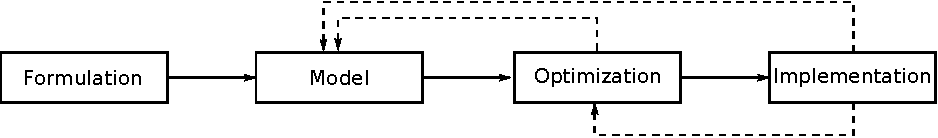
\includegraphics[width=0.75\textwidth]{01-introduction/img/decision_making_process}

\caption{A diagram of the classic decision-making process. Adapted from \cite{Talbi_Metaheuristics:2009}.\label{fig:01-decision_making_process}}
\end{figure}


\bigskip{}


Scientific computing, by means of computer-science methodology, enables
the study of problems that are too complex to be treated analytically,
or those that are very expensive or dangerous to be studied by direct
experimentation. Real-world problems are typically very complex systems
to be directly assessed by analytical models, and require a numerical
simulation for their study. Computer simulations provide a resource
to mimic the behavior of complex systems, by numerically evaluating
a model and gathering its data to estimate their true characteristics
\cite{law2007simulation}.

A model is a simplified representation of a studied problem, and one
of its purposes is to predict the effects of the variations within
the system. A good model is a balance between realism and simplicity.
The system simulation, on the other hand, is the operation of the
model. Its configuration can be changed, thus allowing multiple experimental
executions, something that might not be possible with the real system
it represents \cite{maria1997introduction}. However, it is important
to understand that the models used in scientific simulations and engineering
never offer a perfect representation of the system they resemble,
but only a subset of its composition and dynamics. For this reason,
experimentation and expert observation will always be essential as
reference points for understanding the studied phenomena. Consequently,
problems categorized as of large size and of considerable complexity
represent a challenge, because of the different involved disciplines
for their study and the degree of difficulty of their modeling. Cellular
radio networks in general, and those of the latest generations in
particular, fall under this categorization.


\section{Problem statement}

Radio networks represent one of the most fast-growing technology markets
since the introduction of the Global System for Mobile communications
(GSM\nomenclature[A]{GSM}{Global system for mobile communications})~\cite{3GPP_TR_50.099}.
As an implementation of the second generation of mobile networks (2G\nomenclature[A]{2G}{Second generation of mobile networks}),
GSM appeared more than twenty years ago. Its successor, the Universal
Mobile Telecommunications System (UMTS\nomenclature[A]{UMTS}{Universal mobile telecommunications system})~\cite{3GPP_TR_23.101}
marks an evolution from 2G, representing a milestone for the third
generation of mobile radio networks (3G\nomenclature[A]{3G}{Third generation of mobile networks}).
In recent years, the first commercial networks implementing the Long
Term Evolution (LTE\nomenclature[A]{LTE}{Long term evolution}), also
known as fourth generation (4G\nomenclature[A]{4G}{Fourth generation of mobile networks})
LTE, have also appeared~\cite{Gerstenberger-Introduction_to_LTE:2011}.
The always increasing demand for more bandwidth has been one of the
main forces behind the standardization and later implementation of
systems delivering higher-speed data services in order to improve
the user's experience.

This evolution, first from 2G to 3G and later from 3G to 4G, has introduced
not only the technology needed to increase data-transfer capacity
and voice quality, but also a greater complexity in terms of radio-network
planning, deployment, and configuration. This fact has attracted the
attention of the research community into areas such as the design
and optimization of radio-networks.

During the design phase of a radio network, a traditional or manual
approach comprises the software tool, i.e., the model in Figure~\ref{fig:01-decision_making_process},
that executes the analysis, and the human that makes the configuration
changes, i.e., the optimization in Figure~\ref{fig:01-decision_making_process}.
Therefore, a radio engineer manually adjusts the network parameters
and the software tool analyzes the given configuration. If the obtained
results are not acceptable, the analysis process has to be repeated
several times, until the goal is achieved and the changes are implemented,
i.e., the implementation in Figure~\ref{fig:01-decision_making_process}.
In the context of this thesis, this process is referred to as manual
radio-network optimization. 

Advances in the past few years have improved the manual optimization
process by introducing different problem-solving approaches that increase
the role of the computer during the optimization of radio networks,
consequently enlarging the scope of problems and instance sizes that
may be subject to optimization. Still, there are some important aspects
that restrict the automation level of these methods, not only in real-world
environments, but also when doing research in the area of radio networks:
\begin{itemize}
\item A selected optimization method is typically a compromise between solution
quality and computational-time complexity. The proposed state-of-the-art
approach for the evaluation of radio networks is the Monte-Carlo snapshot
analysis~\cite{Turke-Efficient_methods_for_WCDMA_radio_network_planning_and_optimization:2007,Wacker-Static_simulator_for_studying_WCDMA_radio_network_planning;1999}.
However, real-world environments, where radio-network design is carried
out, require the evaluation of networks with thousands of base stations
in a reasonable amount of time. Moreover, for applications involving
radio-network optimization, usually millions of evaluations are required
to find a good solution, in which case also snapshot simulations are
too time-consuming for practical use. Therefore, for such applications
and environments, methods with improved time efficiency are required.
\item A considerable number of publications in the field of radio-network
optimization, a few references of which are given for illustration
purposes~\cite{Amaldi-Radio_planning_and_coverage_optimization_of_3G_networks:2008,chen2008automated,Chen-Fast_algorithm_for_large_scale_UMTS_coverage_planning:2009,Antenna.azimuth.tilt:2009,Antenna.Configuration:2008,Siomina:Minimum.pilot.power.for.service.coverage},
base their simulations on platforms for which it is not possible to
reproduce the experiments, either because they have used proprietary
software or because the data is not available. This fact reduces the
possibilities for comparing different approaches among each other,
and significantly contrasts with other research areas, such as evolutionary
computing or numerical optimization, where several sets of open and
well-known benchmarks are available for the community to use. Consequently,
an open and unified framework should allow researchers to compare
different methods and results in a simplified and objective manner.
\item Available commercial tools for radio-network evaluation present several
drawbacks. In particular, regarding the size of networks that can
be considered and their computational-time complexity. Yet, even if
precise and fast methods were commercially available, they would lack
the level of flexibility required by the scientific community. Consequently,
an essential attribute of the framework is to be open source, so that
anyone can extend it to meet some specific requirements. In the long
term, this process should also extend the set of built-in functionality.
\item Particularly for path-loss predictions, estimated with empirical or
deterministic mathematical models, the inaccuracy of the input data
directly deteriorates the precision of the calculated results. Moreover,
since the physical properties that influence the propagation of radio
signals are not constant and every environment introduces its own
deviations, the calculated prediction may be considered as not more
than a rough approximation. Therefore, there is a need for a technique
that improves the accuracy of the state-of-the-art mathematical models
for radio propagations, despite the various sources of error noted
before.
\end{itemize}
This thesis introduces methods and tools to mitigate the above-mentioned
drawbacks from a radio-planning perspective.


\section{Hypotheses and approaches}

The work presented in this thesis is based on the following hypotheses
and their related approaches:
\begin{itemize}
\item Applying parallelization techniques should reduce the computational-time
requirement of the radio-propagation prediction, thus making it possible
to process larger, real-world radio networks.

\begin{itemize}
\item Unlike several examples in the literature of radio-network simulators,
which do not include support for parallel methods in order to reduce
the computational-time complexity, the unified framework includes
this feature in its basic structure. In this sense, parallel techniques
are used even when targeting a single computing host.
\end{itemize}
\item Using hardware, specialized for parallel execution (e.g., GPU), should
improve the execution time of parallel algorithms using threads or
message-passing mechanisms.

\begin{itemize}
\item From its arrival a few years ago, general GPU programming is continuously
gaining the attention of the research community and it is extending
to several areas of science. In particular, the combination of parallel-programming
techniques with GPU hardware should reduce the computational-time
requirement of the radio-propagation prediction even further.
\end{itemize}
\item Using the parallel framework for the objective-function evaluation
of different optimization problems should improve the quality of solutions
and enable tackling larger problem instances.

\begin{itemize}
\item On the one hand, a larger number of evaluations in the same amount
of time translates into a better exploration of the search space by
the optimization algorithm used. On the other hand, more complex or
exact models may be evaluated in the same amount of time, which implies
more accurate solutions.
\end{itemize}
\item Using the parallel framework to evaluate the objective function of
an automatic-optimization system should provide the means for solving
new, previously inaccessible optimization problems.

\begin{itemize}
\item The improved performance at the evaluation level opens new possibilities
for formally defining and tackling optimization problems that were
previously out-of-reach of state-of-the-art methods, either because
of their complexity or size.
\end{itemize}
\end{itemize}

\section{Scientific contributions}

The contributions of this thesis to the fields of telecommunications
and computer sciences include the following:
\begin{enumerate}
\item Design and development of a unified framework for radio-network planning
and optimization that supports computer clusters and GPUs.
\item Proposal of a new approach for parallel programming that enhances
the performance of a classic master-worker method.
\item Quality improvement of radio-propagation predictions by applying metaheuristic-optimization
techniques.
\item A new algorithm, based on autonomous agents, to tackle the service-coverage
problem in radio networks.
\item Identification and formalization of a new optimization problem in
radio networks.
\end{enumerate}

\section{Organization}

So far, a context has been provided for the following content of this
thesis. An introduction of the three research areas addressed by this
work, i.e., optimization, radio networks, and parallel methods, is
given in Chapters~\ref{chap:02-Optimization_models}, \ref{chap:02-Principles_of_mobile_radio_networks}
and~\ref{chap:02-Principles_of_GPU_programming}, respectively. They
provide an overview of the theoretical elements needed for a better
understanding of the rest of the thesis. Additionally, Chapter~\ref{chap:02-Optimization_of_radio_networks}
provides a short literature survey about the optimization of radio
networks. 

The unified framework for radio-network planning and optimization,
incorporating elements from the above-mentioned fields of study, is
presented in Chapter~\ref{chap:04-Framework-design-and-implementation}.

Chapters~\ref{chap:06-Experimental-evaluation-the-service-coverage-problem}
and~\ref{chap:07-Experimental-evaluation-the-SHO-alignment-problem}
demonstrate how the framework is applied to tackle two optimization
problems. In Chapter~\ref{chap:06-Experimental-evaluation-the-service-coverage-problem},
the problem of minimizing the total amount of pilot power subject
to a full coverage constraint is addressed with a novel approach.
Next, Chapter~\ref{chap:07-Experimental-evaluation-the-SHO-alignment-problem}
formally introduces a new optimization problem that deals with the
balancing of downlink and uplink soft-handover areas in UMTS networks.

The applicability and performance of the framework for radio-network
planning is validated in Chapters~\ref{chap:05-Framework_parameter_tuning}
and~\ref{chap:08-Real-world_network_planning}. Chapter~\ref{chap:05-Framework_parameter_tuning}
further extends the framework with automated-tuning capabilities that
enable its adaptation to different environments, thus improving the
accuracy of the radio-propagation predictions. In Chapter~\ref{chap:08-Real-world_network_planning},
the framework is tested in real network-planning conditions and compared
to a commercial, enterprise-level tool in terms of solution quality
and speed performance.

Finally, Chapter~\ref{chap:Conclusion} gives a short summary of
the thesis, outlines its main contributions and discusses further
work.


\section{Publications }

The work presented in this thesis is supported by a number of previous
publications. The initial work on the unified framework for radio-network
planning was published by Benedi\v{c}i\v{c} et al. in~\cite{Benedicic-A_GRASS_GIS_parallel_module_for_radio-propagation_predictions:2013}.
To address the challenges of the computational-time complexity during
optimization and its objective-function evaluations, Benedi\v{c}i\v{c}
et al. published the GPU extensions for the framework in~\cite{Benedicic-A_GPU_based_parallel_agent_optimization_approach:2013}.
The agent-based algorithm for solving the service-coverage problem
was initially published at the International multi-conference Information
Society~\cite{Benedicic_Pilot.power.optimization:2010}. This work
was further extended and later published in~\cite{Benedicic-A_GPU_based_parallel_agent_optimization_approach:2013}.
The primary ideas for the formal definition of the soft-handover balancing
problem were published at the World Congress of Computational Intelligence~\cite{Benedicic_Balancing_downlink_uplink_soft_handover_areas_in_UMTS_networks:2012}.
The results of the automated tuning capabilities of the framework
were published in~\cite{Benedicic-An_adaptable_parallel_simulation_framework_for_LTE_coverage_planning:2013}.

A comprehensive list of the author's publications is given in Appendix~A.


\cleardoublepage{}


\chapter{Background \label{chap:Background-and-motivation}}

% First paragraph has no indentation.

It is important to understand that the models used in scientific simulations
and engineering never offer a perfect model of the system they represent,
but only a subset of its composition and dynamics. Experimentation
and expert observation will always be essential as reference points
for understanding the studied phenomena.


\section{Radio-network optimization}

Once a mobile network is launched, an important part of its operation
and maintenance is monitoring the quality characteristics and changing
parameter values in order to improve its performance.

The evolution from 2G to 3G has introduced not only the technology
needed to increase both data and voice capacity, but also a greater
complexity in terms of network planning, deployment, and configuration,
which have rendered most of the traditionally used methods to be ineffective.
In a traditional approach (i.e. manual), during the network planning
and maintenance processes, a network planning software tool would
execute the analysis, while the human would make the change decisions.
Therefore, a radio planning engineer configures network parameters
manually and the network planning tool analyzes the given configuration.
If the obtained results are not acceptable, the analysis process has
to be repeated several times, until the goal is achieved.

Modern 3G radio networks are large and many of their key parameters
are interdependent. Since an engineer is not able to cope with the
level of complexity present in such systems, the computer, along with
specialized software, guides the engineer to the most appropriate
configuration for the network. In the context of this work, we will
refer to this process as optimization.

A common limitation of the implementations of such optimization methods,
generally targeting traditional computer architectures of sequential
execution, is their inability to meet the requirements needed by real-world
mobile networks, since their computational-time complexity make them
unfeasible for practical use. When analyzing big real-world networks
with thousands of users it is necessary to reduce the execution time
of the optimization processes as much as possible, so that they are
useful for practical use.

Additionally, the implementation of the framework will benefit from
valuable advances in computer science and High Performance Computing
(HPC), in order to perform faster and more reliable simulations \cite{gorder2007multicore,wen2011gpu}.

The complexity of these systems has grown even faster than their throughput
capacity, thus making it impossible to plan 3G mobile networks with
traditional methods. In this sense, an examination of colored coverage
maps in conjunction with some statistical analysis are no longer appropriate
tools for network examination. Once a mobile network is launched,
an important part of its operation and maintenance is monitoring of
quality characteristics and changing parameter values in order to
improve performance. In this sense, we may divide these tasks in two
phases: analysis and decision \cite{nawrocki2006understanding}. The
analysis phase consists of network performance analysis, which mainly
focuses on definition and collection of Key Performance Indicators
(KPIs). KPIs are quantifiable measurements, agreed to beforehand,
that reflect, in this context, network quality factors. The second
phase deals with making decisions, based on analytical results collected
in the previous phase, about the configuration of particular parameter
settings. This process (shown in Figure \ref{fig:Optimization-cycle})
is repeated until the achieved results are acceptable.

\begin{figure}
\centering

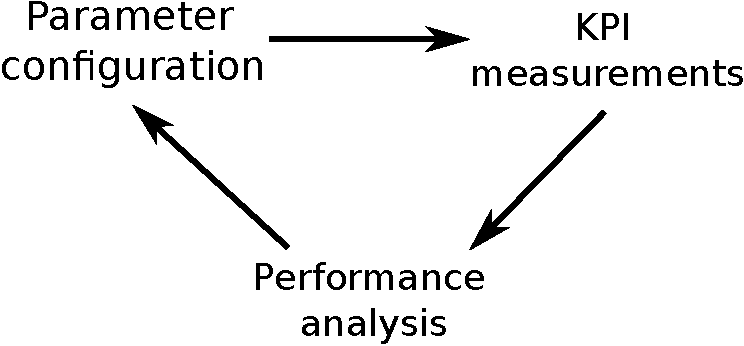
\includegraphics[width=0.4\textwidth]{02-background_and_motivation/img/optimization_cycle}

\caption{Optimization cycle for 3G mobile networks.\label{fig:Optimization-cycle}}
\end{figure}


In a traditional method approach (i.e. manual), during network planning
and optimization processes, a network planning software tool would
execute the analysis, while the human would make the decisions. Consequently,
a radio planning engineer configures network parameters manually and
the network planning tool analyzes the given configuration. If the
obtained results are not acceptable, the analysis process has to be
repeated several times, until the goal is achieved.

Modern 3G mobile networks are large and many of their key parameters
are interdependent. Since an engineer is not able to cope with the
level of complexity present in such systems, the computer, along with
specialized software, guides the engineer to the most appropriate
configuration for the network. In the context of this work, we will
refer to this process as \emph{optimization}. The results of the optimization
process are expected to provide advice%
\footnote{Some works are already focusing on complete automation of these tasks
(i.e. without human intervention).%
} regarding deployment, extension or reconfiguration tasks of a 3G
network.


\section{Optimization of 3G mobile networks}

Although wireless networks are increasingly more sophisticated, the
need for optimization work is still far from declining. It has been
established that most 3G radio network optimization problems are NP-hard,
since computational time grows non-polynomially with the increase
of the problem size \cite{amaldi:planning.umts.base.station.location}.
Moreover, there are other reasons directly related with the evolution
of already deployed networks that greatly increase the need for optimization
methods, as described in \cite{nawrocki2006understanding}:
\begin{itemize}
\item Network performance improvement: more users covered with the same
physical infrastructure, leaving room for parameter optimization only.
\item Changes in users\textquoteright{} profile: the introduction of new
services puts additional stress on the infrastructure, requiring additional
optimization efforts.
\item Changing propagation conditions: the allocation of a higher frequency
band for UMTS compared to GSM requires deployment of more 3G sites
than in 2G networks, mostly in urban areas, thus increasing inter-cell
interference.
\end{itemize}
In this sense, network operators have shown the need to define different
optimization targets. These targets are formed by an objective function
that maps possible values of configuration parameters into a value.
Thus, each element (solution) of the solution space is assigned a
comparable value, i.e. a real number. This number represents a quality
rating of the proposed solution and it is used to compare different
solutions among each other, and ultimately select the best one. Unfortunately,
there is no definitive objective function in the field of 3G network
optimization \cite{nawrocki2006understanding}. However, it is possible
to optimize for different targets such as coverage, base station location,
etc.

In this work, we will address network optimization methods that are
performed ``off-line'', meaning that the optimization software is
not an active functioning part of the network in operation. Statistical
data about network operation is used as the input or feedback information
for different optimization targets.

This paper gives an overview of well-known optimization problems in
3G mobile networks. At the beginning of each of the following sections,
a description of an optimization problem is given, followed by a short
survey of recently proposed optimization methods. Finally, a discussion
about the introduced methods is given, before closing with some concluding
remarks.


\section{Optimizing base station locations}


\subsection{Problem formulation}

Some references \cite{minimum.set.covering.problem:1997,minimum.set.covering.problem:1998,minimum.set.covering.problem:2000}
formulate the base station location problem in terms of the minimum
set covering problem (shown in Figure \ref{fig:The-minimum-set}).
The coverage problem is defined by considering the signal level in
every test point from all base stations and requiring that at least
one level is above a fixed threshold.

\begin{figure}[H]
\centering

\begin{minipage}[c]{0.45\textwidth}%
\centering

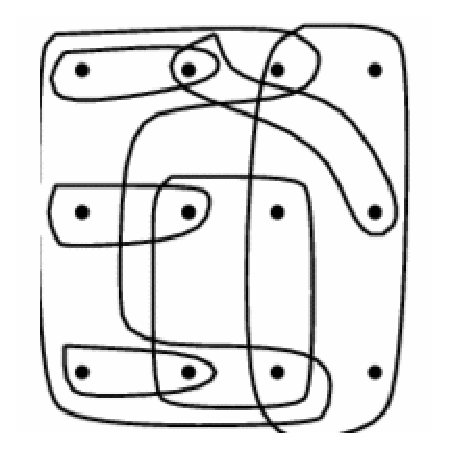
\includegraphics[width=0.6\textwidth]{02-background_and_motivation/img/set_cover_in}

(a)%
\end{minipage}\hfill{}%
\begin{minipage}[c]{0.45\textwidth}%
\centering

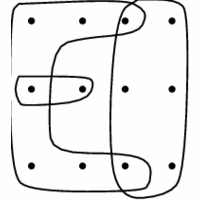
\includegraphics[width=0.6\textwidth]{02-background_and_motivation/img/set_cover_out}

(b)%
\end{minipage}\caption{The minimum set covering problem: (a) the problem input and (b) the
solution.\label{fig:The-minimum-set}}
\end{figure}


A different formulation considers the site selection problem as a
$p$-median problem, in which base station location is the only decision
variable considered. To each of the candidates solutions, an installation
cost is also associated. The $p$-median problem constitutes seeking
$p$ different locations each time, regardless of how distant the
sites are. The problem is to select one candidate site from each region
to install a base station such that the traffic capacity and the size
of the covered area are maximized with the lowest installation cost.


\subsection{Proposed solutions}

Aydin et al. \cite{Aydin:Heuristic.Optimization.Of.WCDMA} propose
a solution to the $p$-median problem based on three meta-heuristic
algorithms; a genetic algorithm, simulated annealing, and tabu search.
Their experimental study focuses on performance comparison between
the three algorithms.

A solution to the set covering problem is proposed by Hao et al. \cite{minimum.set.covering.problem:1997}.
A simulated annealing implementation was developed to solve the formulated
combinatorial problem. The results presented demonstrate the feasibility
of the proposed approach. Tutschku \cite{minimum.set.covering.problem:1998}
presents a specialized greedy algorithm to solve the same problem.
This work is part of the implementation of a planning tool prototype.
Mathar and Niessen \cite{minimum.set.covering.problem:2000} propose
a solution based on integer linear programming, which they claim finds
optimal solutions in most cases. They also introduce simulated annealing
as an approximate optimization technique. This approach substitutes
linear programming whenever an exact solution is out of reach because
of the complexity of the problem.

Amaldi et al. \cite{amaldi:planning.umts.base.station.location} offer
a discussion about the computational results of two different heuristics:
greedy search and tabu search. The problem formulation is based on
a set of candidate sites where the base stations can be installed,
an estimation of the traffic distribution and a propagation description
of the area to be covered. Some years later, the same authors \cite{Amaldi:Radio.planning.and.coveraga.optimization}
extended the problem formulation by also considering base station
configuration and hardware characteristics. In both works, they propose
a mixed integer programming model with which they aim to maximize
the trade-off between total traffic covered and total installation
costs. The only difference between the models is the constraint definition
of the linear program, where the constraints in \cite{amaldi:planning.umts.base.station.location}
are a subset of the constraints in \cite{Amaldi:Radio.planning.and.coveraga.optimization}.

Finally, Whitaker et al. \cite{GA.for.antenna.placement:2005} focus
on providing the required service coverage at the lowest possible
financial cost. Their framework supports the use of any multiple objective
optimization algorithm which seeks to approximate a Pareto front.
The performance of four different algorithms is explored, namely SEAMO,
SPEA2, NSGA-II and PESA.


\section{Optimizing antenna parameters}

There are many antenna parameters that control the coverage and interference
in the network, since the antenna shapes the emitted energy. Two important
parameters are the azimuth angle and the elevation angle (or tilt)
of the antenna. The antenna azimuth (shown in Figure \ref{fig:Antenna-azimuth})
is the direction in which the main beam of the horizontal pattern
points \cite{WCDMAforUMTS_RadioAccessForThirdGenerationMobileCommunications}.
The antenna tilt (shown in Figure \ref{fig:Antenna-tilt}) is defined
as the angle of the main beam of the antenna relative to the horizontal
plane \cite{WCDMAforUMTS_RadioAccessForThirdGenerationMobileCommunications}.
Both of these parameters have a great influence on network quality,
although antenna tilt requires less effort to implement, since most
modern radio networks already support remote electrical tilt. The
adjustment of these two parameters optimize some important aspects
of the network, namely:
\begin{itemize}
\item path loss between the base station and the mobile phone, since less
power is required for a connection, hence more power is available
for traffic; and
\item interference between neighboring cells, which leads to an overall
capacity increase.
\end{itemize}
\begin{figure}[h]
\centering

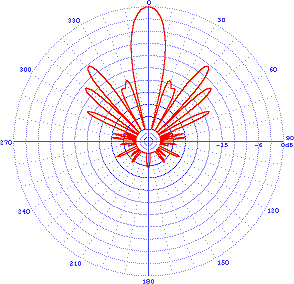
\includegraphics[width=0.3\textwidth]{02-background_and_motivation/img/azimuth}

\caption{A typical antenna azimuth pattern.\label{fig:Antenna-azimuth}}
\end{figure}


\begin{figure}
\centering

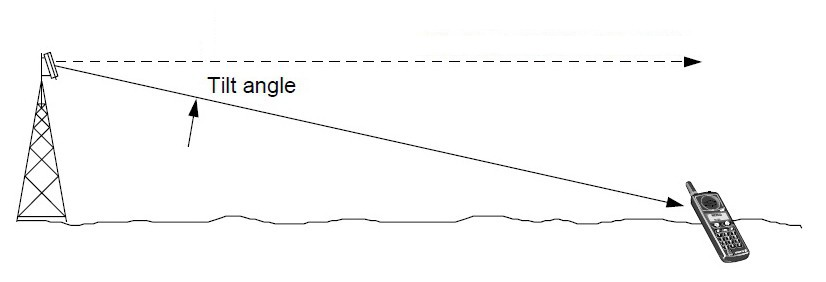
\includegraphics[width=0.6\textwidth]{02-background_and_motivation/img/tilt}

\caption{The antenna tilt angle with the horizontal plane.\label{fig:Antenna-tilt}}
\end{figure}



\subsection{Proposed solutions}

Karner \cite{MSc.antenna.optimization:2003} proposes an ``ad-hoc''
strategy for adjusting antenna azimuth and downtilt by analyzing the
structure of the network. The objective of this optimization is to
improve the results presented in \cite{Antenna.tilt.and.CPICH:2003}
by increasing the number of served users in the target area. In a
similar line of work, Jakl \cite{Jakl:PhD} included in his doctoral
thesis an antenna azimuth optimization algorithm, based on attempts
of avoiding coverage holes by properly adjusting the azimuth settings.

Siomina and Yuan \cite{Antenna.Configuration:2008} propose a framework
for automated optimization of antenna azimuth and tilt, including
both mechanical and electrical tilt. The implementation introduces
a simulated annealing algorithm that searches the solution space of
possible antenna configurations. The goal of the optimization is targeted
to address power sharing among cell channels and ultimately improve
High-Speed Downlink Packet Access (HSDPA) \cite{wiki:hsdpa} throughput.

Zhang et al. \cite{Antenna.azimuth.tilt:2009} present a method which
is composed of two optimization loops: the inner one and the outer
one. The inner loop concentrates on frequency planning while the outer
loop focuses on finding the optimal setting of antenna azimuth and
tilt for the current solution delivered by the inner loop. Although
frequency planning is not directly related to 3G network optimization,
we found this approach interesting enough to make a reference to it.
The inner loop could be easily replaced with some other optimization
target, e.g. common pilot channel power setting.


\section{Optimizing common pilot channel power}

The Common Pilot Channel (CPICH) is used as reference for handover
\cite{umts_world:handover}, cell selection \cite{3glteinfo:cellSelection},
and cell reselection \cite{flore2005:cell_reselection}. Whenever
a mobile phone is switched on, it tries to register with the cell
providing the highest received CPICH level. It also defines the effective
coverage area of the cell: according to the the CPICH power level,
the cell coverage area will enlarge or shrink. Consequently, by appropriately
adjusting the CPICH power at the base stations, the number of served
users per cell can be balanced among neighboring cells. This procedure
is called load balancing and it reduces interference, stabilizes network
operation, and facilitates radio resource management \cite{WCDMAforUMTS_RadioAccessForThirdGenerationMobileCommunications}.


\subsection{Proposed solutions}

Chen and Yuan \cite{CPICH.optimization:2008} optimize CPICH transmit
power starting from a uniform allocation (i.e. all cells are set with
the same transmit power level). Their objective is to enhance HSDPA
performance at cell edges while preserving control of R99 soft handover
\cite{wiki:soft_handover}. The solution approach is based on a linear-integer
mathematical model. A very similar problem and proposed solution is
presented by Siomina and Yuan \cite{CPICH.optimization:2007}. The
problem definition slightly differs from \cite{CPICH.optimization:2008}
as there is no reference to soft handover control. The solution is
also implemented as a linear program.

Olmos et al. \cite{CPICH.optimization:2003} apply simulated annealing
to the optimization of CPICH transmit powers in order to force mobile
phones to transmit to the best available cell in a service area. Their
results show decreased cell load with a consequently increased network
capacity.

Chen and Yuan \cite{CPICH.optimization:2009} present a two-phase
optimization algorithm for large-scale mobile networks. The algorithm
uses the total CPICH power consumption as a minimization objective.
The authors claim that the tabu-search-based algorithm can compute
near optimal solutions within a few seconds, even for large networks.


\section{Optimizing CPICH and antenna parameters}

Both the antenna tilt and azimuth directly affect the direction and
range in which the cell broadcasts its CPICH. Consequently, optimal
CPICH power is highly dependent on how the antenna tilt and azimuth
are configured at base stations. Ideal configuration of antenna tilt
and azimuth network-wise, with the objective of optimizing the CPICH
power consumption, is a challenging task. For this reason, many authors
have considered optimization methods that address all three parameters.


\subsection{Proposed solutions}

Varbrand et al. \cite{Coverage.optimization.on.CPICH.tilt.and.azimuth:2006}
approach the optimization of service coverage (see section \ref{sec:Optimizing-coverage})
by considering all three configuration parameters, namely: CPICH transmit
power, antenna tilt, and antenna azimuth. Their simulated annealing
algorithm searches the solution space of possible configurations in
order to find improvements in network performance and total transmitted
power. Interestingly, the algorithm is efficient enough to optimize
large networks without using excessive computing resources.

Siomina \cite{CPICH.and.antenna.tilt.optimization:2005} combines
optimization of base station antenna tilts and CPICH power to reduce
the total interference level and to improve network capacity. The
introduced algorithm optimizes the antenna downtilt setting so that
the total CPICH power in the network is minimized.

Neubauer et al. \cite{Antenna.tilt.and.CPICH:2003} present two optimization
algorithms for finding an optimal setting of antenna tilt and CPICH
power of the base stations. The first algorithm builds on a rule-based
approach, while the second one extends it by incorporating simulated
annealing. An evaluation of both techniques shows that the second
algorithm returns better results.

Jakl et al. \cite{GA.for.tilt.and.CPICH:2004} proposed a problem-specific
genetic algorithm to tackle the optimization of antenna tilts and
CPICH transmit powers. The goal of the optimization is to increase
network capacity. The implementation involves a deterministic fitness
selection scheme, a problem specific recombination operator and an
improved mutation operator. After the initial identification of the
best individuals, a local optimization technique is used to improve
their fitness.


\section{Optimizing coverage \label{sec:Optimizing-coverage}}

Coverage is maybe the most common optimization objective considered
in 3G network optimization. The objective function for coverage optimization
may be defined as follows:

\[
f_{cov}=\frac{A_{covered}}{A_{total}}
\]


where $A_{covered}$ represents the area covered by the network and
$A_{total}$ represents the total area under optimization. Thus, the
expression $f_{cov}$ represents the portion of the total area that
is actually under network coverage. This value ranges from 0 (no coverage)
to 1 (total coverage).

The area being optimized is usually divided in squares (or pixels)
of a certain size, which may vary from 10 to 100 meters, creating
a grid of a certain resolution. A square is considered covered, if
the signal to noise ratio is above a given threshold \cite{3GPP_TS_25.133}.
It is also common to use a test function $cov(x,y)$, which returns
1 if the square located at $(x,y)$ is covered, and 0 otherwise.


\subsection{Proposed solutions}

Siomina and Yuan \cite{Siomina:Minimum.pilot.power.for.service.coverage}
consider the problem of minimizing pilot power subject to the coverage
constraint. Their approach consists of mathematical programming models
and methods, based on a linear-integer mathematical formulation of
the problem. A special numerical analysis studies the trade-off between
service coverage and pilot power consumption for different test networks.

Capone et al. \cite{Amaldi:Radio.planning.and.coveraga.optimization}
investigate mathematical programming models for supporting decisions
on where to install new base stations and how to select their configuration
(antenna height and tilt, sector orientations, maximum emission power,
pilot signal, etc.) so to find a trade-off between maximizing coverage
and minimizing costs. The overall model takes into account signal-quality
constraints in both uplink and downlink directions, as well as the
power control mechanism and the CPICH signal.

Valkealahti et al. \cite{Coverage.balance:2002} propose a method
for automatic setting of CPICH power. The control algorithm applies
total transmission power measurements from the base station, neighboring
cells and mobile terminals to determine the pilot qualification. The
CPICH power is then periodically updated based on a group of heuristic
rules in order to improve coverage and load balance. A similar approach
is described by Parkinnen et al. \cite{Coverage.optimization.with.cost.function:2002}
where some network performance parameters are combined with service
coverage in a cost function. The pilot power of a cell is periodically
updated with a gradient descent method that minimizes the afore mentioned
function.


\section{Discussion}

In the field of 3G network optimization, comparing the efficiency
of different optimization methods has proven to be a very difficult
task. There are several reasons for this, among which we have identified
the following:
\begin{itemize}
\item The networks on which the experiments are carried out are not standardized.
Thus, it is problematic to set up an environment in which the presented
results may be reproduced.
\item There are no ``open'' implementations of 3G mobile network simulators.
On the contrary, there is a vast variety of proprietary (or ``closed'')
network simulators that only increase the ambiguity regarding the
experimental environment used for a certain network layout and configuration.
Moreover, some of the ``closed'' network simulators do not even
account on the built-in path loss estimation methods used.
\item Only a small part of the referenced optimization methods perform their
experiments on real-life networks, that have been already deployed
and are currently running. This fact creates a gap between the research
field and the industry (i.e. the application area) and it is counterproductive
for both the researchers and the network operators, since they don't
benefit from mutual collaboration.
\end{itemize}
We believe that the creation of a standardized framework would be
a great benefit in the field of 3G network optimization, as it would
allow researchers to compare different methods, results and solutions
in an easy, fast and objective manner. An effort in this direction
is the MOMENTUM project \cite{Momentum.project}. It was created with
the objective of setting up a standardized experimental environment
that would facilitate research cooperation and would ultimately benefit
from an improvement on the research field of 3G networks. The project
includes complete data about the terrain, properties of the service
area and hardware used in three different mobile networks. It offers
the researcher detailed information about real-life networks based
in Berlin, Lisbon and The Hague. As part of the package, there is
also a Java application programming interface (API) that eases the
implementation of some conventional tasks such as data parsing. The
main focus of project is on data, thus there is no network simulator
included. In any case, the researcher benefits from several included
traffic snapshots that help assessing different network configuration
settings. There have been no updates in the MOMENTUM project since
2005, when the last data corrections were introduced \cite{Momentum.project}.

In the context of this survey and after reviewing many different papers
on 3G network optimization, we can say that the MOMENTUM project has
not been widely adopted by the scientific community. Moreover, several
of the reviewed works do not offer detailed instructions on how to
resemble the experimental environment. Consequently, it is very complicated
(if not even impossible) to reproduce the presented results. Therefore,
the selection of optimization methods, based on the results presented
by their corresponding authors, is virtually meaningless, since the
results are not comparable with each other. For this reason, we have
decided to concentrate the following discussion on the optimization
methods used, leaving the results aside.


\subsection{The reproducibility problem}

A quick review of the state-of-the-art in 3G network optimization
indicates that software, providing good computational models, is a
very expensive tool for science. Moreover, since the vast majority
of this software is proprietary, it relies on closed source, formats
and protocols, which disclosure is explicitly forbidden by their licenses.
This fact creates a big hurdle to one of the key phases of scientific
methodology \cite{gauch2002scientific}: experimental reproducibility.


\subsection{Discussion about the presented methods}

Regarding the optimizations methods presented in previous chapters,
three distinctive groups emerge: genetic algorithms, linear programming
and other search methods.
\begin{description}
\item [{Genetic~algorithms}] These algorithms work on a population of
solutions that allows a more comprehensive search for optimal solutions.
As a direct consequence, an increase in running time is commonly observed.
The implementation effort of genetic algorithms is to some degree
higher than for simpler search methods (e.g. local search), but their
inherent structure greatly simplifies possible parallel implementations
and execution.
\item [{Linear~programming}] Linear optimization problems are widely used
in different optimization areas and there are many good software packages
to solve such problems. Consequently, if a problem can be modeled
as a continuous linear problem, there is usually no difficulty in
finding optimality. In the context of this survey, linear programming
has proven useful for coverage optimization in early network planning
stages.\\

\item [{Other~search~methods}] Other search methods%
\footnote{Namely, local search, simulated annealing and tabu search in the context
of this survey.%
} usually represent a compromise between running time and quality of
results. They rely on evaluating a great number of alternative configurations.
The number of parameters taken into account, as well as the evaluation
precision, directly influence their running time. These methods don't
excel in full simulation scenarios. On the other hand, some search
methods (e.g. tabu search) have powerful mechanisms to escape local
minima.
\end{description}
A short comparison of the optimization methods presented in this survey
is shown in Table \ref{tab:Comparison-of-optimization-methods}. The
comparison variables arise from the context in which the methods were
presented.

\begin{table}
\centering{\footnotesize \caption{A comparison among the presented optimization methods.\label{tab:Comparison-of-optimization-methods}}
}{\footnotesize \par}

{\footnotesize }%
\begin{tabular}{|c|c|c|}
\hline 
{\footnotesize Algorithm} & {\footnotesize Running time} & {\footnotesize Typical application}\tabularnewline
\hline 
\hline 
{\footnotesize Local search} & {\footnotesize Shorter} & {\footnotesize Solution quality improvement.}\tabularnewline
\hline 
{\footnotesize Tabu search} & {\footnotesize Shorter} & {\footnotesize Solution quality improvement.}\tabularnewline
\hline 
{\footnotesize Simulated annealing} & {\footnotesize Longer} & {\footnotesize Initial search of the solution space.}\tabularnewline
\hline 
{\footnotesize Genetic algorithm} & {\footnotesize Longer} & {\footnotesize Initial search of the solution space and solution quality
improvement.}\tabularnewline
\hline 
{\footnotesize Linear programming} & {\footnotesize (formulation dependent)} & {\footnotesize Coverage network planning.}\tabularnewline
\hline 
\end{tabular}
\end{table}



\section{Summary}

The variety of optimization problems that have been introduced in
the previous sections differ in many aspects like implementation,
running time and solution quality. Picking the right method for a
given situation depends on the optimization task and the desired results.
Since computation time is usually an important restriction, simpler
and faster methods may be preferable. 

Beside the convenience of a survey such as the one presented in this
work, it is very important to develop a feeling for the properties,
advantages and drawbacks of the respective methods. Moreover, radio
expert's recommendations regarding solution interpretation and feedback
from everyday network operation, are an essential input for creating
quality optimization methods. In this sense, and based on our own
experience, the expert's advice is irreplaceable and a most valuable
contribution to the research work.

Also, as it may be observed in some of the presented references, it
is often advisable to combine different methods. Therefore, a simple
optimization method may find a subset of reasonable parameter configuration,
whereas a more complex method could be applied afterward, to refine
the search. Sometimes it may also be useful to apply a simple search
method at the end to find better solutions in the vicinity of a current
promising one.


\cleardoublepage{}


\chapter{A Parallel Framework for Radio-Network Planning and Optimization
\label{chap:04-Framework-design-and-implementation}}

% First paragraph has no indentation.

In this chapter, a parallel framework for radio-coverage simulation
is presented. The objective of the framework is to provide an environment
for the radio-coverage prediction of large radio networks. Due to
its high performance, the framework also enables the evaluation of
more complex optimization problems for radio networks. 

The framework is implemented as a module of a geographical information
system, since the prediction calculation employs digital elevation
models and land-usage data. Following a master-worker parallel paradigm
over a message-passing communication model proved to be a bottleneck
for the performance of the parallel module. A new approach,that overcomes
this performance constraint is introduced in this chapter. The efficiency
improvement is based on overlapping process execution and communication.
This minimizes the idle time of the worker processes and thus improves
the overall efficiency of the system. To this end, the intermediate
calculation results are saved into an external database (DB\nomenclature[A]{DB}{Database system})
instead of sending them back to the master process. This approach
is implemented as part of a parallel radio-prediction tool (PRATO\nomenclature[A]{PRATO}{Parallel radio-prediction tool})
for the open-source Geographic Resources Analysis Support System (GRASS\nomenclature[A]{GRASS}{Geographic resources analysis support system})~\cite{Neteler_Open_source_GIS_a_GRASS_GIS_approach}.
An extended analysis of the experimental results is provided, which
are based on real data from an LTE network currently deployed in Slovenia.
Based on these experiments, which were performed on a computer cluster,
the new technique exhibits better scalability than the traditional
master-worker approach. Some real-world data sets are presented, the
coverage predictions of which are calculated in a shorter time while
saturating the hardware utilization.

The content of this chapter extends the research work published by
the author in~\cite{Benedicic-A_GRASS_GIS_parallel_module_for_radio-propagation_predictions:2013}.
The rest of this chapter is organized as follows. Section~\ref{sec:04-Motivation}
describes the motivation behind the presented research, followed by
an overview of the relevant publications in Section~\ref{sec:04-Related_work},
describing how they relate to this work. Section~\ref{sec:04-Radio_coverage_prediction_for_mobile_networks}
gives a description of the radio-coverage prediction problem, including
the radio-propagation model. Section~\ref{sec:04-Design_and_implementation}
concentrates on the design and implementation of the radio-propagation
tool, for both the serial and parallel versions. Section~\ref{sec:04-Simulations}
discusses the experimental results and their analysis.


\section{Motivation \label{sec:04-Motivation}}

Although Gordon Moore's well-known and often cited prediction still
holds \cite{Moore_Cramming_more_components_onto_integrated_circuits:1998},
the fact is that for the past few years, CPU speeds have hardly been
improving. Instead, the number of cores within a single CPU is increasing.
This situation poses a challenge for software development in general
and research in particular: a hardware upgrade will, most of the time,
fail to double the serial-execution speed of its predecessor. However,
since this commodity hardware is present in practically all modern
desktop computers, it creates an opportunity for the parallel exploitation
of these computing resources in order to enhance the performance of
complex algorithms over large data sets. The challenge is thus to
deliver the computing power of multi-core systems in order to tackle
a computationally time-consuming problem, the completion of which
is unfeasible using traditional serial approaches. Indeed, a performance
improvement opens new possibilities regarding the data sizes and accuracy
a model may handle.

A traditional approach, when dealing with computationally expensive
problem solving, is to simplify the models, thus reducing the time
needed for their calculation. Clearly, this method increases the introduced
error level, which is not an option for a certain group of simulations,
e.g., those dealing with disaster-contingency planning and decision
support~\cite{Huang_Using_adaptively_coupled_models_and_high_performance_computing_for_enabling_the_computability_of_dust_storm_forecasting:2012,Yin_A_framework_for_integrating_GIS_and_parallel_computing_for_spatial_control_problems_a_case_study_of_wildfire_dontrol:2012}.
The conducted simulations during the planning phase of a radio network
also belong to this group. The simulation results are the basis for
the decision making prior to physically installing the BSs and antennas
that will cover a certain geographical area. A larger deviation of
these results increases the probability of making the wrong decisions
at installation time, which may considerably increase the costs or
even cause mobile-network operators to incur losses.

Various researchers have successfully deployed HPC systems and techniques
to solve different problems dealing with spatial data~\cite{Akhter_Porting_GRASS_raster_module_to_distributed_computing:2007,Armstrong_Using_a_computational_grid_for_geographic_information_analysis:2005,Guan_A_parallel_computing_approach_to_fast_geostatistical_areal_interpolation:2011,Huang_Using_adaptively_coupled_models_and_high_performance_computing_for_enabling_the_computability_of_dust_storm_forecasting:2012,Li_Parallel_cellular_automata_for_large_scale_urban_simulation_using_load_balancing_techniques:2010,Osterman_CUDA_on_GRASS:2012,Tabik-High_performance_three_horizon_composition_algorithm_for_large_scale_terrains:2011,Tabik-Optimal_tilt_and_orientation_maps_a_multi_algorithm_approach_for_heterogeneous_multicore_GPU_systems:2013,Tabik_Simultaneous_computation_of_total_viewshed_on_large_high_resolution_grids:2012,Widener_Developing_a_parallel_computational_implementation_of_AMOEBA:2012,Yin_A_framework_for_integrating_GIS_and_parallel_computing_for_spatial_control_problems_a_case_study_of_wildfire_dontrol:2012}.
Their work confirms that a parallel paradigm such as master-worker,
and techniques like work pool (or task farming) and spatial-block
partitioning are applicable when dealing with parallel implementations
over large spatial data sets. However, it is well known that parallel
programming and HPC often call for area experts in order to integrate
them into a given environment~\cite{Clematis_High_performance_computing_with_geographical_data:2003}.
Moreover, the wide range of options currently available creates even
more barriers for general users wanting to benefit from HPC.

\bigskip{}


In this chapter, a high-performance, radio-planning framework for
GSM~(2G), UMTS~(3G) and LTE~(4G) networks is presented. Using a
snapshot-based approach (see Section~\ref{sec:06-Radio_network_model}),
the performance estimation of a radio network is divided into two
parts, i.e., the coverage prediction and the performance analysis.
During the coverage prediction, which is the subject of this chapter,
path-loss matrices are created based on radio-propagation models,
a network configuration, and digital maps of the target geographical
area. Hence, in addition to a reliable radio-propagation model, also
the resolution of the digital map should be high enough.

During the performance-analysis part, which is discussed in the following
chapters, the predicted path losses are used for analyzing different
phenomena, e.g., service availability and SHO performance. Therefore,
the largest influence on the result performance of the framework comes
from the calculated coverage predictions~\cite{Coinchon-The_impact_of_radio_propagation_predictions:2020}.

The framework is also suitable as a support tool for maintenance activities
related to network troubleshooting in general and optimization in
particular. Specifically, automatic radio-coverage optimization requires
the evaluation of millions of radio-propagation predictions in order
to find a good solution set. This is often unfeasible using other
serial implementations of academic or commercial tools~\cite{Ozimek_Open.source.radio.coverage.prediction:2010,Mehlfuhrer_The_Vienna_LTE_Simulators_enabling_reproducibility_in_wireless_communications_research:2011,Piro_Simulating_LTE_cellular_systems_an_open_source_framework:2011}.

As a reference implementation, the publicly available radio-coverage
prediction tool, presented in~\cite{Ozimek_Open.source.radio.coverage.prediction:2010},
was used. The authors developed a modular radio-coverage tool that
performs separate calculations for radio-signal path loss and antenna-radiation
patterns, also taking into account different configuration parameters,
such as antenna tilting, azimuth and height. The output result, saved
as a raster map, is the maximum signal level over the target area,
in which each point represents the received signal from the best-serving
transmitter (or cell). This work implements some well-known radio-propagation
models, e.g., Okumura-Hata~\cite{Hata_Empirical_formula_for_propagation_loss_in_land_mobile_radio_services:1980},
the description of which is later presented in Section~\ref{sub:04-Radio_propagation_model}.
Regarding the accuracy of the predicted values, the authors reported
comparable results to those of an industrial tool~\cite{Ozimek_Open.source.radio.coverage.prediction:2010}.
To ensure that the presented implementation is completely compliant
with this reference, a comparison test was designed that consists
of running both tools with the same set of input parameters. The test
results from PRATO and the reference implementation were identical
in all the tested cases.






\section{Related work \label{sec:04-Related_work}}

There are few examples of radio-network simulators in the literature~\cite{Ozimek_Open.source.radio.coverage.prediction:2010,Mehlfuhrer_The_Vienna_LTE_Simulators_enabling_reproducibility_in_wireless_communications_research:2011,Pillekeit-A_hybrid_simulation_framework_for_the_evaluation_of_common_RRM:2012,Piro_Simulating_LTE_cellular_systems_an_open_source_framework:2011,Sanchez_Performance_evaluation_of_OFDMA_wireless_systems_using_WM_SIM:2006,Yeung-Detailed_OFDM_modeling_in_network_simulation:2004}.
Most of these tools were developed for academic research, thus not
targeting industrial-sized environments. 

A Matlab-based LTE simulator was proposed in~\cite{Mehlfuhrer_The_Vienna_LTE_Simulators_enabling_reproducibility_in_wireless_communications_research:2011}.
It implements a standard LTE downlink physical layer, including Adaptive
Modulation and Coding (AMC\nomenclature[A]{AMC}{Adaptive modulation and coding}),
multiple users, Multiple Input Multiple Output (MIMO\nomenclature[A]{MIMO}{Multiple input multiple output})
transmission and scheduler. Despite being open source and freely available,
the fact of being implemented in Matlab makes it restrictive in terms
of tackling big problem instances of real networks.

A promising tool from the performance point of view was presented
in \cite{Piro_Simulating_LTE_cellular_systems_an_open_source_framework:2011},
where the authors implemented a full-stack LTE system in C++. Although
the tool has no graphical capabilities for displaying the simulation
progress or outcome, they might be included, since the source code
is available. In our opinion, the main drawback of this tool is the
lack of documentation, which makes it very difficult to continue extending
this work without the direct help of some of the original authors.

As an extension to the well-known NS-2 network simulator, Filiposka
and Trajanov \cite{Filiposka_Terrain_aware_three_dimensional_radio_propagation_model_extension_for_NS2:2011}
introduced a module for radio-propagation predictions, which takes
the terrain profile into account. In this case, the authors focus
on the relief, leaving out signal loss due to land-usage, which is
an important factor when targeting realistic radio-propagation scenarios.

\bigskip{}


The task-parallelization problem within the GRASS environment was
addressed by several authors in a variety of studies. For example,
in~\cite{Campos_Parallel_modelling_in_GIS:2012}, the authors presented
a collection of GRASS modules for a watershed analysis. Their work
concentrates on different ways of slicing raster maps to take advantage
of a Message Passing Interface (MPI\nomenclature[A]{MPI}{Message passing interface})
implementation.

In the field of HPC, the authors in~\cite{Akhter_Porting_GRASS_raster_module_to_distributed_computing:2007}
presented MPI and Ninf-G implementation examples of a GRASS raster
module that processes vegetation indexes from satellite images. The
authors acknowledge a limitation in the performance of their MPI implementation
for big processing jobs. The restriction appears due to the computing
nodes being fixed to a specific spatial range, since the input data
are equally distributed among worker processes, creating an obstacle
for load balancing in heterogeneous environments.

Using a master-worker technique, the work presented in~\cite{Huang-Explorations_of_the_implementation_of_a_parallel_IDW_algorithm_in_a_Linux_cluster:2011}
abstracts the GRASS data types into its own \emph{struct} and MPI
data types, thus not requiring the GRASS in the worker nodes. The
data are evenly distributed by rows among the workers, with each one
receiving an exclusive column extent to work on. Their test cluster
contained heterogeneous hardware configurations. The authors noted
that data-set size is bounded by the amount of memory on each of the
nodes, since they allocate the memory for the whole map as part of
the set-up stage, before starting the calculation. Regarding the data
sets during the simulations, the largest one contained 3,265,110 points.
They concluded that the data-set size should be large enough for the
communication overhead to be hidden by the calculation time, so that
the parallelization pays off.

In~\cite{Tabik-High_performance_three_horizon_composition_algorithm_for_large_scale_terrains:2011},
the authors employed a master-worker approach, using one worker process
per worker node. The complete exploitation of the computing resources
of a single computing node is achieved with OpenMP. The experimental
environment featured one host. The horizon-composition algorithm presents
no calculation dependency among the spatial blocks. Consequently,
the digital elevation model (DEM\nomenclature[A]{DEM}{Digital elevation model})
was divided into separate blocks to be independently calculated by
each worker process. The authors presented an improved algorithm that
can also be used to accelerate other applications like visibility
maps. The tasks are dynamically assigned to idle processes using a
task-farming paradigm over the MPI. 

Similar to~\cite{Tabik-High_performance_three_horizon_composition_algorithm_for_large_scale_terrains:2011},
in~\cite{Tabik-Optimal_tilt_and_orientation_maps_a_multi_algorithm_approach_for_heterogeneous_multicore_GPU_systems:2013}
there was no calculation dependency among the spatial blocks. The
experimental evaluation was made over multiple cores of one CPU and
a GPU, and a master-worker setup was used for process communication.

In~\cite{Yin_A_framework_for_integrating_GIS_and_parallel_computing_for_spatial_control_problems_a_case_study_of_wildfire_dontrol:2012},
the authors presented a parallel framework for GIS integration. Based
on the principle of spatial dependency, they lowered the calculation-processing
time using a knowledge database, delivering the heavy calculation
load to the parallel back-end if a specific problem instance is not
found in the database. There was an additional effort to achieve the
presented goals, since the implementation of a fully functional GIS
(or ``thick GIS'' as the authors call it) was required on both the
desktop client and in the parallel environment.

An agent-based approach for simulating spatial interactions was presented
in~\cite{Gong_Parallel_agent_based_simulation_of_individual_level_spatial_interactions_within_a_multicore_computing_environment:2012}.
This technique decomposes the entire landscape into equally-sized
regions, i.e., a spatial-block division as in \cite{Tabik-High_performance_three_horizon_composition_algorithm_for_large_scale_terrains:2011},
which are in turn processed by a different core of a multi-core CPU.
This work used multi-core CPUs instead of a computing cluster.

Some years ago, grid computing received a lot of attention from the
research community. It appeared to be a good alternative for accessing
the extra computational power needed for the spatial analysis of large
data sets~\cite{Armstrong_Using_a_computational_grid_for_geographic_information_analysis:2005,Vouk_Cloud_computing_issues_research_and_implementations:2008,Wang_A_cybergis_framework_for_the_synthesis_of_cyberinfrastructure_GIS_and_spatial_analysis:2010}.
However, several obstacles are still preventing this technology from
being widely used. In particular, its adoption requires not only hardware
and software compromises with respect to the involved parts, but also
a behavioral change at the human level~\cite{Armstrong_Using_a_computational_grid_for_geographic_information_analysis:2005}.


\section{Radio-coverage prediction for mobile networks \label{sec:04-Radio_coverage_prediction_for_mobile_networks}}


\subsection{Background}

As it was mentioned in Chapter~\ref{chap:02-Principles_of_mobile_radio_networks},
radio communications in a mobile network take place between a BS (or
fixed transmitter) and a number of UEs (or mobile receivers). The
effects of signal propagation limit the performance of a mobile-radio
system. For this reason, the characterization and modeling of radio
propagation is considered a fundamental aspect in radio-network planning
\cite{Ahmad:Studying_different_propagation_models_for_LTE_system:2012}.
Consequently, understanding the mathematical modeling of a frequency
channel is necessary to accurately predict the system performance
and to provide a mechanism to analyze the effects caused by signal
propagation \cite{Parsons-The_mobile_radio_propagation_channel:2000}.

The coverage planning of radio networks is a key problem that all
mobile operators have to deal with. Moreover, it has proven to be
a fundamental issue, not only in LTE networks, but also in other standards
for mobile communications~\cite{Saleh_On_the_coveraga_extension_in_LTE_networks:2010,Shabbir_Comparison_of_radio_propagation_models:2011,Siomina:Minimum.pilot.power.for.service.coverage,Valcarce_Applying.FDTD.to.the.coverage.prediction.of.WiMAX:2009}.
One of the primary objectives of mobile-network planning is to efficiently
use the allocated frequency band to ensure that some geographical
area of interest can be satisfactorily reached with the BSs of the
network. To this end, radio-coverage prediction tools are of great
importance, as they allow network engineers to test different network
configurations before physically implementing the changes. Radio-coverage
prediction is a complex task, mainly due to the several combinations
of hardware and configuration parameters that have to be analyzed
in the context of different environments. The complexity of the problem
means that radio-coverage predictions are computationally-intensive
and time-consuming, hence the importance of using fast and accurate
tools (see Section~\ref{sub:04-Computational_complexity} for a complexity
analysis of the algorithm). Additionally, since the number of deployed
transmitters keeps growing with the adoption of modern standards~\cite{Saleh_On_the_coveraga_extension_in_LTE_networks:2010},
there is a clear need for a radio-propagation tool that is able to
cope with larger work loads in a feasible amount of time (see Section~\ref{sub:04-Computational_complexity}
for the running time of the serial version).


\subsection{Radio-propagation model \label{sub:04-Radio_propagation_model}}

PRATO uses a modified version of the well-known Okumura-Hata model
for radio-propagation predictions~\cite{Hata_Empirical_formula_for_propagation_loss_in_land_mobile_radio_services:1980}.
Other accurate methods exist, like the ones based on ray tracing~\cite{Corre_Three_dimensional_urban_EM_wave_propagation_model_for_radio_network_planning_and_optimization_over_large_areas:2009,Vilhar-Efficient_open_source_ray_tracing_methods_for_rural_environment:efficient}.
However, these methods are more sensible to deviations in input data,
like DEMs and buildings, and are still inefficient in terms of the
computational effort required to achieve satisfying results. Empirical
methods for radio-propagation predictions, like Okumura-Hata, give
acceptable results within a feasible amount of time. For this reason,
they have become the industry standard for non-deterministic signal-propagation
calculations~\cite{Begovic_Applicability_evaluation_of_Okumura_Ericsson_and_Winner_propagation_models_for_coverage_planning:2012,Cichon_Propagation.prediction.models:1995,Hata_Empirical_formula_for_propagation_loss_in_land_mobile_radio_services:1980,Shabbir_Comparison_of_radio_propagation_models:2011,Song_Evolved_cellular_network_planning_and_optimization_for_UMTS_and_LTE:2010}.

The Okumura-Hata model has been largely studied and shown to be suitable
for predicting the radio propagation in LTE networks~\cite{Ahmad:Studying_different_propagation_models_for_LTE_system:2012,Shabbir_Comparison_of_radio_propagation_models:2011}.
In its primary form, the model distinguishes the distance from the
receiver to the transmitter, the frequency used and the effective
antenna height, i.e., the height of the antenna above the receiver's
level. These variables are taken into account in order to calculate
the path loss in open-area (OA\nomenclature[A]{OA}{Open area}) conditions.
Additionally, for distinguishing non-line-of-sight (NLOS\nomenclature[A]{NLOS}{Non line of sight})
conditions, the terrain profile and Earth shape are added to the original
formula. In this context, a NLOS situation appears when the first
Fresnel zone is obscured by at least one obstacle. A Fresnel zone
is defined as one of the concentric ellipsoids which define volumes
in the radiation pattern of a circular aperture~\cite{Xia-Radio_propagation_characteristics_for_line_of_sight_microcellular_and_personal_communications:1993}.

As it was mentioned before, the path-loss evaluation employed here
is based on the Okumura-Hata model. When in an OA environment, the
path loss is described as in Equation~(\ref{eq:04-Hata_OA}):

\begin{eqnarray}
\mathrm{L}{}_{\mathrm{OA}}(d_{(x,y)},\vec{\beta}) & = & \beta_{0}+\beta_{1}\log(d_{(x,y)})+\beta_{2}\log(H_{\mathrm{A}})+\beta_{3}\log(d_{(x,y)})\log(H_{\mathrm{A}})-\nonumber \\
 &  & 3.2\left[\log(11.75\cdot H_{\mathrm{R}})\right]^{2}+44.49\log(F)-4.78\left[\log(F)\right]^{2},\label{eq:04-Hata_OA}
\end{eqnarray}


\noindent \nomenclature[S]{$\mathrm{L}_{\mathrm{OA}}$}{Path loss in an open-area environment}\nomenclature[S]{$\vec{\beta}$}{Control-parameter vector of the path-loss model}\nomenclature[S]{$d_{(x,y)}$}{Distance from the cell to the topography point with coordinates $(x,y)$}\nomenclature[S]{$H_A$}{Antenna height above the receiver}\nomenclature[S]{$H_R$}{Height of the receiver antenna above ground level}

\noindent where $\vec{\beta}=(\beta_{0},\beta_{1},\beta_{2},\beta_{3})$
is the vector containing the control parameters of the model, $d_{(x,y)}$
is the distance (in kilometers) from the transmitter to the topography
point with coordinates $(x,y)$, $H_{\mathrm{A}}$ is the effective
antenna height (in meters) of the transmitter, $H_{\mathrm{R}}$ is
the antenna height (in meters) of the receiver, and $F$ is the frequency,
expressed in MHz. In NLOS conditions, the additional path loss is
calculated as in Equation~(\ref{eq:04-Hata_NLOS}):

\begin{equation}
\mathrm{L}{}_{\mathrm{NLOS}}(d_{(x,y)})=\sqrt{\left[\alpha K(d_{(x,y)})\right]^{2}+E(d_{(x,y)})^{2}},\label{eq:04-Hata_NLOS}
\end{equation}


\noindent \nomenclature[S]{$\mathrm{L}_{\mathrm{NLOS}}$}{Path loss in non-line-of-sight conditions}\nomenclature[S]{$\alpha$}{Knife-edge diffraction control parameter}\nomenclature[S]{$K(d_{(x,y)})$}{Knife-edge diffraction loss}\nomenclature[S]{$E(d_{(x,y)})$}{Loss correction due to the Earth sphere}

\noindent where $\alpha$ is the knife-edge diffraction%
\footnote{\noindent Knife-edge diffraction occurs when a portion of the incident
radiation reaches a well-defined obstacle, such as a mountain or the
edge of a building.%
} control parameter, the value of which is calculated based on the
level of obstruction of a Fresnel zone, $K(d_{(x,y)})$ is the knife-edge
diffraction loss (in~dB), and $E(d_{(x,y)})$ is the correction due
to the Earth sphere (in~dB). All three values depend on the characteristics
of the topography point with coordinates $(x,y)$.

In this work, as well as in~\cite{Filiposka_Terrain_aware_three_dimensional_radio_propagation_model_extension_for_NS2:2011},
the terrain profile is used for line-of-sight (LOS\nomenclature[A]{LOS}{Line of sight})
determination, i.e., an obstacle obstruction in the first Fresnel
zone of the transmitter. In order to adequately predict signal-loss
effects due to foliage, buildings and other fabricated structures,
additional loss factors based on the land usage (clutter data), are
included. This technique is adopted by several propagation models
for radio networks~\cite{Aarnaes-Tuning_of_empirical_radio_propagation_models_effect_of_location_accuracy:2004,Begovic_Applicability_evaluation_of_Okumura_Ericsson_and_Winner_propagation_models_for_coverage_planning:2012,Neskovic_Microcell_electric_field_strength_prediction_model:2010}.
Consequently, an extra term is introduced for signal loss due to clutter,
thus defining the model-predicted path loss as:

\begin{equation}
\mathrm{L}(d_{(x,y)},\vec{\beta})=\mathrm{L}{}_{\mathrm{OA}}(d_{(x,y)},\vec{\beta})+\mathrm{L}_{\mathrm{NLOS}}(d_{(x,y)})+\mathrm{L}{}_{\mathrm{CLUT}}(d_{(x,y)}),\label{eq:04-Hata_pathloss}
\end{equation}


\noindent \nomenclature[S]{$\mathrm{L}(d_{(x,y)})$}{Path loss at the topography point with coordinates $(x,y)$}\nomenclature[S]{$\mathrm{L}_{\mathrm{CLUT}}$}{Signal loss due to clutter}

\noindent where $\mathrm{L}{}_{\mathrm{CLUT}}(d_{(x,y)})$ represents
a look-up function for the clutter loss at the topography point with
coordinates $(x,y)$, expressed in dB, which are given as input data.


\section{Design and implementation \label{sec:04-Design_and_implementation}}


\subsection{Geographic resources analysis support system}

GRASS~\cite{Neteler_Open_source_GIS_a_GRASS_GIS_approach}, a free
and open-source software project that implements a Geographical Information
System (GIS\nomenclature[A]{GIS}{Geographical information system}),
is used as the software environment for PRATO. This GIS software was
originally developed at the US Army Construction Engineering Research
Laboratories and is a full-featured system with a wide range of analytical,
data-management, and visualization capabilities. Currently, the development
of GRASS GIS is supported by a growing community of volunteer developers.

The use of GRASS GIS as an environment for PRATO presents many advantages.
First, the current development of GRASS is primarily Linux-based.
Since the field of HPC is dominated by Linux and UNIX systems, an
environment with Linux support is critical for this work. Software
licensing is another important consideration for choosing GRASS, since
it is licensed under the GNU Public License \cite{Stallman_GNU_License:1991}
that imposes the availability of the source code. This allows to make
potential modifications to the system, thus adapting it for the parallel
computation environment. Moreover, GRASS provides a great deal of
built-in functionality, capable of operating with raster and vector
topological data that can be stored in an internal format or a DB.


\subsection{Multi-paradigm parallel programming}

The implementation methodology adopted for PRATO follows a multi-paradigm,
parallel programming approach in order to fully exploit the resources
of each node in a computing cluster. This approach combines a master-worker
paradigm with an external DB. To efficiently use a shared memory multi-processor
on the worker side, and to effectively overlap the calculation and
communication, PRATO uses POSIX threads~\cite{Butenhof_Programming.with.POSIX.threads:1997}.

To use the computing resources of a distributed memory system, such
as a cluster of processors, PRATO uses the MPI~\cite{Gropp_Using_MPI:1999}.
The MPI is a message-passing standard that defines the syntax and
semantics designed to function on a wide variety of hardware. The
MPI enables multiple processes, running on different processors of
a computer cluster, to communicate with each other. It was designed
for high performance on both massively parallel machines and on workstation
clusters.

PRATO also supports the execution of the most computationally-intensive
parts of the radio-propagation algorithm on a GPU. Moreover, the GPU
hardware is used if it is available on the computing nodes that host
the worker processes (see Section~\ref{sub:04-GPU_worker_implementation}
later in this chapter for a discussion about the GPU implementation).

In order to make the text clearer and to differentiate between the
programming paradigms used from here on, a POSIX thread will be referred
to simply as a 'thread' and a MPI process as a 'process'.


\subsection{Design of the serial version}

This section describes the different functions contained in the serial
version of PRATO, which is implemented as a GRASS module. Their connections
and data flow are depicted in Figure~\ref{fig:04-Flow_diagram_serial_version},
where the parallelograms of the flow diagram represent the input/output
(I/O\nomenclature[A]{I/O}{Input/output}) operations. 

The design follows a similar internal organization as the radio-planning
tool presented in \cite{Ozimek_Open.source.radio.coverage.prediction:2010},
but with some important differences. Specifically, the design presented
here employs a direct connection to an external database server for
intermediate result saving, instead of the slow, built-in GRASS database
drivers. To explicitly avoid tight coupling with a specific database
vendor, the generated output is formatted in plain text, which is
then forwarded to the DB. Any further processing is achieved by issuing
a query over the database tables that contain the path-loss results
for each of the processed transmitters.


\subsubsection{Input parameters}

All input data are read in the first step (see ``Read input data''
in Figure~\ref{fig:04-Flow_diagram_serial_version}). Their formats
differ based on the data they contain, i.e.:
\begin{itemize}
\item GRASS raster files are used for the DEM and clutter data, whereas
\item a text file is used for the transmitter configurations and other service-dependent
options.
\end{itemize}
Since the module accepts a considerable amount of input parameters,
they are read from a text-based initialization (INI\nomenclature[A]{INI}{Initialization file})
file. This is far more practical than passing them as command-line
parameters, which would make them error-prune and difficult to read.
Besides, the INI file may contain configuration parameters for many
transmitters. The user selects which one(s) to process at run-time
by passing a command-line option.

\begin{figure}
\centering

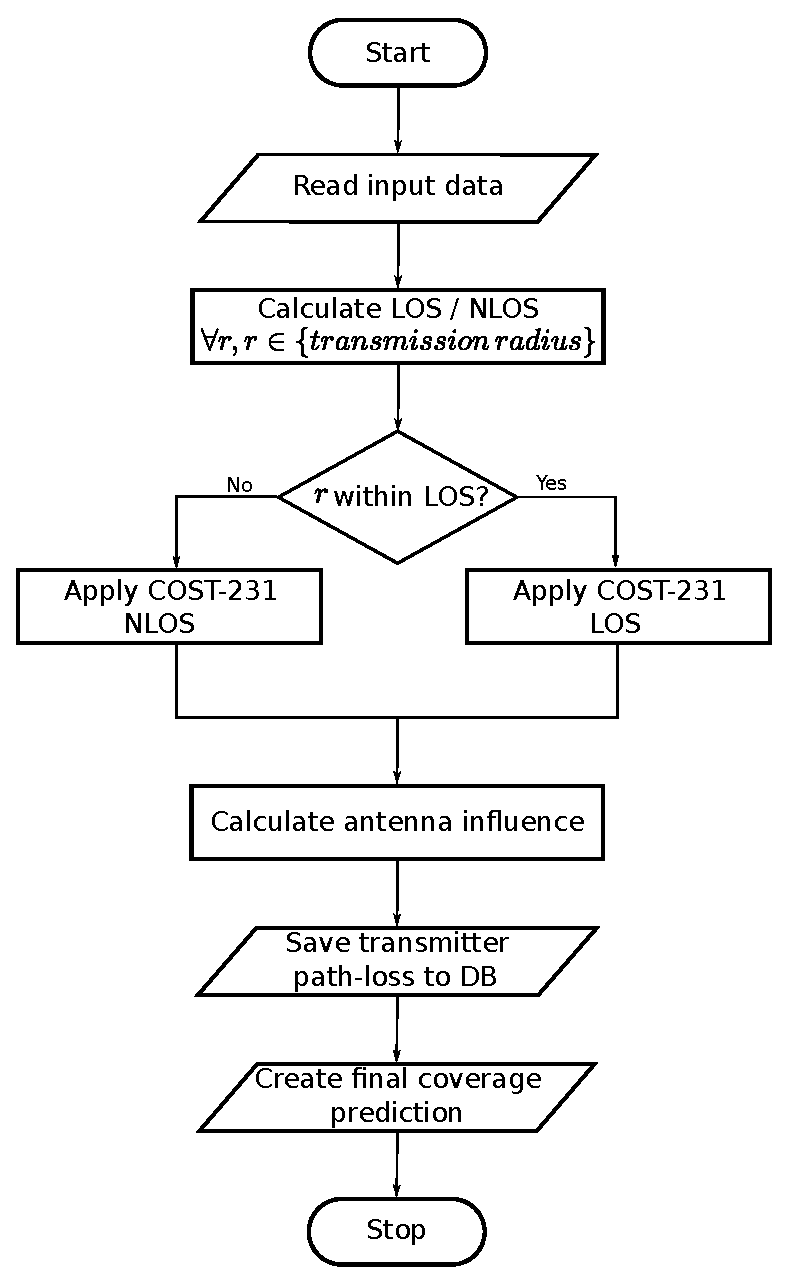
\includegraphics[width=1\columnwidth]{04-framework_design_and_implementation/img/serial_implementation_flow_diagram}

\caption{\textit{\emph{Flow diagram of the serial version.}}\textit{\label{fig:04-Flow_diagram_serial_version}}}
\end{figure}



\subsubsection{Isotropic path-loss calculation\label{sub:04-Isotrophic_pahloss_calculation}}

This step starts by calculating which receiver points, $r$, are within
the specified transmission radius (see ``\emph{transmission radius}''
in Figure~\ref{fig:04-Flow_diagram_serial_version}). The transmission
radius is defined around each transmitter in order to limit the radio-propagation
calculation to a reasonable distance. For these points, the path loss
for an isotropic source (or omni antenna) is calculated. This calculation
is performed by applying the radio-propagation model, which was previously
defined in Equation~(\ref{eq:04-Hata_pathloss}), to each of the
points within the transmission radius around the transmitter (see
``Calculate path loss'' in Figure~\ref{fig:04-Flow_diagram_serial_version}).

Figure~\ref{fig:04-Raster_path_loss_example} shows an example of
the isotropic path-loss calculation, only including the map area within
the transmission radius. The color scale is given in dB, indicating
the signal loss from the isotropic source of the transmitter, located
at the center. Notice the hilly terrain is clearly distinguished due
to LOS and NLOS conditions from the signal source.

\begin{figure}
\centering

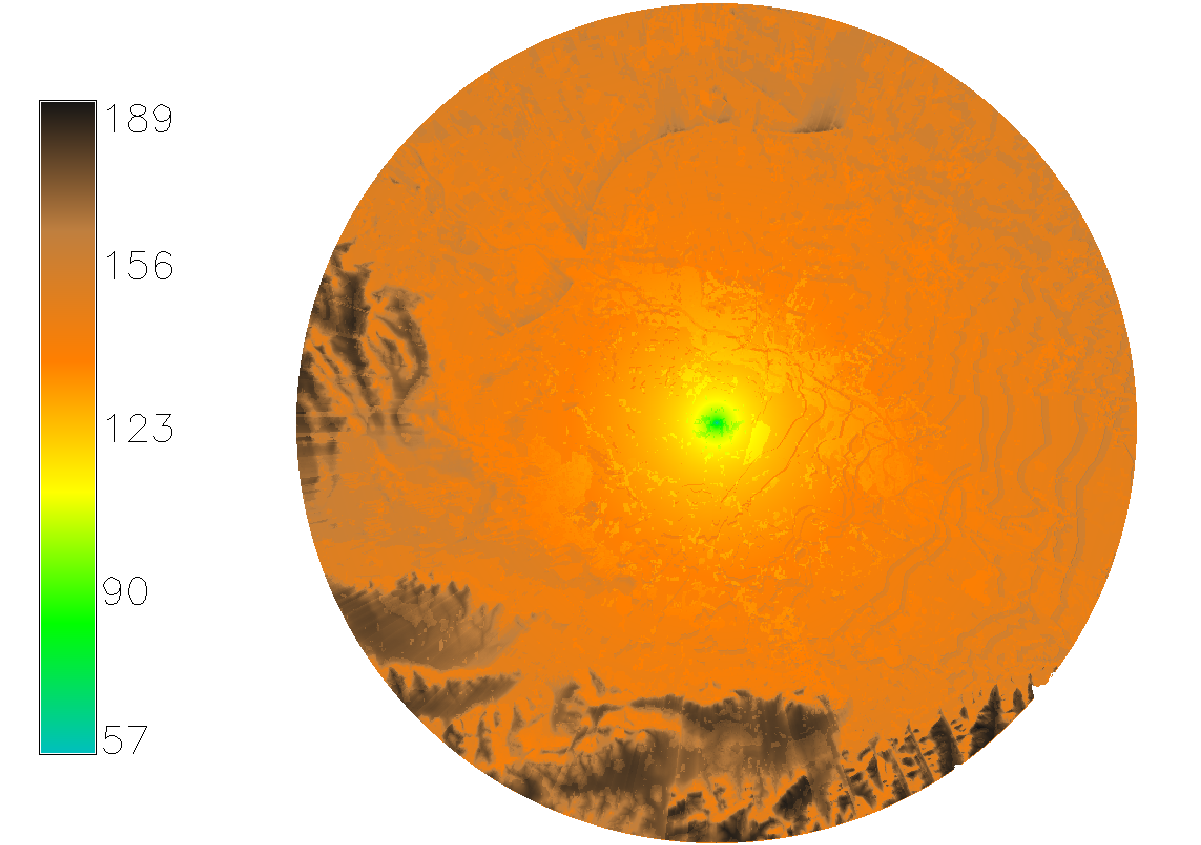
\includegraphics[width=0.6\textwidth]{04-framework_design_and_implementation/img/isotrophic_calculation}

\caption{\textit{\emph{Example of a raster map, showing the result of a path-loss
calculation from an isotropic antenna. The color scale is given in
dB, indicating the path loss at a given point. \label{fig:04-Raster_path_loss_example}}}}
\end{figure}



\subsubsection{Antenna diagram influence \label{sub:04-Antenna_diagram_influence}}

This step considers the antenna radiation diagram of the current transmitter
and its influence over the isotropic path-loss calculation (see ``Calculate
antenna influence'' in Figure~\ref{fig:04-Flow_diagram_serial_version}).
Working on the in-memory results generated by the previous step, the
radiation diagram of the antenna is taken into account, including
the beam direction, the electrical and the mechanical tilt. Figure~\ref{fig:04-Raster_antenna_example}
shows the map area within the transmission radius, where this calculation
step was applied to the results from Figure~\ref{fig:04-Raster_path_loss_example}.
Notice the distortion of the signal propagation that the antenna has
introduced.

\begin{figure}[h]
\centering

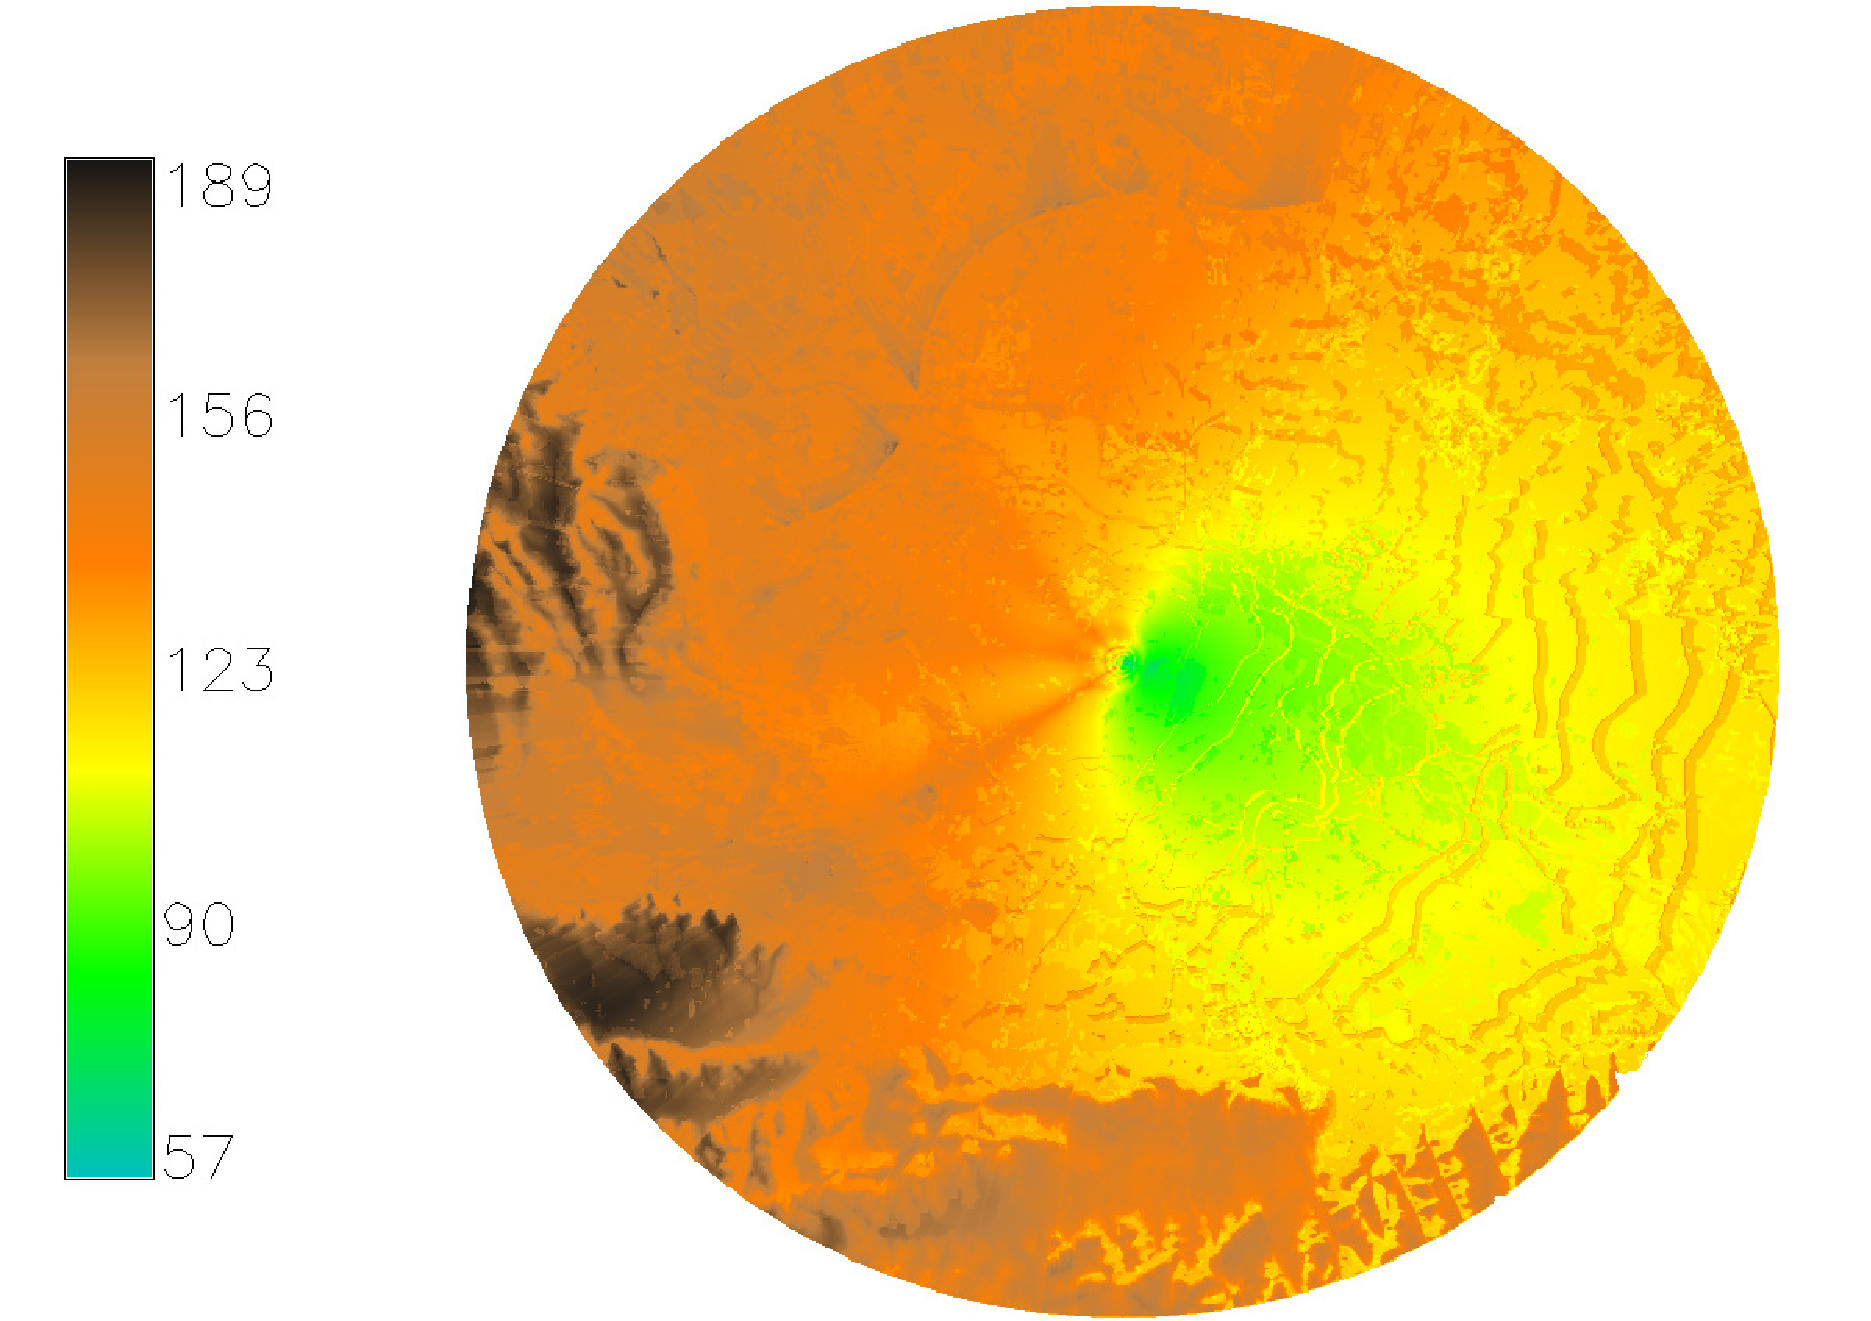
\includegraphics[width=0.6\textwidth]{04-framework_design_and_implementation/img/antenna_calculation}

\caption{\textit{\emph{Example of a raster map, showing the influence of a
directional antenna over the path-loss result depicted in Figure~\ref{fig:04-Raster_path_loss_example}.
The color scale is given in dB, indicating the path loss at a given
point. \label{fig:04-Raster_antenna_example}}}}
\end{figure}



\subsubsection{Transmitter path-loss prediction \label{sub:04-Transmitter_path_loss_prediction}}

In this step, the path-loss prediction of the transmitter is saved
in its own database table (see ``Save transmitter path-loss to DB''
in Figure~\ref{fig:04-Flow_diagram_serial_version}). This is accomplished
by connecting the standard output of the GRASS module with the standard
input of a database client. Naturally, the generated plain text should
be understood by the DB itself.


\subsubsection{Coverage prediction \label{sub:04-Coverage_prediction}}

\begin{figure}
\centering

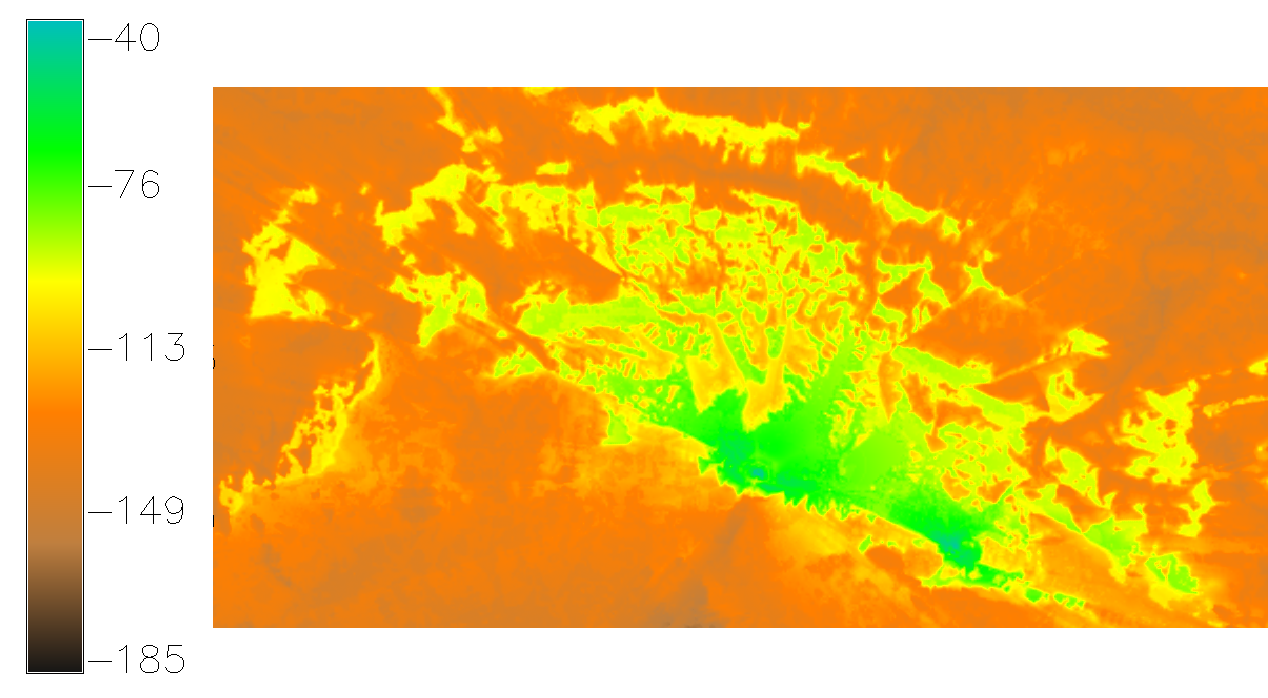
\includegraphics[width=0.65\textwidth]{04-framework_design_and_implementation/img/final_coverage}

\caption{\textit{\emph{Example of a raster map, displaying the final coverage
prediction of 136 transmitters over a geographical area. The color
scale is given in dBm, indicating the received-signal strength. Darker
colors denote areas with a reduced signal due to the fading effect
of the hilly terrain and clutter. \label{fig:04-Raster_prediction_example}}}}
\end{figure}


The final radio-coverage prediction, containing the aggregation of
the partial path-loss results of the involved transmitters, is created
in this step (see ``Create final coverage prediction'' in Figure~\ref{fig:04-Flow_diagram_serial_version}).
The received signal strength from each of the transmitters is calculated
as the difference between its transmit power and the path loss for
the receiver's corresponding position. This is done by executing an
SQL query over the tables containing the path-loss predictions of
each of the processed transmitters. Finally, the output is generated
using the GRASS built-in modules $v.in.ascii$ and $v.to.rast$, which
create a raster map using the query results as the input. The resulting
raster map contains the maximum received signal strength for each
individual point, as shown in Figure~\ref{fig:04-Raster_prediction_example}.
In this case, the color scale is given in dBm, indicating the strongest
received signal strength from the transmitters.


\subsection{Computational complexity \label{sub:04-Computational_complexity}}

\begin{algorithm}
\centering

\caption{Pseudo-code of the radio-coverage prediction algorithm. The time complexity
is given per line.\label{alg:04-Pseudocode_radio_coverage_algorithm}}


\begin{algorithmic}
\State $DEM \gets$ DEM of the whole area.
\Comment $O(M)$
\State $Clutter \gets$ signal losses due to clutter of the whole area.
\Comment $O(M)$
\State $T \gets$ transmitter configuration data.
\Comment $O(n)$
\ForAll{$t \in T$}
	\Comment $O(n \cdot m^2)$
	\State $DEM_{t} \gets $ DEM area within transmission radius of ${t}$
	\Comment $O(m)$
	\State $Clut_{t} \gets $ Clutter area within transmission radius ${t}$
	\Comment $O(m)$
	\State $LoS_{t} \gets$ LineOfSight ($DEM_{t}$)
	\Comment $O(m^2)$
	\State $PL_{t} \gets$ PathLoss ($DEM_{t}, Clut_{t}, LoS_{t}$)
	\Comment $O(m^2)$
	\State $Diag_{t} \gets $ Antenna diagram of ${t}$ 
	\Comment $O(1)$
	\State $PL_{t} \gets$ AntennaInfluence ($Diag_{t}, PL_{t}$)
	\Comment $O(m)$
\EndFor
\ForAll{$t \in T$}
	\Comment $O(n \cdot m)$
	\State $CoveragePrediction \gets$ PathLossAggregation ($t, PL_{t}$)
	\Comment $O(m)$
\EndFor
\State \Return $CoveragePrediction$
\end{algorithmic}
\end{algorithm}


In this section, the time complexity of the radio-coverage prediction
algorithm is presented, the pseudo-code of which is \textit{\emph{listed}}
in Algorithm~\ref{alg:04-Pseudocode_radio_coverage_algorithm}.

The algorithm starts by loading the input DEM and clutter data. Both
RSGs should account for the same area and resolution, consequently
containing the same number of pixels, $M$. The transmitter data is
then loaded into set $T$, the cardinality of which is denoted as
$n=|T|$. For each transmitter $t\in T$, a smaller subarea of the
DEM and clutter data, denoted as $DEM_{t}$ and $Clut_{t}$, respectively,
is delimited around $t$, based on a given transmission radius. The
number of pixels within this sub-area is denoted as $m$, and its
value is the same for all $t\in T$. The visibility for an RSG pixel
is computed using the \emph{LineOfSight} function, by walking from
the antenna of the transmitter to the given pixel element, along the
elements intersected by a LOS, until either the visibility is blocked,
or the target is reached~\cite{DeFloriani-Applications_of_computational_geometry_to_geographic_information_systems:1999}.
Regarding the \emph{PathLoss }function, whenever a receiver point
is in NLOS, the walking path from the transmitter has to be inspected
for obstacles, calculating the diffraction losses for each of them,
i.e., $\alpha$ and $K(d_{(x,y)})$ from Equation~(\ref{eq:04-Hata_NLOS}).
Hence, its quadratic complexity, which dominates the complexity of
the algorithm, together with \emph{LineOfSight}, resulting in an algorithmic
complexity denoted by:

\begin{equation}
O(M+n\cdot m^{2}).
\end{equation}


\noindent On the one hand, $n$ will generally be many orders of magnitude
smaller than $m^{2}$, although its computational-time complexity
is relevant for practical use. For example, assuming the radio-coverage
prediction for one transmitter completes in around 15~seconds using
a serial implementation, the prediction for a mobile network comprising
10,240 transmitters would have an execution time of almost two days.
On the other hand, when the input data correspond to a large geographical
area, and only one transmitter is selected with a narrow calculation
radius, i.e., $M$ is large, $n=1$ and $m$ is small, then $O(M)$
will dominate the time complexity of the algorithm.


\subsection{Design of the parallel version \label{sub:04-Design_of_the_parallel_version}}

The focus here is on the practical usability and performance of PRATO.
The parallel implementation aims at overcoming the computational-time
constraints that prevent a serial implementation from tackling bigger
problem instances in a feasible amount of time.

A major drawback of the GRASS as a parallelization environment is
that it is not thread-safe, meaning that concurrent changes to the
same data set have an undefined behavior~\cite{Blazek_GRASS_server:2004}.
One technique to overcome this problem is to abstract the spatial
data from the GRASS. For example, in~\cite{Huang-Explorations_of_the_implementation_of_a_parallel_IDW_algorithm_in_a_Linux_cluster:2011},
the authors achieved the GRASS abstraction by introducing a \emph{Point
}structure with four \emph{double} attributes, where each pixel of
the RSG is mapped to an instance of this structure. Another possibility
is for one of the processes, e.g., the master, to read entire rows
or columns of data before dispatching them for processing to the workers
\cite{Akhter_Porting_GRASS_raster_module_to_distributed_computing:2007,Huang-Explorations_of_the_implementation_of_a_parallel_IDW_algorithm_in_a_Linux_cluster:2011}.
In this case, an independence between row/column calculations is required,
which is a problem-specific property. Here, abstraction from the GRASS
is achieved by loading each spatial-data set into a separate 2D matrix
of basic data-type elements, e.g., \emph{float} or \emph{double} depending
on the desired accuracy. Each matrix is then assigned the geographical
location of the closest corner to the origin of the map-projection
system used, e.g., the lower-left corner for the transverse Mercator
map projection over central Europe. It follows that the geographical
location of any element within the matrix is calculated as the combination
of the geographical location of the matrix and the offset of the target
element (see Figure~\ref{fig:04-Spatial_data_location_mapping}).
The advantage of this technique is having the geographical location
of a pixel readily available with a minimum memory footprint. Moreover,
a convenient consequence of this abstraction schema is that worker
processes are completely independent of the GRASS, thus significantly
simplifying the deployment of the parallel implementation over multiple
computing hosts.

\begin{figure}
\centering

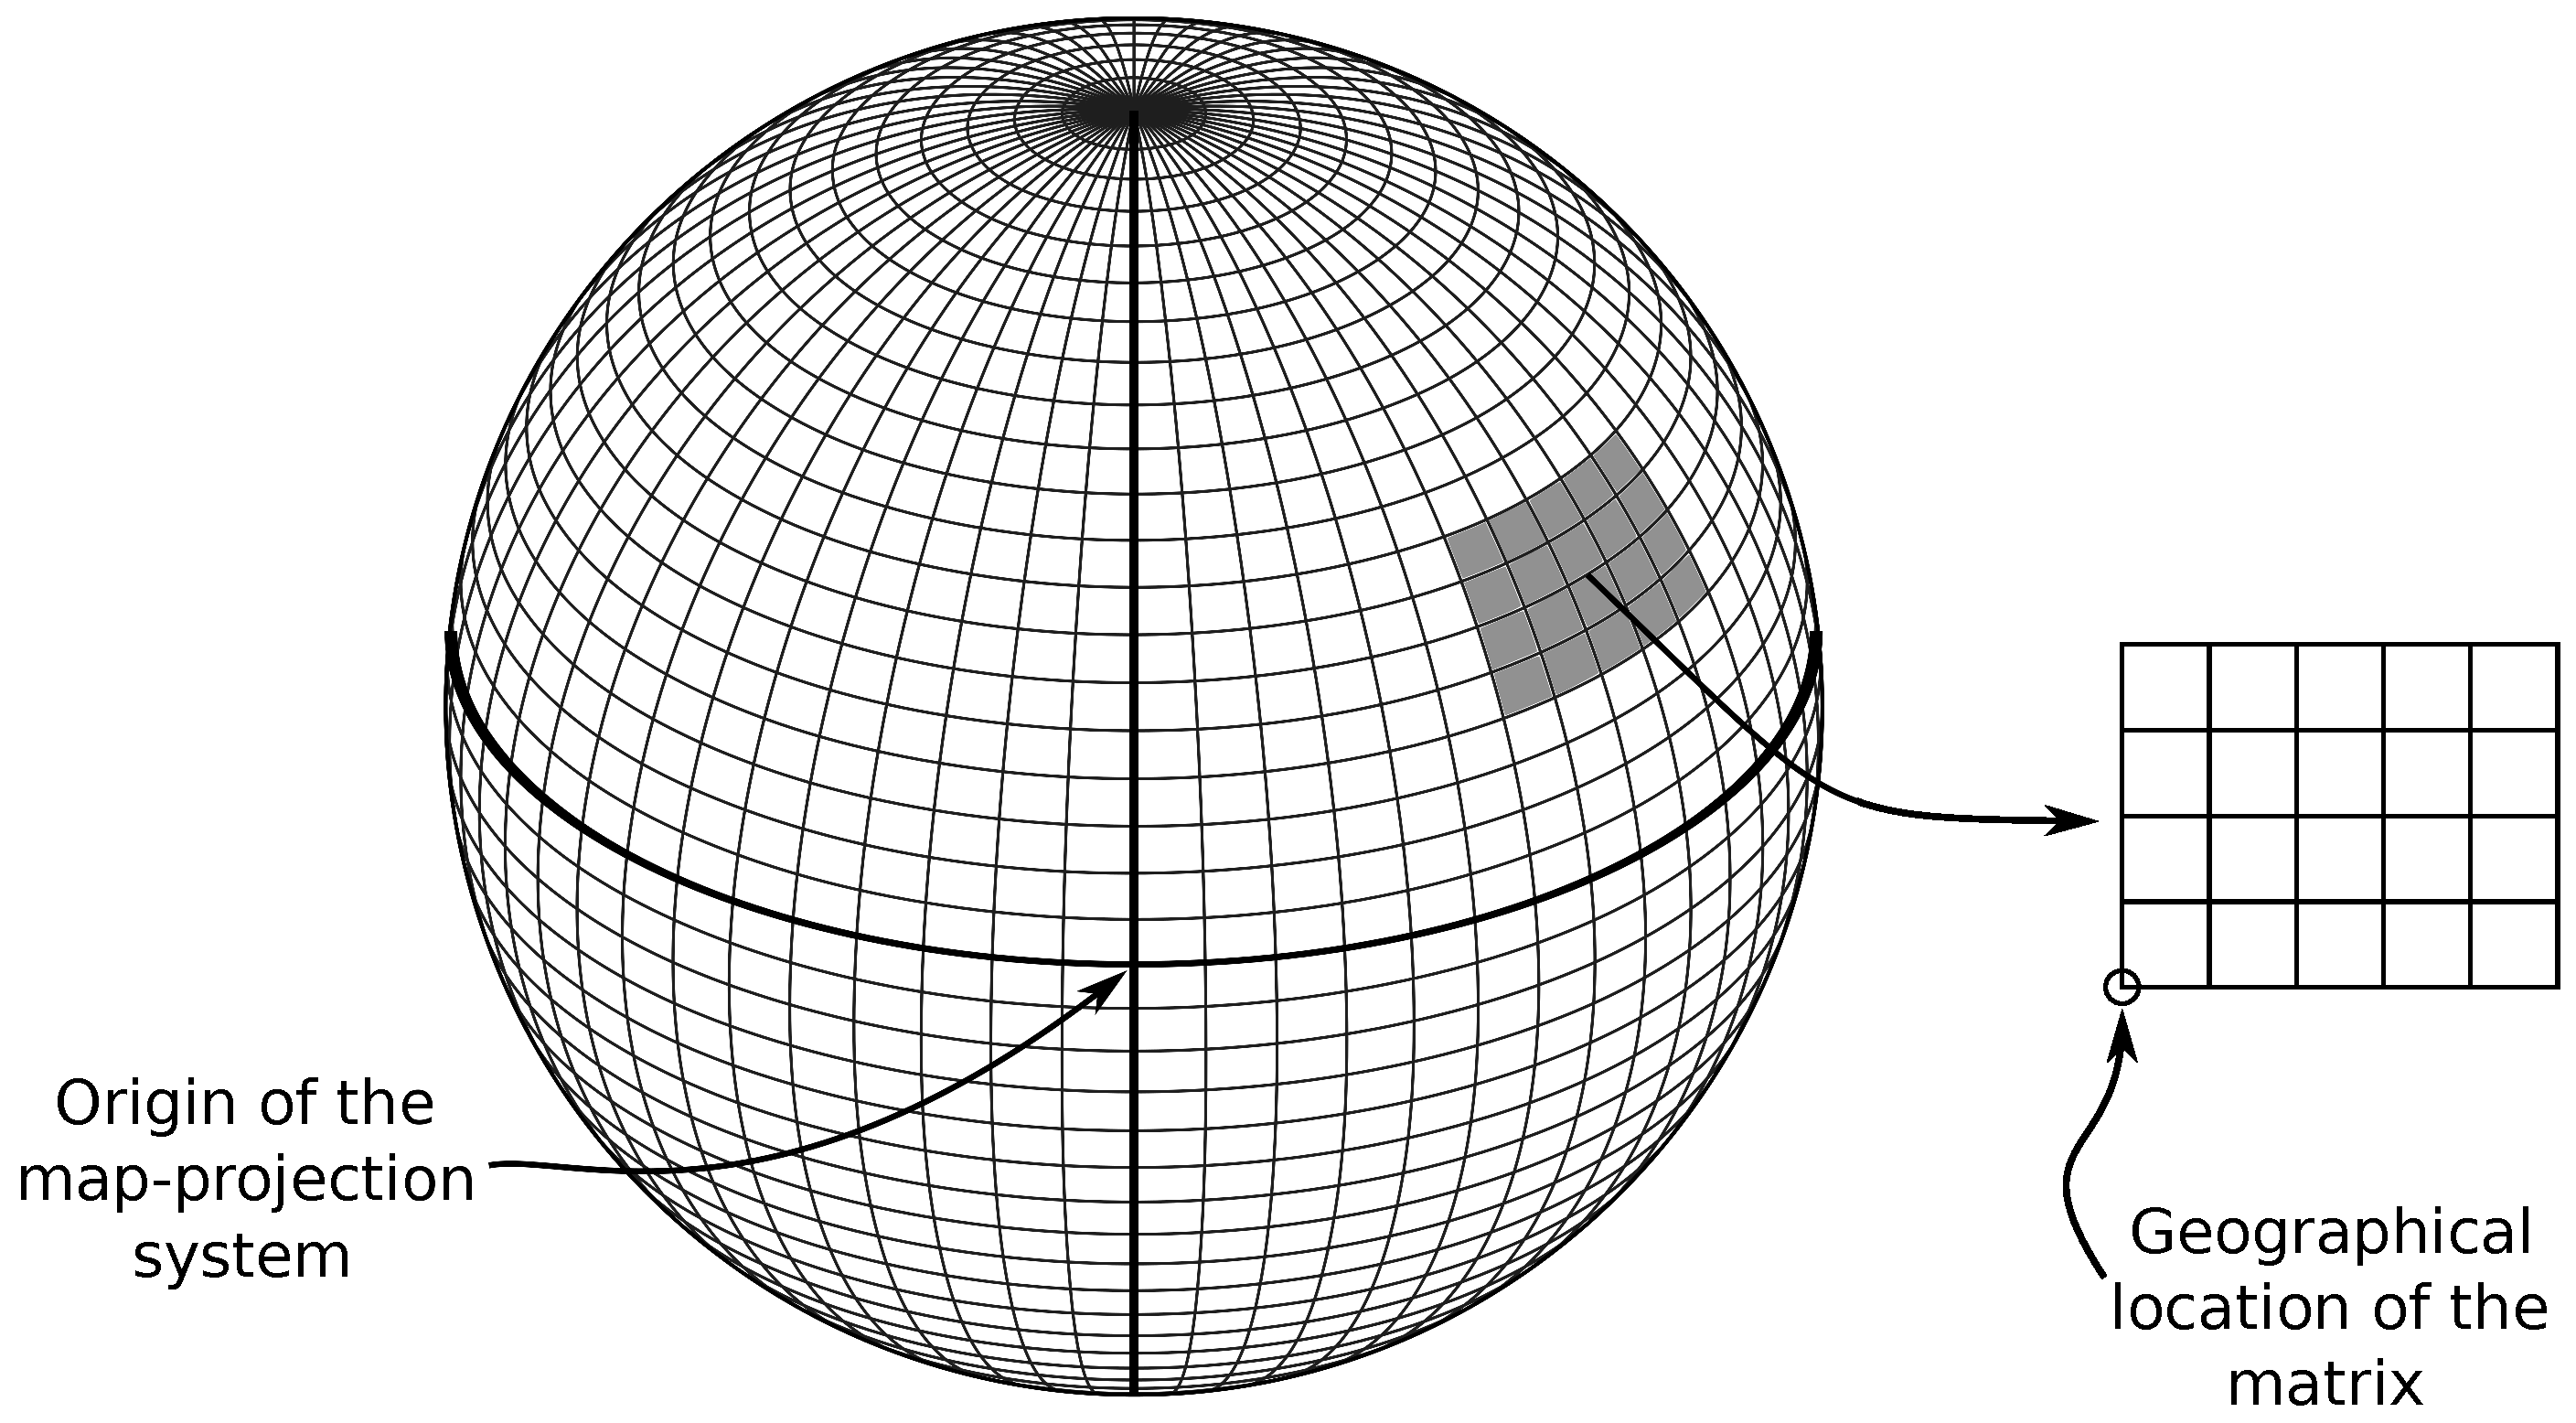
\includegraphics[width=1\textwidth]{04-framework_design_and_implementation/img/spatial_data_projection}

\caption{Example of a geographical-location mapping of the input-spatial data
into a 2D matrix, the lower-left corner of which indicates the nearest
point to the origin of the map-projection system.\label{fig:04-Spatial_data_location_mapping}}
\end{figure}


In the area of geographical-information science, the master-worker
paradigm has been successfully applied by several authors~\cite{Akhter-GRASS_GIS_on_high_performance_computing_with_MPI_OpenMP_and_Ninf-G:2010,Akhter_Porting_GRASS_raster_module_to_distributed_computing:2007,Campos_Parallel_modelling_in_GIS:2012,Guan_A_parallel_computing_approach_to_fast_geostatistical_areal_interpolation:2011,Huang-Explorations_of_the_implementation_of_a_parallel_IDW_algorithm_in_a_Linux_cluster:2011,Tabik-High_performance_three_horizon_composition_algorithm_for_large_scale_terrains:2011,Tabik-Optimal_tilt_and_orientation_maps_a_multi_algorithm_approach_for_heterogeneous_multicore_GPU_systems:2013}.
However, this technique presents certain issues that prevent the full
exploitation of the available computing resources when deployed over
several networked computers. Specifically, the problem refers to network
saturation and idle processes within the master-worker model. Generally
speaking, a single communicating process, e.g., the master, is usually
not able to saturate the network connection of a node. Using more
than one MPI process per node might solve this problem, but possible
rank-ordering problems may appear, thus restricting the full utilization
of the network~\cite{Rabenseifner-Hybrid_MPI_OpenMP_parallel_programming_on_clusters_of_multicore_nodes:2009}.
Additionally, the hardware-exploitation level is difficult to measure
when the parallelization involves only one computing node~\cite{Tabik-High_performance_three_horizon_composition_algorithm_for_large_scale_terrains:2011,Tabik-Optimal_tilt_and_orientation_maps_a_multi_algorithm_approach_for_heterogeneous_multicore_GPU_systems:2013}
(because no network communication is required), or only a few processes
deployed over a handful of nodes~\cite{Huang-Explorations_of_the_implementation_of_a_parallel_IDW_algorithm_in_a_Linux_cluster:2011}. 

Another issue appears when the master process executes the MPI code,
in which case other processes sleep, making a serial use of the communication
component of the system. Consequently, the master process becomes
the bottleneck of the parallel implementation as the number of worker
processes grows. This situation is also common when dealing with the
metadata of a spatial region, which may relate to several elements
of a RSG, making it a frequent cause of load imbalance~\cite{Gong_Parallel_agent_based_simulation_of_individual_level_spatial_interactions_within_a_multicore_computing_environment:2012,Hawick_Distributed_frameworks_and_parallel_algorithms_for_processing_large_scala_geographic_data:2003,Widener_Developing_a_parallel_computational_implementation_of_AMOEBA:2012}.
In PRATO, the transmitter configuration and its antenna diagram represent
metadata that are complementary to the sub-region that a transmitter
covers.

Hybrid MPI-OpenMP implementations~\cite{Tabik-High_performance_three_horizon_composition_algorithm_for_large_scale_terrains:2011,Tabik-Optimal_tilt_and_orientation_maps_a_multi_algorithm_approach_for_heterogeneous_multicore_GPU_systems:2013},
in which no MPI calls are issued inside the OpenMP-parallel regions,
also fail to saturate the network~\cite{Rabenseifner-Hybrid_MPI_OpenMP_parallel_programming_on_clusters_of_multicore_nodes:2009}.
A possible solution to this problem is to improve the communication
overlap among the processes. To this end, PRATO features non-blocking
point-to-point MPI operations, and an independent thread in the worker
process that saves the intermediate results into a DB. One such database
system per computer cluster is used, which also serves the input data
to the GRASS, in order to aggregate the partial results of the path-loss
predictions or to visualize them. It is important to note that any
kind of DB may be used, e.g., relational, distributed~\cite{Ozsu_Principles_of_distributed_database_systems:2011}
or even those of the NoSQL type~\cite{Stonebraker_SQL_databases_vs_NoSQL_databases:2010}.
Nevertheless, a central, relational-database system is used here,
since they are the most popular and widely available ones. Additionally,
the non-blocking message-passing technique used to distribute the
work-load among the nodes provides support for heterogeneous environments.
As a result, computing nodes featuring more capable hardware receive
more work than those with weaker configurations, thus ensuring a better
utilization of the available computing resources despite hardware
diversity, and improved load balancing.


\subsubsection{Master process \label{sub:04-Master-process}}

\begin{figure}
\begin{minipage}[t]{0.49\textwidth}%
\centering

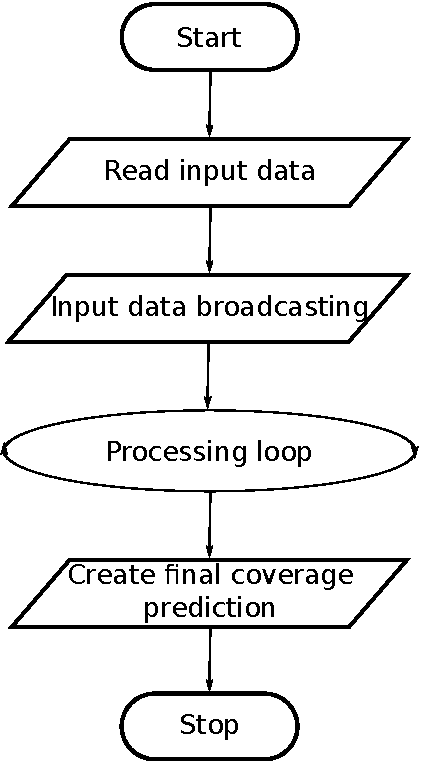
\includegraphics[width=0.55\columnwidth]{04-framework_design_and_implementation/img/master_process_flow_diagram}

\caption{\textit{\emph{Flow diagram of the master process.\label{fig:04-Master_process_flow_diagram}}}}
%
\end{minipage}\hfill{}%
\begin{minipage}[t]{0.49\textwidth}%
\centering


\includegraphics[width=1\columnwidth]{04-framework_design_and_implementation/img/master_processing_loop_flow_diagram}

\caption{\textit{\emph{Flow diagram of the ``Processing loop'' step of the
master process.\label{fig:04-Processing_loop_in_master_process}}}}
%
\end{minipage}
\end{figure}


The master process, the flow diagram of which is given in Figure~\ref{fig:04-Master_process_flow_diagram},
is the only component that runs within the GRASS environment. As soon
as the master process starts, the input parameters are read. This
step corresponds to ``Read input data'' in Figure~\ref{fig:04-Master_process_flow_diagram},
and it is carried out in a similar way as in the serial version. The
next step delivers the metadata that is common to all the transmitters
to all the processes (see ``Metadata broadcasting'' in Figure~\ref{fig:04-Master_process_flow_diagram}).
Before distributing the work among the worker processes, the master
process proceeds to decompose the loaded raster data into 2D matrices
of basic-data-type elements, e.g., \emph{float} or \emph{double},
before dispatching them to the multiple worker processes. In this
case, the decomposition applies to the DEM and the clutter data only,
but it could be applied to any point-based data set. In the next step,
the master process starts an asynchronous message-driven processing
loop (see ``Processing loop'' in Figure~\ref{fig:04-Master_process_flow_diagram}),
the main task of which is to assign and distribute the sub-region
and configuration data of different transmitters among the idle worker
processes.

The flow diagram shown in Figure~\ref{fig:04-Processing_loop_in_master_process}
illustrates the ``Processing loop'' step of the master process.
In the processing loop, the master process starts by checking the
available worker processes that might calculate the radio-coverage
prediction for the next transmitter. It is worth pointing out that
this step also serves as a stopping condition for the processing loop
itself (see ``Any worker still on?'' in Figure~\ref{fig:04-Processing_loop_in_master_process}).
The active worker processes inform the master process that they are
ready to compute by sending an idle message (see ``Wait for idle
worker'' in Figure~\ref{fig:04-Processing_loop_in_master_process}).
The master process then announces to the idle worker process that
it is about to receive new data for the next calculation, and it dispatches
the complete configuration of the transmitter to be processed (see
``Send keep-alive message'' and ``Send transmitter data'' steps,
respectively, in Figure~\ref{fig:04-Processing_loop_in_master_process}).
This is only done in the case that there are transmitters for which
the coverage prediction has yet to be calculated (see ``Any transmitters
left?'' in Figure~\ref{fig:04-Processing_loop_in_master_process}).
The processing loop of the master process continues distributing the
transmitter data among the worker processes, which asynchronously
become idle as they finish the radio-prediction calculations they
have been assigned by the master process. When there are no more transmitters
left, all the worker processes announcing they are idle will receive
a shutdown message from the master process, indicating to them that
they should stop running (see ``Send stop message'' in Figure~\ref{fig:04-Processing_loop_in_master_process}).
The master process will keep doing this until all the worker processes
have finished (see ``Any worker still on?'' in Figure~\ref{fig:04-Processing_loop_in_master_process}),
thus fulfilling the stopping condition of the processing loop.

Finally, the last step of the master process is devoted to creating
the final output of the calculation, e.g., a raster map (see ``Create
final coverage prediction'' in Figure~\ref{fig:04-Master_process_flow_diagram}).
The final coverage prediction of all the transmitters is an aggregation
from the individual path-loss results created by each of the worker
processes during the ``Processing loop'' phase in Figure~\ref{fig:04-Master_process_flow_diagram},
which provides the source data for the final raster map. The aggregation
of the individual path-loss results is accomplished by issuing an
SQL query over the database tables containing them, in a similar way
as in the serial version.


\subsubsection{Worker processes on CPU}

An essential characteristic of the worker processes is that they are
completely independent of the GRASS, i.e., they do not have to run
within the GRASS environment nor use any of the GRASS libraries to
work. This aspect significantly simplifies the deployment phase to
run PRATO on a computer cluster, since no GRASS installation is needed
on the computing nodes hosting the worker processes.

One possibility to overcome the thread-safety limitation of the GRASS
is to save the transmitter path-loss predictions through the master
process, thus avoiding concurrent access. However, for the workers
to send intermediate results back to the master process, e.g., as
in~\cite{Akhter-GRASS_GIS_on_high_performance_computing_with_MPI_OpenMP_and_Ninf-G:2010,Huang-Explorations_of_the_implementation_of_a_parallel_IDW_algorithm_in_a_Linux_cluster:2011},
is a major bottleneck for the scalability of a parallel implementation.
In such case, the scalability is limited by the master process, because
it must serially process the received results in order to avoid inconsistencies
due to concurrent access. Instead, PRATO allows each of the worker
processes to output its intermediate results into a DB, i.e., each
path-loss prediction in its own table. Additionally, worker processes
do this from an independent thread, which runs concurrently with the
calculation of the next transmitter received from the master process.
In this way, the overlap between the calculation and communication
significantly hides the latency created by the result-dumping task,
thus making better use of the available system resources.

The computations of the worker processes, the flow diagram of which
is given in Figure~\ref{fig:04-Worker_process_flow_diagram}, begin
by receiving metadata about the transmitters and the geographical
area from the master process during the initialization time (see ``Receive
broadcasted metadata'' in Figure~\ref{fig:04-Worker_process_flow_diagram}).

After the broadcasted metadata are received by all the worker processes,
each one proceeds to inform the master process that it is ready (i.e.,
in an idle state) to receive the transmitter-configuration data that
define which transmitter path-loss prediction to perform (see ``Send
idle message'' in Figure~\ref{fig:04-Worker_process_flow_diagram}).
If the master process does not give the instruction to stop processing
(see ``Has stop message arrived?'' in Figure~\ref{fig:04-Worker_process_flow_diagram}),
the worker process collects the sub-region spatial data and the transmitter
configuration (see ``Receive transmitter data'' in Figure~\ref{fig:04-Worker_process_flow_diagram}).
In the event that a stop message is received, the worker process will
wait for any result-dumping thread to finish (see ``Wait for result-dump
thread'' in Figure~\ref{fig:04-Worker_process_flow_diagram}) before
shutting down. The coverage calculation itself follows a similar design
as the serial version (see ``Coverage calculation'' in Figure~\ref{fig:04-Worker_process_flow_diagram}).

As mentioned before, the worker process launches an independent thread
to save the path-loss prediction of the target transmitter into a
DB table (see ``Threaded save path-loss to DB'' in Figure~\ref{fig:04-Worker_process_flow_diagram}).
It is important to note that there is no possibility of data inconsistency
due to the saving task being executed inside a thread, since path-loss
data from different workers belong to different transmitters and are,
at this point of the process, mutually exclusive.

\begin{figure}
\begin{minipage}[t]{0.49\textwidth}%
\centering

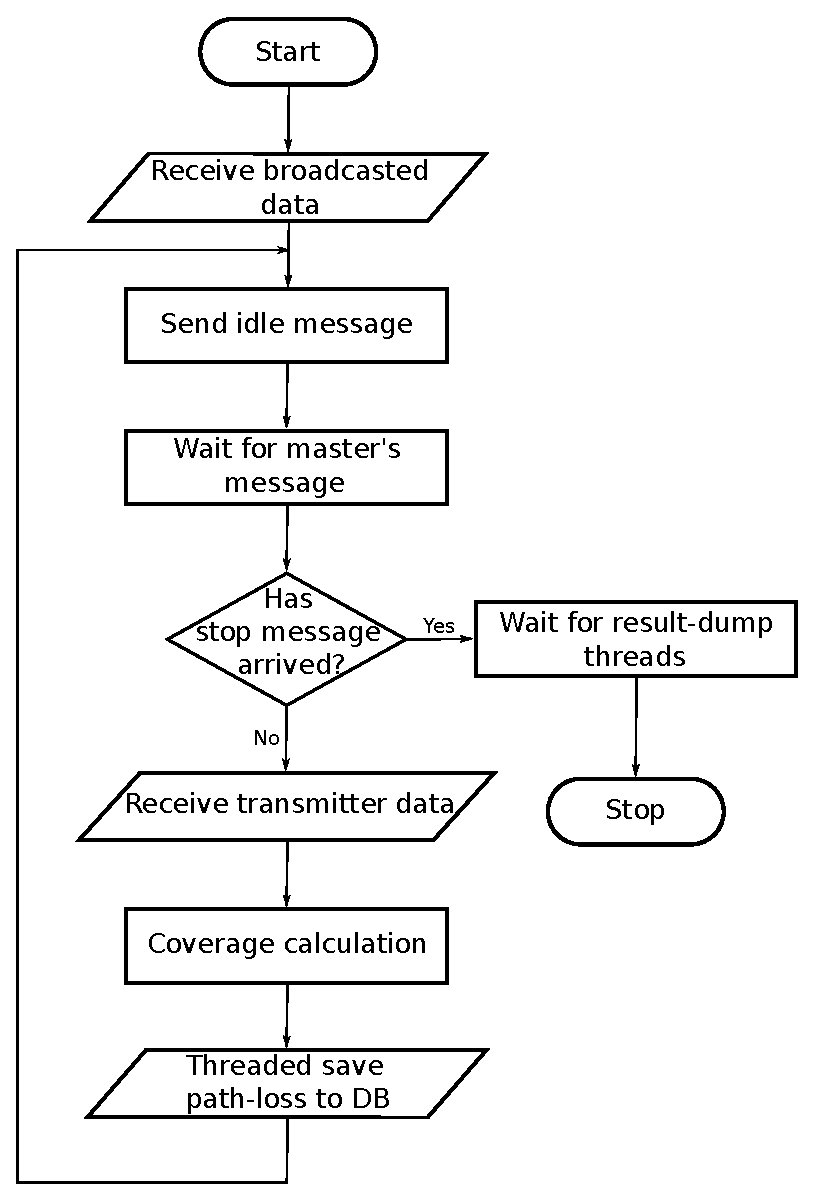
\includegraphics[width=0.9\columnwidth]{04-framework_design_and_implementation/img/worker_process_flow_diagram}

\caption{\textit{\emph{Flow diagram of a worker process.\label{fig:04-Worker_process_flow_diagram}}}}
%
\end{minipage}\hfill{}%
\begin{minipage}[t]{0.49\textwidth}%
\centering

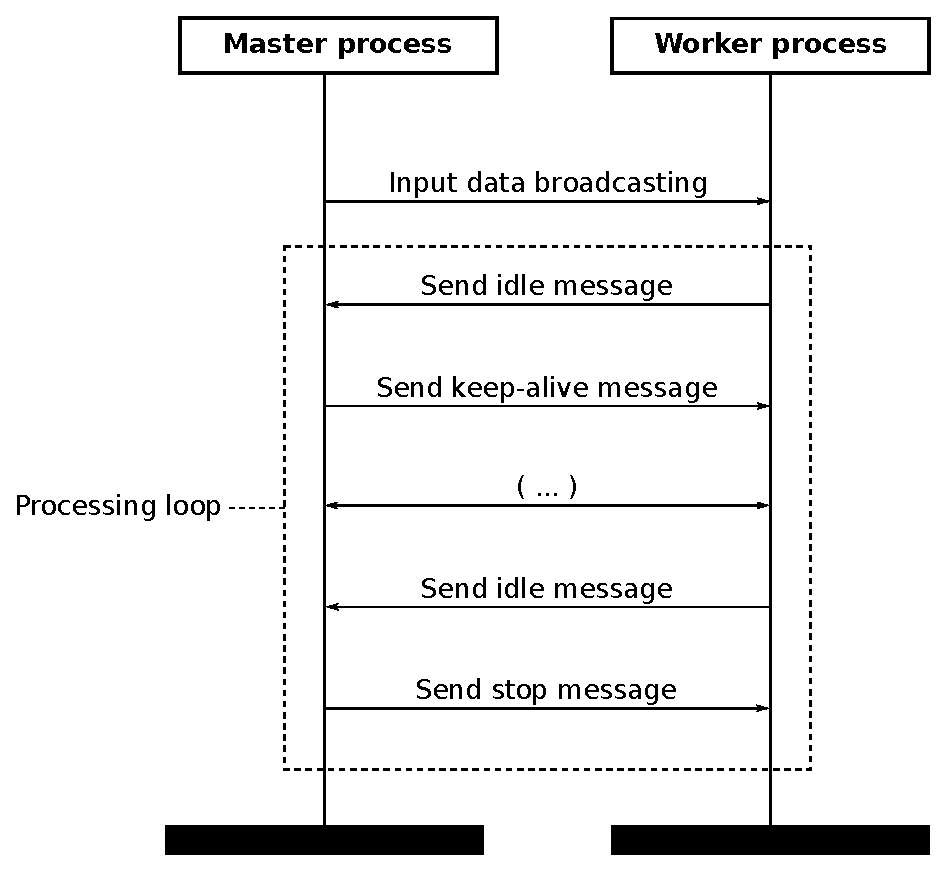
\includegraphics[width=1\columnwidth]{04-framework_design_and_implementation/img/master_worker_communication_diagram}

\caption{\textit{\emph{Communication diagram, showing the message passing between
the master and a worker process.\label{fig:04-Master_worker_communication}}}}
%
\end{minipage}
\end{figure}



\subsubsection{Worker processes on GPU \label{sub:04-GPU_worker_implementation}}

PRATO provides multi-GPU support for improving the execution performance
on the computing nodes hosting the worker processes. The algorithmic
adaptation from a CPU to a GPU is not a trivial task. This section
focuses on the main modifications made to the radio-propagation algorithm
in order for it to work on GPU hardware.

It is well known that the bandwidth of the PCI Express bus can cause
a throughput bottleneck when a significant amount of data is transferred
between a CPU and a GPU in a heterogeneous system~\cite{Gregg-Where_is_the_data:2011}.
Some researchers acknowledged that unless a full working set of data
can fit into the memory on a GPU, the PCI Express will become the
bottleneck of the system~\cite{Owens-GPU_computing:2008,Schaa-Exploring_the_multiple_GPU_design_space:2009}.
For this reason, it is imperative to have as much data as possible
allocated on the GPU itself.

In order to minimize the CPU-to-GPU memory transfers, the spatial
data used by the radio-propagation algorithm was organized as explained
in Section~\ref{sub:04-Design_of_the_parallel_version}, i.e., using
geographically-located, offset-based 2D matrices. However, the internal
representation of the matrix elements was changed to use less memory.
To this end, the clutter-matrix elements were represented as \emph{unsigned
char}, since they express signal loss in dB. It follows that for the
radio-propagation prediction of one transmitter, the following matrices
should be allocated on the GPU:
\begin{itemize}
\item one 2D matrix containing DEM data for the target subregion, the elements
of which are \emph{float} or \emph{double}; 
\item one 2D matrix containing clutter data for the target subregion, the
elements of which are \emph{unsigned char}; and
\item one 2D matrix containing the resulting path-loss prediction.
\end{itemize}
The dimension of all matrices is based on the transmission radius,
within which the radio-propagation prediction should be calculated.
The contents of the DEM and clutter matrices is constant throughout
the calculation process. For this reason they were kept in texture
memory to take advantage of the faster access time (see Section~\ref{sec:02-CUDA}).
Regarding the resulting path-loss matrix, each step of the radio-prediction
algorithm is applied over the results of the previous step (see Figure~\ref{fig:04-Flow_diagram_serial_version}
for a flow diagram of the steps involved), thus avoiding extra allocation
on global memory or a data-transfer from/to the CPU.


\subsubsection{Master-worker communication}

Similar to~\cite{Tabik-High_performance_three_horizon_composition_algorithm_for_large_scale_terrains:2011,Tabik-Optimal_tilt_and_orientation_maps_a_multi_algorithm_approach_for_heterogeneous_multicore_GPU_systems:2013},
the message-passing technique used in this work enables a better use
of the available computing resources, both in terms of scalability
and load balancing, while introducing a negligible overhead. This
last point is supported by the experimental results, introduced in
Section~\ref{sub:04-Strong_scalability}.

The first reason to implement the message-passing technique is to
support heterogeneous computing environments. In particular, our approach
focuses on taking full advantage of the hardware of each computing
node, thus explicitly avoiding the bottlenecks introduced by the slowest
computing node in the cluster. This problem appears when evenly distributing
the data among the worker processes on disparate hardware, e.g., as
in~\cite{Akhter_Porting_GRASS_raster_module_to_distributed_computing:2007,Huang-Explorations_of_the_implementation_of_a_parallel_IDW_algorithm_in_a_Linux_cluster:2011},
being more noticeable with a larger number of computing nodes and
processes. In other words, computing nodes that deliver better performance
have more calculations assigned to them. Moreover, in real-world scenarios,
it is often the case that a large number of dedicated computing nodes
featuring exactly the same configuration is difficult to find, i.e.,
not every organization owns a computer cluster.

A second reason for selecting a message-passing technique is related
to the flexibility it provides for load balancing, which is of greater
importance when dealing with extra data or information besides spatial
data~\cite{Hawick_Distributed_frameworks_and_parallel_algorithms_for_processing_large_scala_geographic_data:2003}.
This can be seen in Figure~\ref{fig:04-Processing_loop_in_master_process},
where the master process, before delivering the spatial subset and
transmitter-configuration data, sends a message to the worker process,
indicating that it is about to receive more work. This a-priori meaningless
message plays a key role in correctly supporting the asynchronous
process communication. Notice that the subset of spatial data that
a worker process receives is directly related to the transmitter for
which the prediction will be calculated. Similar to~\cite{Tabik-High_performance_three_horizon_composition_algorithm_for_large_scale_terrains:2011,Tabik-Optimal_tilt_and_orientation_maps_a_multi_algorithm_approach_for_heterogeneous_multicore_GPU_systems:2013},
this problem-specific property enables the use of a data-decomposition
technique based on a block partition of spatial data, e.g., the DEM
and clutter data.

In general, there are many different ways a parallel program can be
executed, because the steps from the different processes can be interleaved
in various ways and a process can make non-deterministic choices~\cite{Siegel_Verification_of_halting_properties_for_MPI_programs:2007},
which may lead to situations such as race conditions~\cite{Clemencon_MPI_Race_detection:1995}
and deadlocks. A deadlock occurs whenever two or more running processes
are waiting for each other to finish, and thus neither ever does.
To prevent PRATO from deadlocking, message sending and receiving should
be paired, i.e., an equal number of send and receive messages on the
master and worker sides~\cite{Siegel_Verification_of_halting_properties_for_MPI_programs:2007}.
Figure~\ref{fig:04-Master_worker_communication} depicts the master-worker
message passing, from which the transmitter-data transmission has
been excluded for clarity. Notice how each idle message sent from
the worker process is paired with an answer from the master process,
whether it is a keep-alive or a stop message.


\section{Simulations \label{sec:04-Simulations}}

Considering the large computational power needed for predicting the
radio-coverage of a real radio network, the use of a computer cluster
is recommended. A computer cluster is a group of interconnected computers
that work together as a single system. Computer clusters typically
consist of several commodity PCs connected through a high-speed local-area
network (LAN\nomenclature[A]{LAN}{Local area network}) with a distributed
file system, like the network file system (NFS\nomenclature[A]{NFS}{Network file system})~\cite{Shepler_Network_file_system:2003}.
One such system is the DEGIMA cluster \cite{Hamada_Cluster_of_GPUs:2010}
at the Nagasaki Advanced Computing Center (NACC\nomenclature[A]{NACC}{Nagasaki advanced computing center})
of the Nagasaki University in Japan. This system ranked in the TOP
500 list of supercomputers until June 2012%
\footnote{http://www.top500.org%
}, and in June 2011 it held the third place in the Green 500 list%
\footnote{http://www.green500.org%
} as one of the most energy-efficient supercomputers in the world.

This section presents the simulations, and an exhaustive analysis
of the performance and scalability of the parallel implementation
of PRATO. The most common usage case for PRATO is to perform a radio-coverage
prediction for multiple transmitters. Therefore, a straight-forward
parallel decomposition is to divide a given problem instance by transmitter,
for which each coverage prediction is calculated by a separate worker
process.

The following simulations were carried out on 34 computing nodes of
the DEGIMA cluster. The computing nodes are connected by a LAN, over
a Gigabit Ethernet interconnect. As mentioned before, the reason for
using a high-end computer cluster such as DEGIMA is to explore, by
experimentation, the advantages and drawbacks of the considered methods.
However, this does not imply any loss of generality if applying these
principles over a different group of networked computers that do not
operate as a computer cluster. Moreover, PRATO also supports parallel
calculation of radio-propagation predictions for multiple cells by
distributing the processes among the individual cores of a single
CPU.

Each computing node of DEGIMA features one of two possible configurations,
namely:
\begin{itemize}
\item Intel Core i5-2500T quad-core processor CPU, clocked at 2.30 GHz,
with 16 GB of RAM; and
\item Intel Core i7-2600K quad-core processor CPU, clocked at 3.40 GHz,
also with 16 GB of RAM.
\end{itemize}
During the simulation runs, the nodes equipped with the Intel i5 CPU
hosted the worker processes, whereas the master process and the PostgreSQL
database server (version 9.1.4) each run on a different computing
node, featuring an Intel i7 CPU. The DB server performed all its I/O
operations on the local file system, which was mounted on an 8~GB
RAM disk. During the simulations, the path-loss predictions of 5,120
transmitters occupied less than 4~GB of this partition. No GPU hardware
was used for the following simulation sets.

A 64-bit Linux operating system (Fedora distribution) was the operating
system used. The message-passing implementation OpenMPI, version 1.6.1,
was manually compiled with the distribution-supplied gcc compiler,
version 4.4.4.


\subsection{Test networks}

The parallel performance of PRATO was tested with real radio networks
of different sizes. In order to create the synthetic test data sets
with an arbitrary number of transmitters, a group of 2,000 transmitters
of a real network was used. The configuration parameters of these
transmitters resembled those of the LTE network deployed in Slovenia
by Telekom Slovenije, d.d., which were, in turn, randomly replicated
and distributed over the whole target area. The path-loss predictions
were calculated using the radio-propagation model introduced in Section~\ref{sub:04-Radio_propagation_model}.
The DEM area, as well as the clutter data, covered 20,270~km$^{2}$
with a pixel resolution of 25~m$^{2}$. The clutter data contained
different levels of signal loss due to land usage. For all the points
within a radius of 20~km around each transmitter, a receiver positioned
1.5~m above the ground was assumed, and the frequency was set to
1,843~MHz.


\subsection{Weak scalability}

The weak-scalability experiments are meant to analyze the scalability
of the parallel implementation in cases where the workload assigned
to each process (one MPI process per processor core) remains constant
as the number of processor cores is increased. It follows that the
number of transmitters deployed over the target area is directly proportional
to the number of processor cores and worker processes. This was accomplished
by assigning a constant number of transmitters per core, while increasing
the number of cores hosting the worker processes. Here, the following
numbers of transmitters per worker/core were tested \{5,~10,~20,~40,~80\},
by progressively doubling the number of worker processes from 1 to
64.

Problems that are particularly well-suited for parallel computing
exhibit computational costs that are linearly dependent on the size
of the problem. This property, also referred to as algorithmic scalability,
means that proportionally increasing both the problem size and the
number of cores results in a roughly constant time to solution.

The master-worker (MW\nomenclature[A]{MW}{Master-worker parallel paradigm})
configuration performs result aggregation continuously, i.e., while
receiving the intermediate results from the worker processes. In contrast,
the master-worker-DB (MWD\nomenclature[A]{MWD}{Master-worker-database parallel paradigm})
setup performs the result aggregation as the final step. This set
of experiments is meant to investigate how the proposed MWD technique
compares with the classic MW approach in terms of scalability when
dealing with a constant computational load per core.

An important fact about the presented simulations when using multi-threaded
implementations is to avoid oversubscribing a computing node. For
example, if deploying four worker processes over a quad-core CPU,
the extra threads will have a counter effect on the parallel efficiency,
since the CPU resources would be exhausted, which slows the whole
process down. For this reason, we have deployed three worker processes
per computing node, leaving one core free for executing the extra
threads. 


\subsubsection*{Results}

The results represent the average running time out of a set of 20
independent simulation runs, for which the transmitters and the rank
ordering of the worker processes were randomly selected. The collected
running times for the weak-scalability experiments are shown in Figure~\ref{fig:04-Weak_scalability_time}.
All the measurements express wall-clock times in seconds for each
setup and problem instance, defined as the number of transmitters
per process (Tx/process). The wall-clock time represents the real
time that elapses from the start of the master process to its end,
including the time that passes while waiting for the resources to
become available. The running-time improvements of the MWD versus
the MW setup are shown in Table~\ref{tab:04-Weak_scaling-time_gain}.

\begin{figure}
\centering

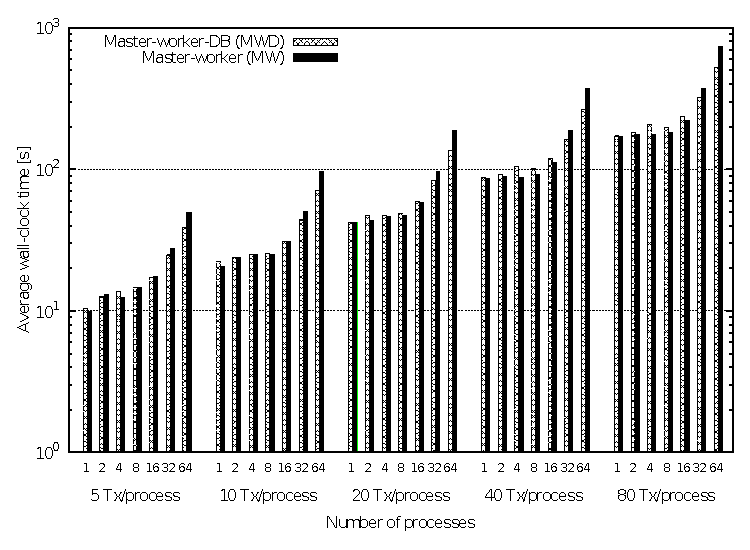
\includegraphics[width=0.8\textwidth]{04-framework_design_and_implementation/img/weak_scaling-time_plot}

\caption{\textit{\emph{Measured wall-clock time for weak-scalability experiments,
featuring MW and MWD setups.}}\textit{ }\textit{\emph{Experiments
allocated one MPI worker process per core.\label{fig:04-Weak_scalability_time}}}}
\end{figure}


\begin{table}
\centering

\caption{\textit{\emph{Running-time gain (in percent) of the simulations for
the weak-scalability of the MWD setup relative to the classic MW approach.\label{tab:04-Weak_scaling-time_gain}}}}


{\small{}}%
\begin{tabular}{cccccccc}
\cmidrule{2-8} 
 & \multicolumn{7}{c}{{\small{Number of cores}}}\tabularnewline\addlinespace
\midrule 
{\small{TX/core}} & {\small{1}} & {\small{2}} & {\small{4}} & {\small{8}} & {\small{16}} & {\small{32}} & {\small{64}}\tabularnewline
\midrule
{\small{5}} & {\small{-11.39}} & {\small{-10.42}} & {\small{-11.14}} & {\small{-0.95}} & {\small{11.75}} & {\small{26.15}} & {\small{32.53}}\tabularnewline
{\small{10}} & {\small{-5.84}} & {\small{-7.78}} & {\small{-7.67}} & {\small{0.91}} & {\small{12.81}} & {\small{33.28}} & {\small{33.55}}\tabularnewline
{\small{20}} & {\small{-8.59}} & {\small{-10.88}} & {\small{-1.04}} & {\small{1.95}} & {\small{14.29}} & {\small{35.23}} & {\small{35.27}}\tabularnewline
{\small{40}} & {\small{-5.26}} & {\small{-6.90}} & {\small{-3.68}} & {\small{-0.67}} & {\small{17.27}} & {\small{36.23}} & {\small{36.65}}\tabularnewline
{\small{80}} & {\small{-5.29}} & {\small{-7.11}} & {\small{-3.20}} & {\small{-0.31}} & {\small{17.94}} & {\small{36.32}} & {\small{36.57}}\tabularnewline
\bottomrule
\end{tabular}
\end{table}


The time measurements observed from the weak-scalability results show
that the classic MW approach performs well for up to four worker processes.
When using eight worker processes, the MW setup is practically equivalent
to the MWD approach, indicating that the master process is being fully
exploited. When increasing the problem size and the number of worker
processes to 16, the running-time gain is already clear, favoring
the MWD configuration. This gain keeps growing, although slower, as
we increase the number of worker processes to 32 and 64, confirming
the hypothesis that in a classic MW approach, the parallel efficiency
is bounded by the capacity of the master process to serve an increasing
number of worker processes. Interestingly, the gain when using 32
and 64 worker processes is almost the same. After further investigation,
the reason for this behavior was found: the new bottleneck was the
LAN being completely saturated by the worker processes. Consequently,
they have to wait for the network resources to become available before
sending or receiving data, which is not the case when running the
MW setup. Therefore, using the MWD approach a hardware constraint
is hit, meaning that the bottleneck is no longer at the implementation
level. Moreover, since the master process is far from overloaded when
serving 64 worker processes, it can be expected that the MWD approach
will keep scaling if a faster network infrastructure is used, e.g.,
10-gigabit Ethernet or InfiniBand.

Certainly, the parallel version of PRATO scales better using the MWD
approach, when challenged with a large number of transmitters (5,120
for the biggest instance) over 64 cores. This fact shows PRATO would
be able to calculate the radio-coverage prediction for real networks
in a feasible amount of time, since many operational radio networks
have already deployed a comparable number of transmitters, e.g., the
3G network within the Greater London Authority area, in the UK~\cite{Number_of_base_stations_in_England}.
For a more in-depth discussion and experimentation about real-world
planning scenarios, see Chapter~\ref{chap:08-Real-world_network_planning}.

Not being able to achieve perfect weak scalability using the MWD setup
is due to a number of factors. Specifically, the overhead time of
the serial sections of the parallel process grows proportionally with
the number of cores, e.g., aggregation of the intermediate results,
although the total contribution of this overhead remains low for large
problem sizes. Moreover, the communication overhead grows linearly
with the number of cores used. Consequently, the findings of Huang
et al. \cite{Huang-Explorations_of_the_implementation_of_a_parallel_IDW_algorithm_in_a_Linux_cluster:2011}
can be confirmed, who concluded that the data-set size should be large
enough for the communication overhead to be hidden by the calculation
time. This ensures profitable parallelization in terms of running-time
reduction.


\subsection{Strong scalability \label{sub:04-Strong_scalability}}

This set of simulations is meant to analyze the impact of increasing
the number of computing cores for a given problem size, i.e., the
number of transmitters deployed over the target area does not change,
but only the number of worker processes used is increased. Here, the
following number of transmitters were tested \{1,280,~2,560,~5,120\},
by gradually doubling the number of workers from 1 to 64 for each
problem size.


\subsubsection*{Results}

\begin{figure}
\centering

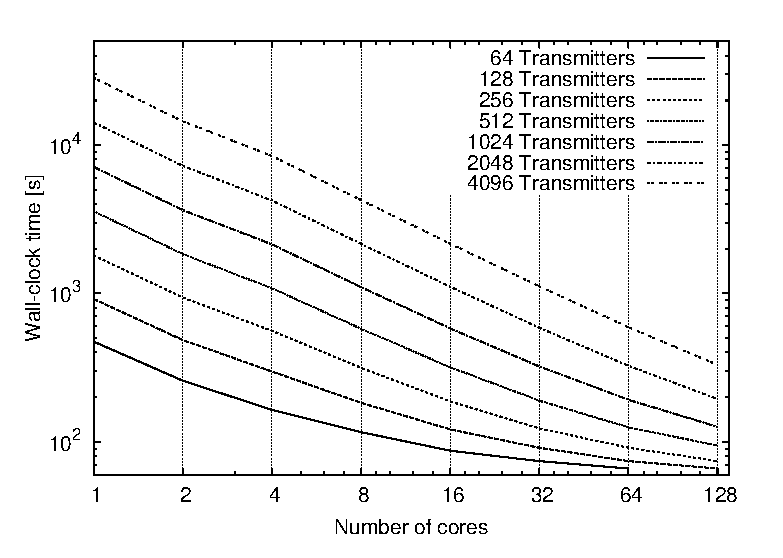
\includegraphics[width=0.8\columnwidth]{04-framework_design_and_implementation/img/strong_scaling-time_plot}

\caption{\textit{\emph{Measured wall-clock time for strong-scalability experiments,
featuring MW and MWD setups.}}\textit{ }\textit{\emph{Experiments
assigned one MPI worker process per core. \label{fig:04-Strong_scalability_time}}}}
\end{figure}


Similar to the weak-scalability experiments, the time measurements
plotted in Figure~\ref{fig:04-Strong_scalability_time} show that,
when applying a classic MW approach, the \textit{\emph{running-time
reduction}} starts flattening if more than eight worker processes
were used. Moreover, the running times for 16, 32 and 64 worker processes
are the same, i.e., they do not improve due to the master process
being \textit{\emph{saturated}}. In contrast, when using the proposed
MWD technique, the running-time reduction improves for up to 32 worker
processes, after which there is no further improvement since the network
was being fully exploited. These results clearly show that when applying
parallelization using a larger number of worker processes, the master
process becomes the bottleneck of the MW approach. When using the
MWD configuration, a steady running-time reduction is observed, until
a hardware constraint is hit, e.g., the network infrastructure.

The overhead of sending/receiving asynchronous messages in order to
support heterogeneous systems was also measured. It was found that
this overhead never exceeds 0.02~\% of the total running time for
the MW experiments, and 0.01~\% for the MWD experimental set.


\subsubsection{Speedup}

In order to further analyze how well the PRATO scales using the MW
and MWD approaches, the performance of the parallel implementation
in terms of its speedup was measured, which is defined as:

\begin{equation}
S(NP)=\frac{execution\, time\, for\, base\, case}{execution\, time\, for\, NP\, cores},\label{eq:04-Speedup}
\end{equation}


\noindent where $NP$ is the number of cores executing the worker
processes. The parallel implementation running on only one core was
the base case for comparisons. The serial implementation is not a
good base comparison for the parallel results as it does not reuse
the resources between each transmitter-coverage calculation and it
does not overlap the I/O operations with the transmitter computations.
In practice, this means that several concatenated runs of the serial
version would be considerably slower than the single-worker configuration.

\begin{figure}
\begin{minipage}[t]{0.48\textwidth}%
\centering

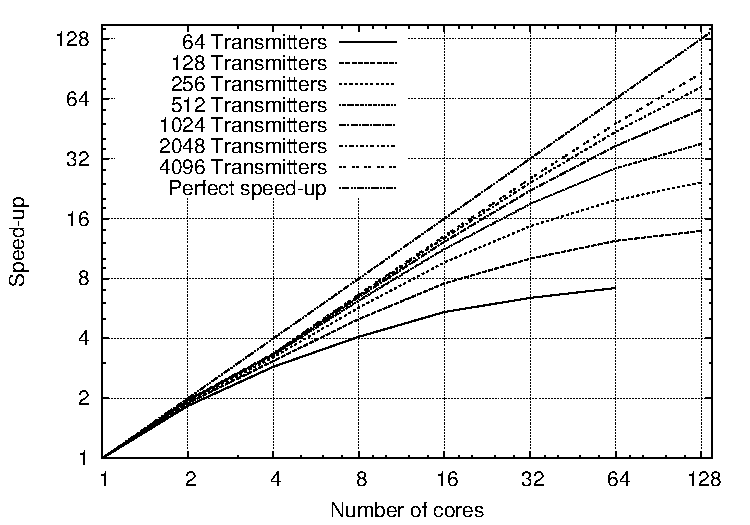
\includegraphics[width=1\columnwidth]{04-framework_design_and_implementation/img/strong_scaling-speedup_plot}

\caption{\textit{\emph{Average speedup for the strong-scalability experiments.
\label{fig:04-Strong_scalability_speedup}}}}
%
\end{minipage}\hfill{}%
\begin{minipage}[t]{0.48\textwidth}%
\centering

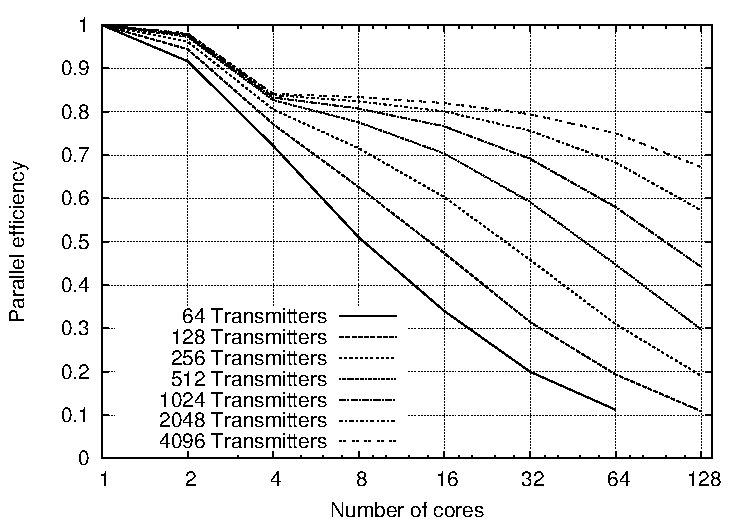
\includegraphics[width=1\columnwidth]{04-framework_design_and_implementation/img/strong_scaling-efficiency_plot}

\caption{\textit{\emph{Average parallel efficiency for the strong-scalability
experiments.}}\textit{ }\textit{\emph{\label{fig:04-Strong_scalability_efficiency}}}}
%
\end{minipage}
\end{figure}


Using the speedup metric, linear scaling is achieved when the obtained
speedup is equal to the total number of processors used. However,
it should be noted that a perfect speedup is almost never achieved,
due to the existence of serial stages within an algorithm and the
communication overhead of the parallel implementation.

Figure~\ref{fig:04-Strong_scalability_speedup} shows the average
speedup of the parallel implementation for up to 64 worker processes,
using the standard MW method and the proposed MWD approach. The average
speedup was calculated for the three different problem instances,
i.e., 1,280, 2,560, and 5,120 transmitters deployed over the target
area. The number of transmitters used in these problem sizes is comparable
to several real-world radio networks that were already deployed in
England, e.g., Hampshire County with 227 BSs, West Midlands with 414
BSs, and Greater London Authority with 1,086 BSs \cite{Number_of_base_stations_in_England}.
Note that it is common for a single base station to host multiple
transmitters. 

The plotted average speedup clearly shows the minimal overhead of
the MWD approach when using a small number of worker processes. This
overhead accounts for the final aggregation of the intermediate results
at the DB, which in the MW configuration is performed along worker
processing. Like before, the DB component allows the parallel implementation
to fully exploit the available computing resources when deploying
a larger number of worker processes, until the network-capacity limit
is met. Of course, these results are directly correlated with the
wall-clock times shown in Figure~\ref{fig:04-Strong_scalability_time}.


\subsubsection{Efficiency}

Another measure to study how well PRATO utilizes the available computing
resources considers the parallel efficiency of the implementation.
The definition of parallel efficiency is as follows:

\begin{equation}
E(NP)=\frac{S(NP)}{NP},
\end{equation}


\noindent where $S(NP)$ is the speedup as defined in Equation~(\ref{eq:04-Speedup}),
and $NP$ is the number of cores executing worker processes. Figure~\ref{fig:04-Strong_scalability_efficiency}
shows the average parallel efficiency of the parallel implementation
for different problem sizes, as the number of processing cores was
increased. Like for the speedup measure, the average parallel efficiency
from the same problem instances was calculated.

The ideal case for a parallel application would be to utilize all
the available computing resources, in which case the parallel efficiency
would always be equal to one as the core count increases. From the
plot in Figure~\ref{fig:04-Strong_scalability_efficiency}, it can
be observed that the efficiency of the MWD approach is better than
in the MW case for larger number of processes, and as long as there
was available capacity at the LAN level. In accordance to the previous
analysis, the under utilization of the computing resources is more
significant when the master process is overloaded (in the MW case)
than when the network infrastructure is saturated (in the MWD case).
The lower efficiency is directly proportional to the number of idle
worker processes that wait either for the master process (MW case)
or for network access (MWD case).

Overall, the experimental results confirm that the objective of fully
exploiting the available hardware resources is accomplished when applying
the presented MWD approach, thus improving the scalability and efficiency
of PRATO when compared to a traditional MW technique.




\section{Summary \label{sec:04-Summary}}

PRATO, a parallel radio-coverage prediction tool for radio networks,
has been presented in this chapter. The tool is intended to be used
for radio-network planning analysis and decision support. Its high-performance
capabilities make it ideal for automatic-optimization tasks that require
a large number of evaluations.

The parallel implementation of PRATO includes a novel parallel technique
for master-worker configurations. The introduced MWD technique, which
combines the use of a DB system with a work-pool approach, delivers
improved performance when compared with a traditional MW setup. Moreover,
the presented system provides parallel and asynchronous computation
that is completely independent of the GIS used, in this case the GRASS
environment. Consequently, a GIS installation is only needed on the
master node, thus simplifying the required system setup and greatly
enhancing the applicability of this methodology in different environments.

The extensive simulations, performed on the DEGIMA cluster of the
Nagasaki Advanced Computing Center, were analyzed to determine the
level of scalability of the implementation, as well as the impact
of the presented methods for parallel-algorithm design aimed at spatial-data
processing. The conducted analyses show that when using the MWD approach,
PRATO is able to calculate the radio-coverage prediction of real-world
radio networks in a reduced amount of time. Moreover, the experimental
results show that PRATO has a better scalability when using the MWD
approach than the standard MW setup, since it is able to completely
saturate the network infrastructure of the computer cluster. These
promising results also show the great potential of the MWD approach
for parallelizing different time-consuming tasks dealing with spatial
data, where DBs form an intrinsic part of almost all GIS. Furthermore,
the automatic optimization of radio networks, where a large number
of radio-propagation predictions take part in the evaluation step
of the optimization process, can also an benefit from the improved
performance of PRATO. Indeed, this last point will be further discussed
and validated in the following chapters.

The performance of the worker processes has been additionally improved
by including the implementation of the radio-propagation algorithm
on GPU. The use of GPU hardware is optional, i.e., it is exploited
only if it is available on the computing nodes that host the worker
processes.

To the best of the author's knowledge, neither the MWD parallel technique
nor the parallel implementation of the radio-prediction algorithm
as presented in this chapter, have yet been described in the related
literature.


\cleardoublepage{}


\chapter{Service-Coverage Optimization \label{chap:06-Experimental-evaluation-the-service-coverage-problem}}

% First paragraph has no indentation.

\noindent The high-performance of PRATO, the radio-coverage simulation
framework presented in Chapter~\ref{chap:04-Framework-design-and-implementation},
allows dealing with big problem instances in a reduced amount of time.
Additionally, it enables tackling optimization problems that, because
of their size, are out-of-reach of traditional approaches, mainly
due to the computational-time complexity of their objective-function
evaluation.

In this chapter, the challenge is to exploit PRATO for solving one
of the classic optimization problems of radio networks: the service-coverage
problem. Considering the minimization of the total amount of pilot
power subject to a full coverage constraint, a novel optimization
approach is introduced. The presented method, based on parallel autonomous
agents, gives very good solutions to the problem in an acceptable
amount of time. The parallel implementation takes full advantage of
GPU hardware in order to achieve considerable speedup. The analysis
of the experimental results, considering six real-world radio networks
of different sizes, studies solution-quality and performance aspects.

The content of this chapter extends the research work published by
the author in~\cite{Benedicic_Pilot.power.optimization:2010} and~\cite{Benedicic-A_GPU_based_parallel_agent_optimization_approach:2013}.
The rest of this chapter is organized as follows. Section~\ref{sec:06-Motivation}
gives a description of the coverage problem and its motivation from
the mobile operator's perspective. In Section~\ref{sec:06-Related-work},
a short overview of related research works is given, before introducing
the key elements of the service-coverage problem in Section~\ref{sec:06-Radio_network_model},
and formally defining it in Section~\ref{sec:06-Problem-definition}.
The parallel-agent approach, as well as the strategies used for result
comparison, are presented in Section~\ref{sec:06-Optimization-approaches},
followed by the simulations and their analyses in Section~\ref{sec:06-Simulations}.


\section{Motivation \label{sec:06-Motivation}}

Solving the service-coverage problem for radio networks has received
a great deal of attention in the past years. Its complexity demands
the confluence of different skills in areas such as propagation of
radio signals, telecommunications and information systems, among others.

Even several decades after the launch of the first commercial GSM
network, service-coverage planning remains a key problem that all
mobile operators have to deal with. Its intricacy arises from the
wide range of different combinations of configuration parameters and
their evaluation-time complexity.

Regardless of the mobile technology used, e.g., GSM, UMTS or LTE,
a lower transmit power generates less interference, which, in turn,
translates into more capacity of the radio link (see Chapter~\ref{chap:02-Principles_of_mobile_radio_networks}).
Additionally, reducing the transmit-power usage is also related to
issues regarding human exposure to the electromagnetic fields generated
by BS antennas~\cite{Esposito_Genetic.optimization.for.optimum.3G.network.planning:2010}.
During the past few years, public opinion has been extremely sensitive
regarding this issue, and many countries have already imposed safety
standards to limit the electromagnetic field levels produced by antennas
in a given range.

From the UMTS perspective, minimizing pilot-power usage leaves more
power available for increased network capacity. This is especially
important if the traffic and other channels are configured relative
to the pilot channel~\cite{WCDMAforUMTS_RadioAccessForThirdGenerationMobileCommunications}.
Moreover, as the demand for internet access and data services increases~\cite{Cunningham_Network.growth.theory.and.evidence:2010},
so does the pressure on existing network infrastructure, making parameter
optimization the only viable solution in the short-term~\cite{Nawrocki-Understanding_UMTS_radio_network_modelling_and_optimisation:2006}.

\bigskip{}


The idea of using autonomous agents for optimization is not new. It
has proven to be a solid optimization approach for solving different
types of problems, not only within the area of radio networks~\cite{Cheung_Realtime.video.using.agent.over.3G.networks:2005,Esposito_Genetic.optimization.for.optimum.3G.network.planning:2010},
but also in other fields~\cite{Valcarce_Applying.FDTD.to.the.coverage.prediction.of.WiMAX:2009,Vasile_Hybrid.multiagent.approach.for.optimization:2009}.
The increased computational-time complexity when dealing with big
problem instances is tackled using a parallel, agent-based algorithm
on GPU. This minimizes the overhead when deploying a larger number
of agents working in parallel over the service area, only limited
by the amount of memory available on the GPU.


\section{Related work \label{sec:06-Related-work}}

There are several approaches in the literature that address the service-coverage
problem in radio networks~\cite{Amaldi-Radio_planning_and_coverage_optimization_of_3G_networks:2008,Nawrocki-Understanding_UMTS_radio_network_modelling_and_optimisation:2006,Siomina_Pilot.power.optimization:2004}.
Some of them even claim to achieve near-optimal solutions~\cite{Siomina:Minimum.pilot.power.for.service.coverage}.
As a matter of fact, most formulations are only useful for small network
instances and often fail when challenged with larger, real-world networks.

A genetic-algorithm approach for solving the service-coverage problem
for GSM networks was presented in~\cite{Lieska-Radion_coverage_optimization_with_genetic_algorithms:1998}.
The proposed solution is based on the physical distribution of BSs
in order to maximize coverage. The simulations were performed on a
test network with 40 candidate sites for BS antennas.

In~\cite{Siomina:Minimum.pilot.power.for.service.coverage}, Siomina
and Yuan considered the problem of minimizing the total amount of
pilot power for UMTS networks, subject to a full coverage constraint.
They tackled the problem with an iterative linear-programming approach,
reporting very good results for some test networks, containing from
15 to 65 base stations. The authors noted that bigger problem instances
could not be solved because of hardware constraints on the target
platform.

As for LTE networks, the service-coverage problem was addressed in~\cite{Thampi-A_sparse_sampling_algorithm_for_self_optimization_of_coverage_in_LTE:2012}.
The authors presented an algorithm, based on reinforcement learning,
to tackle three aspects of the coverage problem, i.e., coverage holes,
weak coverage and pilot pollution. The experimental simulations, performed
on 3 BSs, used different antenna-tilt configurations as the proposed
solutions.

The service-coverage problem, as presented in this chapter, corresponds
to achieving full coverage of the target area, without coverage holes.


\section{Radio-network model \label{sec:06-Radio_network_model}}

Extending the representation of a radio-network model from~\cite{Nawrocki-Understanding_UMTS_radio_network_modelling_and_optimisation:2006},
this section presents the definitions of the elements included in
the mathematical model used for the simulations.

The goal here is to analyze the state of the network in a given situation,
i.e., a \textquoteleft{}snapshot\textquoteright{} at an arbitrary
instance. Radio-network planning tools, including the commercial ones,
typically rely on static analysis~\cite{Niemela-Performance_of_static_WCDMA_simulator:2005}.

A snapshot consists of a set of UEs having individual properties,
such as location and equipment type, that provides an estimate of
the average network behavior. The static approach inherently ignores
dynamic effects that influence the system, like fast power control,
but the analysis relies on having multiple independent snapshots to
produce an average behavior.

Another alternative is to consider using a dynamic tool for radio-network
planning~\cite{Hamalainen-Advanced_WCDMA_radio_network_simulator:1999,Hoppe-Fast_planning_of_efficient_WCDMA_radio_networks:2001}.
Dynamic simulation considers all Radio-Resource Management~(RRM\nomenclature[A]{RRM}{Radio-resource management})
functionality, as well as user mobility. However, when compared to
the static approach, a major disadvantage of the dynamic simulation
is the large computational time it requires. This clearly excludes
the possibility of achieving fast performance evaluations of a network,
which is one of the objectives of this thesis.

Considering that the performance of a static approach was demonstrated
to provide sufficiently accurate results compared to a fully dynamic
approach~\cite{RadioNetworkPlanningAndOptimisationForUMTS,Laiho-Verification_of_WCDMA_network_planning_prediction_with_dynamic_simulations:2001},
the former one is implemented in this work.

For additional information regarding mathematical models for radio
networks and signal propagation, see~\cite{RadioNetworkPlanningAndOptimisationForUMTS,Nawrocki-Understanding_UMTS_radio_network_modelling_and_optimisation:2006,Stuber-Principles_of_mobile_communication:2011}.


\subsection{Basic elements}

Consider a radio network with a set of antenna installations (cells),
$C$\nomenclature[S]{$C$}{Set of antenna installations (cells) in a mobile network}.
A RSG of a given resolution represents a geographical area, $A_{\mathrm{total}}$,
within which a set of UEs, $M$\nomenclature[S]{$M$}{Set of mobile devices or users of a mobile network},
is spatially distributed over the pixels of $A_{\mathrm{total}}$.
Further, $l_{cm}^{\downarrow}$\nomenclature[S]{$l_{cm}^{\downarrow}$}{Downlink attenuation factor between cell $c\in C$ and mobile $m\in M$}
is defined as the downlink attenuation factor between cell $c\in C$
and UE $m\in M$. Similarly, $l_{mc}^{\uparrow}$\nomenclature[S]{$l_{mc}^{\uparrow}$}{Uplink attenuation factor between mobile $m\in M$ and cell $c\in C$}
represents the uplink attenuation factor between UE $m$ and cell
$c$. The attenuation factor values are calculated by performing signal-propagation
predictions for every pair $(c,m)$, using the radio-propagation model
introduced in Section~\ref{sub:04-Radio_propagation_model}. These
predictions already include losses and gains from cabling, hardware,
and user equipment.

The amount of power allocated to the pilot signal of cell $c$ is
denoted as $p_{c}$\nomenclature[S]{$p_{c}$}{Pilot-power setting of cell $c\in C$},
and it can adopt any value from the sorted set of available pilot
power levels, $P_{c}=\{p_{c}^{1},p_{c}^{2},...,p_{c}^{k}\}$\nomenclature[S]{$P_{c}$}{Set of candidate pilot power settings for cell $c\in C$},
where $p_{c}^{k}$ is the maximum power.

Based on the introduced elements, the received pilot power from cell
$c$ to UE $m$ is $l_{cm}^{\downarrow}p_{c}$.


\subsection{Coverage}

A UE $m$ within the area $A_{\mathrm{covered}}$ is under service
coverage if at least one cell $c$ covers it. Cell coverage is provided
to a UE $m$ from a cell $c$ if its signal-to-interference ratio,
$\mathrm{SINR}(c,m)$\nomenclature[S]{$\mathrm{SINR}(c,m)$}{Signal-to-interference ratio from cell $c\in C$ to mobile $m\in M$},
at the RSG pixel where $m$ is located, is not lower than a given
threshold, $\gamma^{\mathrm{cov}}$\nomenclature[S]{$\gamma^{\mathrm{cov}}$}{Signal-to-interference ratio coverage threshold}:

\begin{equation}
\mathrm{SINR}(c,m)=\frac{l_{cm}^{\downarrow}p_{c}}{\mathrm{N}_{0}+\sum_{i\in C}l_{im}^{\downarrow}p_{i}}\ge\gamma^{\mathrm{cov}},\label{eq:06-Signal_to_interference_ratio}
\end{equation}


\noindent where $\mathrm{N}_{0}$\nomenclature[S]{$\mathrm{N}_0$}{Thermal noise}
is the thermal noise~\cite{RadioNetworkPlanningAndOptimisationForUMTS}.
For convenience, a binary function is defined to determine the coverage
of a UE $m$ by a cell $c$. So, for any pair $(c,m)$, the coverage
of UE $m$ by cell $c$ is defined as:

\begin{equation}
\mathrm{cov}(c,m)=\begin{cases}
1 & if\,\mathrm{SINR}(c,m)\ge\gamma^{\mathrm{cov}}\\
0 & otherwise
\end{cases}.
\end{equation}


\noindent \nomenclature[S]{$\mathrm{cov}(c,m)$}{Binary function to assert the coverage of a mobile $m\in M$ from a cell $c\in C$}

\noindent A set, denoted as $C_{m}$\nomenclature[S]{$C_{m}$}{Subset of cells, $C_m\subset C$, that cover a mobile $m\in M$},
$C_{m}\subset C$, contains all the cells covering a UE $m$. From
this set, the cell with the highest $\mathrm{SINR}(c,m)$ is referred
to as the best server, and denoted as $c_{m}^{*}$\nomenclature[S]{$c_{m}^*$}{Best-serving cell of mobile $m\in M$}.

\noindent Notice that the described radio-network model is easily
adaptable for different mobile technologies, e.g., GSM, UMTS and LTE.
For example, if solving the service-coverage problem for UMTS, it
would be reasonable to assume that all cells in the network operate
at maximum power, and adapt Equation~(\ref{eq:06-Signal_to_interference_ratio})
accordingly. This is, from the interference point of view, the worst-case
scenario~\cite{chen2008automated,Siomina:Minimum.pilot.power.for.service.coverage}.
This assumption guarantees that even under heavy user traffic full
coverage of the service area is maintained, due to the cell-breathing
principle~\cite{WCDMAforUMTS_RadioAccessForThirdGenerationMobileCommunications}.


\section{Problem definition \label{sec:06-Problem-definition}}

In the problem of optimization of pilot powers for service coverage,
the objective is to find a set of pilot-power settings for all cells
in the network, such that the total pilot power used is minimized,
and a given service coverage criteria is fulfilled. In other words,
solving the service-coverage problem corresponds to finding the pilot
power levels $p_{c}$, for all cells $c\in C$, such that coverage
of at least $b$ UEs is guaranteed, while the total amount of pilot
power used is minimized. Here, full coverage of the service area is
being considered, thus $b=\vert M\vert$. Consequently, the optimization
objective is defined as follows:

\begin{equation}
f_{\mathrm{cov}}^{*}=\min\sum_{c\in C}p_{c},\, p_{c}\in P_{c}\label{eq:06-Objective_function}
\end{equation}


\noindent \nomenclature[S]{$f_{\mathrm{cov}}^{*}$}{Objective function of the coverage problem }

\noindent subject to

\begin{equation}
\frac{\sum_{m\in M}\mathrm{cov}(c_{m}^{*},m)}{b}=1.\label{eq:06-Coverage_constraint}
\end{equation}


\bigskip{}


It has been proved that the problem of pilot-power optimization for
full coverage of the service area is $NP$-hard, since it can be reduced
to the set-covering problem~\cite{Varbrand_Mathematical.programming.approach:2003}.
Consequently, as long as $P\neq NP$, it is unfeasible that a polynomial-time
algorithm exists, which is able to find an exact solution to this
problem.


\section{Optimization approaches \label{sec:06-Optimization-approaches}}

Since some of the analyzed problem instances are part of a real mobile
network deployed in Slovenia by Telekom Slovenije, d.d., there are
no references in the literature of other optimization techniques dealing
with exactly the same data set. For this reason, two different strategies
for setting the pilot power are being presented. They should provide
a basis for the comparison of the experimental results. The first
strategy is the attenuation-based pilot power, which was used in~\cite{Siomina_Pilot.power.optimization:2004,Siomina:Minimum.pilot.power.for.service.coverage}
for result-comparison criteria. In this strategy, a pixel of the service
area is always covered by the cell with the maximum attenuation-factor
value, i.e., the minimum path loss. The second strategy is the proposed
parallel-agent approach, a detailed description of which is given
in Section~\ref{sub:06-Parallel_agent_approach}.


\subsection{Attenuation-based approach}

The first heuristic for setting the pilot power of all cells in the
network is known as attenuation-based, since it relies on the downlink-attenuation
factor, $l_{cm}^{\downarrow}$. A UE located on some pixel of the
service area is always covered by the cell with the minimum path loss,
i.e., the highest $l{}_{cm}^{\downarrow}$ value. Whenever the maximum
available power, $p_{c}^{k}$, is the same for all the cells in the
network, this is equivalent to selecting the cell with the minimum
required pilot power to cover a UE $m$. Hence, under this assumption,
the cell $c$ covering UE $m$ is identified as:

\begin{equation}
p_{cm}^{\mathrm{att}}=\min p_{c}\,\forall c\in C\iff\mathrm{cov}(c,m)=1\label{eq:06-Attenuation_based-power}
\end{equation}


Picking the cells conforming to Equation~(\ref{eq:06-Attenuation_based-power})
and setting the pilot powers accordingly, full coverage of the service
area is achieved. The solution exhibits a total pilot power defined
as:

\begin{equation}
f_{\mathrm{cov}}^{\mathrm{att}}=\sum_{c\in C}\max p_{cm}^{\mathrm{att}}.
\end{equation}


The procedure to find a cell $c$ for every UE $m$ in the service
area consists in sorting, in descending order, all UEs by their attenuation-factor
values, $l_{cm}^{\downarrow}$. The solution is thus established by
the first $b$ UEs of the sorted sequence, taking the maximum pilot-power
setting for a cell into account, i.e., $p_{cm}^{\mathrm{att}}$.


\subsection{Parallel-agent approach \label{sub:06-Parallel_agent_approach}}

In the parallel-agent approach, a set of autonomous worker agents
explore the target geographical area, $A_{\mathrm{total}}$, in order
to optimize the pilot-power consumption. Each agent randomly moves
over the $A_{\mathrm{total}}$ as it dictates different changes to
the pilot power of the cells. PRATO, the radio-coverage framework
presented in Chapter \ref{chap:04-Framework-design-and-implementation},
performs the objective-function evaluations and radio-propagation
predictions based on the proposed changes of the agents.

The moving process during the optimization is strictly random. However,
several physical properties that are exclusive to the service-coverage
problem are being exploited during the exploration of the search space.
Additionally, whenever the current solution breaks any of the given
constraints, the optimization process is guided back to the space
of valid solutions, providing a mechanism for improving exploration
and escaping from local optima.

Because the behavior of the agents is independent between each other,
a parallel implementation is fairly straight-forward to achieve. Figure~\ref{fig:06-Architecture_of_the_system_on_GPU}
shows the architecture of the agent-optimization system. In this GPU-only
architecture, agents work in a parallel and autonomous manner, while
the evaluator reacts to their changes.

\begin{figure}
\centering

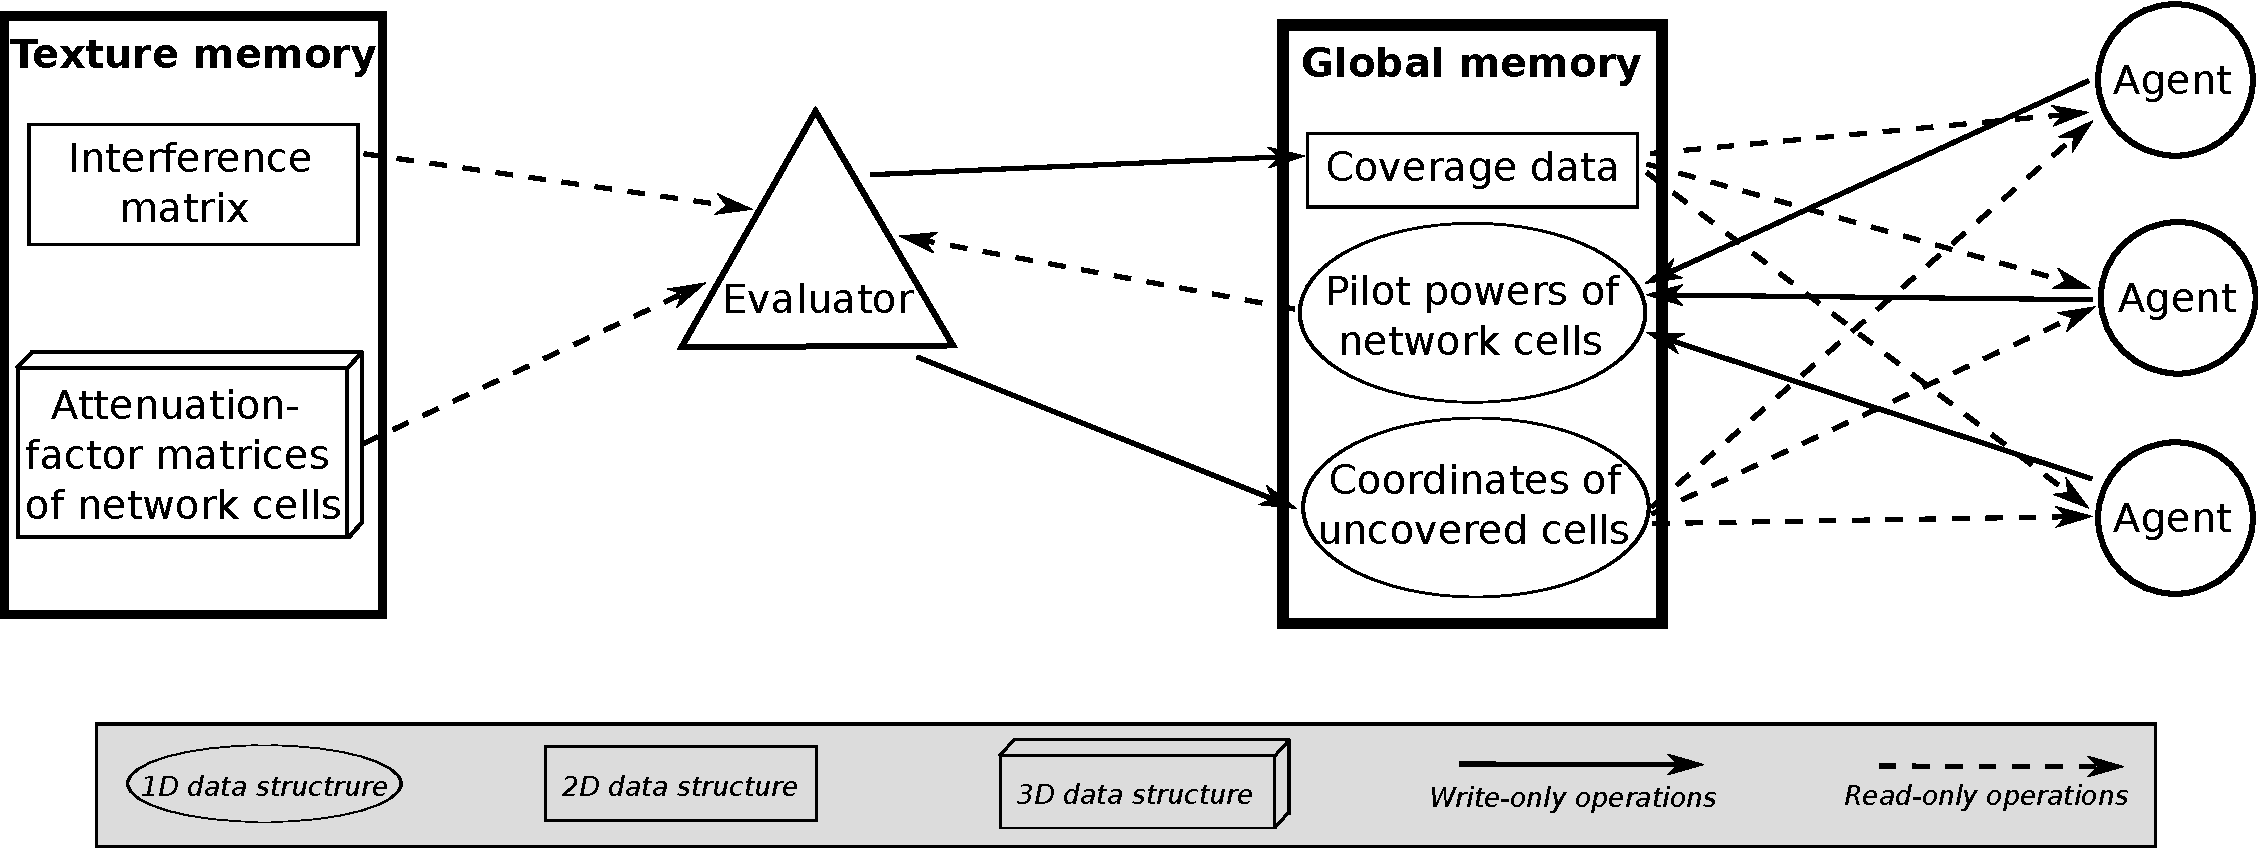
\includegraphics[width=1\textwidth]{06-experimental_evaluation-service_coverage/img/architecture}

\caption{Architecture of the parallel, agent-based optimization system on GPU.\emph{\label{fig:06-Architecture_of_the_system_on_GPU}}}
\end{figure}



\subsubsection{Objective-function evaluation}

The evaluator represents a central component of the optimization system.
It reacts to the pilot-power changes by recalculating the objective-function
value. Recall that the objective-function evaluation involves the
radio-coverage prediction of the service area and the calculation
of the total pilot power used by the cells in the target network.

After a short initialization, during which the attenuation-factor
matrices of all the cells and the interference matrix are calculated,
the evaluator computes the coverage of the service area based on the
pilot powers supplied as the initial solution. Initial solutions are
randomly generated from valid pilot-power settings that conform to
the full coverage constraint.

The evaluator also maintains a special part of the memory (see ``Coordinates
of uncovered cells'' in Figure~\ref{fig:06-Architecture_of_the_system_on_GPU})
that is intended for registering uncovered areas, i.e., $\overline{A_{\mathrm{covered}}}$.
If Equation~(\ref{eq:06-Coverage_constraint}) does not hold, the
``special'' agents randomly select a location from this portion
of memory so that a valid solution may be reached again.

It is worth mentioning that the evaluator itself has no influence
in the optimization process from a quality point-of-view. Its task
is to provide feedback and updated information to the agents that
move through the service area. From a performance point-of-view, the
importance of the evaluator is significant, as it will be shown in
the following sections.

\bigskip{}


The evaluation of the objective function was completely implemented
on the GPU using OpenCL (see Section~\ref{sub:02-OpenCL}). The reason
behind this decision is the impact objective-function evaluation has
on the performance of the optimization system as a whole, as discussed
in Section~\ref{sub:02-Black_box_optimization}. The implementation
of the agents is also based on the GPU, which drastically reduces
the number of data transfers between CPU and GPU, since all problem
elements are available on the GPU during the optimization process.
Consequently, careful memory utilization and organization are critical
to successfully accommodate all involved problem elements on the GPU,
the memory of which is significantly smaller than the RAM available
in desktop computers.


\subsubsection{Autonomous agents}

The agents apply the pilot-power changes only considering local information.
Each of them encapsulates a set of steps that is consistently applied
as it randomly moves through the service area of the network. Whenever
an agent arrives at a new location, the set of covering cells is calculated,
i.e., $C_{m}$.

The step set an agent applies following this point is directly related
to $\vert C_{m}\vert$, whereas its movement is determined by $\vert\overline{A_{\mathrm{covered}}}\vert$,
i.e., the area without service coverage.

The behavior of an agent is dictated by the pseudo-code shown in Algorithm~\ref{alg:07-Agent-behavior}.
The first four steps are responsible for guiding its movements. The
coordinates are randomly selected from two sets, $A_{\mathrm{total}}$
and $\overline{A_{\mathrm{covered}}}$. Only ``special'' agents
may move to a location without service coverage, and they apply the
step set $SS_{0}$ for as long as the solution is not valid. The portion
of ``special'' agents used for correcting a solution is a parameter
of the optimization process. During the following steps of Algorithm~\ref{alg:07-Agent-behavior},
the agent applies step sets $SS_{0}$ and $SS_{1}$ based on the number
of cells in $C_{m}$.

\begin{algorithm}
\centering

\caption{Pseudo-code representing the behavior of an agent.\textit{\label{alg:07-Agent-behavior}}}


\begin{algorithmic}
\Repeat
	\If{$is\_special\_agent()$ $\mathbf{and}$ $\overline{A_{\mathrm{covered}}}>0$}
		\State $l \gets pick\_random\_location(\overline{A_{\mathrm{covered}}})$
	\Else
		\State $l \gets pick\_random\_location(A_{\mathrm{total}})$
	\EndIf
	\State $move(l)$
	\If{$\vert C_{m}\vert=0$}
		\State $apply(SS_{0})$
	\Else
		\If{$\vert C_{m}\vert\ge 1$}
			\State $apply(SS_{1})$
		\EndIf
	\EndIf
\Until{$stopping\_criterion()$}
\end{algorithmic}
\end{algorithm}


If the current location of the agent is not covered by any cell, i.e.,
$\vert C_{m}\vert=0$, the step set $SS_{0}$ is applied (see Algorithm~\ref{alg:07-Agent_step_set_0}).
At the beginning, the cell with the lowest path loss, $c'$, that
may cover a UE at this location, is selected. If several cells have
the same $l_{cm}^{\downarrow}$ value, one of them is randomly chosen.
Once $c'$ is uniquely identified, the agent changes its pilot power
by $inc\_rate$~dB.

\begin{algorithm}
\centering

\caption{Pseudo-code representing the step set $SS_{0}$, which is applied
by the agents in areas without service coverage.\textit{\label{alg:07-Agent_step_set_0}}}


\begin{algorithmic}
\Repeat
	\State $c'\gets cell\_with\_min\_path\_loss(m)$
	\State $p_{c'}\gets adjust\_power(c',inc\_rate)$
\Until{$p_{c'}\in P_{c'}$}
\end{algorithmic}
\end{algorithm}


\begin{algorithm}
\centering

\caption{Pseudo-code representing the step set $SS_{1}$, which is applied
by the agents in areas with service coverage.\label{alg:07-Agent_step_set_1}}


\begin{algorithmic}
\Repeat
	\State $c'\gets pick\_random\_cell(C_{m})$
	\State $p_{c'}\gets adjust\_power(c',dec\_rate)$
\Until{$p_{c'}\in P_{c'}$}
\end{algorithmic}
\end{algorithm}


The step set $SS_{1}$, the pseudo-code of which is listed in Algorithm~\ref{alg:07-Agent_step_set_1},
is applied if the location of the agent is under the coverage of one
or more cells, i.e., $\vert C_{m}\vert\ge1$. The first step randomly
selects a cell from the set $C_{m}$, followed by a decrease of the
pilot power of cell $c'$. Ideally, every pixel of the geographical
area has to be covered by exactly one network cell, although this
is just a representation of a perfect solution that is unreachable
because of irregularities in the network topology and the terrain.

In both step sets, $SS_{0}$ and $SS_{1}$, the agent makes sure that
the new pilot power setting, $p_{c'}$, is an element of $P_{c'}$.
If this is not the case, cell $c'$ is discarded and another cell
is repeatedly selected at the beginning of both step sets, until this
condition is satisfied.

The values $inc\_rate$ and $dec\_rate$ are configurable parameters
that should be set before starting the optimization process. They
indicate the relative adjustment (expressed in dB) of the pilot power
of cell $c'$. On the one hand, lowering the pilot power of a cell
decreases the interference it creates within its coverage area and
those of their neighbors. Since the $\mathrm{SINR}(c,m)$ value increases
with lower interference, the coverage of $m$ may be achieved by a
neighbor cell with the same or lower pilot power. On the other hand,
increasing the pilot power of the cell with the minimum path loss
improves the coverage by evenly distributing the power among different
network cells. This cell is, on average, the nearest one to the location
of a UE $m$.

\bigskip{}


With the objective-function evaluation running on the GPU, a new performance
bottleneck appeared. The limitation factor in this case was the CPU-to-GPU
data transfers that occurred in each iteration of the optimization
process (see Section~\ref{sec:02-CUDA}).

The GPU kernel of the agents is launched as one thread block that
contains one thread per deployed agent. The thread block is organized
in a one-dimensional grid. The initial location of each agent is randomly
generated using the current system time as a random seed. Since OpenCL
provides no function for random-number generation, a simplified version
of Marsaglia's generator~\cite{Marsaglia_Seeds.for.random.number.generator:2003}
was implemented.

The analysis each agent does about the received signals at the current
location is saved into the shared memory of the thread block. It contains
the network cell and its pilot-power setting. Since both numbers are
of type \emph{short}, each of which takes up two bytes, there is enough
space in a 16~KB shared-memory block to allocate 4,096 agents. The
last step involves saving the new pilot powers into global memory.
This step is performed by only one of the threads within the thread
block in order to avoid memory-access conflicts. Updated pilot powers
are saved in negative form to indicate that coverage re-calculation
is needed for these cells. In case there are several updated pilot
powers for one network cell, the median is calculated and applied
as the new pilot power.

Even though coalesced access is not achieved by the GPU kernel of
the agents, its sole implementation provided enhanced performance.
This performance gain appears because of the lower number of data
transfers between the CPU and the GPU, since most data are available
in global memory. Moreover, the GPU kernel also produces the truly
parallel behavior of the agents, as they all apply the pilot-power
changes at the same time.


\section{Simulations \label{sec:06-Simulations}}


\subsection{Test networks}

The test networks, Net$_{1}$, Net$_{2}$ and Net$_{3}$, are subsets
of the real radio network deployed by Telekom Slovenije, d.d. The
path-loss predictions were calculated using the radio-propagation
model presented in Section~\ref{sub:04-Radio_propagation_model}.
A DEM with a 25~m$^{2}$ resolution was used as the terrain-profile
data. The requirements for the coverage threshold, $\gamma^{\mathrm{cov}}$,
were provided by experts of the Radio Network department of Telekom
Slovenije, d.d.

Net$_{1}$ is deployed over a densely populated urban area. For this
reason, the value of $\gamma^{\mathrm{cov}}$ is lower here, since
network capacity is the dominating factor, whereas coverage is flexible
because of a larger cell density, i.e., more BSs per surface unit.
Net$_{2}$ represents a network deployed over a rural area, meaning
that the network capacity can be reduced at the cost of a better coverage,
since the user density is lower. The last network, Net$_{3}$, represents
a suburban area with a densely populated, but relatively small, downtown
center, where a compromise between the network capacity and the coverage
has to be achieved.

The second group of test networks, including Net$_{4}$, Net$_{5}$
and Net$_{6}$, is part of the publicly available MOMENTUM project~\cite{Momentum.project}.
Test network Net$_{4}$ represents the city of Berlin (Germany), Net$_{5}$
represents the city of The Hague (Netherlands), and Net$_{6}$ is
the largest network optimized in~\cite{Siomina:Minimum.pilot.power.for.service.coverage},
representing a reduced version of Net$_{4}$. All networks include
information about BS locations, path-loss predictions and realistic
antennas, which are part of the scenarios provided by the MOMENTUM
project.

Network configurations that represent what could be an initial-network
setup by common-planning standards~\cite{WCDMAforUMTS_RadioAccessForThirdGenerationMobileCommunications}
were produced using the attenuation-based approach. Such configurations
can be easily calculated by a network planner. Table~\ref{tab:06-Test_network_sizes}
lists the number of BSs and cells per test network, as well as the
size of the geographical area. Different network-parameter values
used during the simulations are shown in Table \ref{tab:06-Test_network_parameters}.

\begin{table}
\caption{Sizes of the test networks used for experimentation of the service-coverage
problem, in terms of equipment and geographical area.\emph{\label{tab:06-Test_network_sizes}}}


\centering

{\small{}}%
\begin{tabular}{ccccc}
\cmidrule{2-5} 
 & {\small{Number of base stations}} & {\small{Number of cells}} & {\small{Surface {[}km$^{2}${]}}} & {\small{Resolution {[}m$^{2}${]}}}\tabularnewline\addlinespace
\midrule
{\small{Net$_{1}$}} & {\small{26}} & {\small{77}} & {\small{100.00}} & {\small{25}}\tabularnewline
{\small{Net$_{2}$}} & {\small{8}} & {\small{23}} & {\small{306.25}} & {\small{25}}\tabularnewline
{\small{Net$_{3}$}} & {\small{45}} & {\small{129}} & {\small{405.00}} & {\small{25}}\tabularnewline
{\small{Net$_{4}$}} & {\small{65}} & {\small{193}} & {\small{56.25}} & {\small{50}}\tabularnewline
{\small{Net$_{5}$}} & {\small{12}} & {\small{36}} & {\small{16.00}} & {\small{50}}\tabularnewline
{\small{Net$_{6}$}} & {\small{50}} & {\small{148}} & {\small{56.25}} & {\small{50}}\tabularnewline
\bottomrule
\end{tabular}
\end{table}


\begin{table}
\caption{Network parameters of the test networks used for the service-coverage
problem.\emph{\label{tab:06-Test_network_parameters}}}


\centering

\begin{tabular}{cccc}
\cline{2-4} 
 & $p_{c}^{k}$ & $\mathrm{N}_{0}$ & $\gamma^{\mathrm{cov}}$\tabularnewline
\hline 
Net$_{1}$ & 15.00 W & 1.55$\cdot10^{-14}$ W & 0.010\tabularnewline
Net$_{2}$ & 19.95 W & 1.55$\cdot10^{-14}$ W & 0.020\tabularnewline
Net$_{3}$ & 15.00 W & 1.55$\cdot10^{-14}$ W & 0.015\tabularnewline
Net$_{4}$ & 19.95 W & 1.55$\cdot10^{-14}$ W & 0.010\tabularnewline
Net$_{5}$ & 19.95 W & 1.55$\cdot10^{-14}$ W & 0.010\tabularnewline
Net$_{6}$ & 19.95 W & 1.55$\cdot10^{-14}$ W & 0.010\tabularnewline
\hline 
\end{tabular}
\end{table}



\subsection{Parameter settings of the parallel-agent approach \label{sub:06-Algorithm_parameter_settings}}

The parameter settings for the optimization algorithm were determined
after some experimentation with the test networks. The parameter settings
for each test networks are listed in Table~\ref{tab:06-Parameter_settings}.

\begin{table}
\caption{Parameter settings of the parallel-agent approach for each test network.\emph{\label{tab:06-Parameter_settings}}}


\centering

\begin{tabular}{ccccc}
\cmidrule{2-5} 
 & Agents & $inc\_rate$ {[}dB{]} & $dec\_rate$ {[}dB{]} & Pilot-power changes\tabularnewline\addlinespace
\midrule
Net$_{1}$ & 16 & 0.2 & -0.1 & 10,000\tabularnewline
Net$_{2}$ & 16 & 0.2 & -0.1 & 10,000\tabularnewline
Net$_{3}$ & 16 & 0.2 & -0.1 & 10,000\tabularnewline
Net$_{4}$ & 6 & 1.0 & -0.1 & 10,000\tabularnewline
Net$_{5}$ & 2 & 1.0 & -0.1 & 10,000\tabularnewline
Net$_{6}$ & 6 & 1.0 & -0.1 & 10,000\tabularnewline
\bottomrule
\end{tabular}
\end{table}


Using a higher $inc\_rate$ than $dec\_rate$ reflects the behavior
of the agents when full coverage of the service area is not guaranteed.
In practice, areas without service coverage usually appear as irregular
islands. The stopping criteria were set by limiting the total number
of pilot-power changes an agent is allowed to make. The value was
set to 10,000, even though for some of the test networks the best
solutions were found in the first quarter of the experiment.

\bigskip{}


All experiments were performed on a multi-core Intel i7 2.67~GHz
desktop computer with 6~GB of RAM running a 64-bit Linux operating
system. The GPU hardware used was an nVidia GeForce GTX~660~Ti.
The implementation language used was C, combined with OpenCL and OpenMPI
extensions.


\subsection{Results}

The results achieved by the parallel-agent approach, which are listed
in Table~\ref{tab:06-Optimization_results}, improved the optimization
objective significantly. They show that the pilot-power usage was
reduced in all networks while the service area was kept under full
coverage. Moreover, the parallel-agent solution for Net$_{1}$ improved
the attenuation-based setting by more than 300~\%. As for Net$_{2}$,
the observed improvement is around 232~\%, while the improvement
for Net$_{3}$ is more than 170~\%. 

The last test network, Net$_{6}$, is the same as N6 in~\cite{Siomina:Minimum.pilot.power.for.service.coverage}.
When comparing these results to those of~\cite{Siomina:Minimum.pilot.power.for.service.coverage},
an improvement of almost 3~\% can be observed in the solution provided
by the parallel-agent approach, i.e., 0.778 against 0.759 for the
average pilot power of Net$_{6}$.

\begin{table}
\caption{Optimization results after applying two different approaches for solving
the service-coverage problem. All values are expressed in Watts.\emph{\label{tab:06-Optimization_results}}}


\centering

\begin{tabular}{crccrc}
\cmidrule{2-6} 
 & \multicolumn{2}{c}{Attenuation-based} &  & \multicolumn{2}{c}{Parallel agents}\tabularnewline\addlinespace
\cmidrule{2-3} \cmidrule{5-6} 
 & Total power & Average pilot power &  & Total power & Average pilot power\tabularnewline\addlinespace
\cmidrule{1-3} \cmidrule{5-6} 
Net$_{1}$ & 419.292 & 5.445 &  & 137.064 & 1.780\tabularnewline
Net$_{2}$ & 78.297 & 3.404 &  & 33.344 & 1.450\tabularnewline
Net$_{3}$ & 1,014.113 & 7.861 &  & 582.954 & 4.519\tabularnewline
Net$_{4}$ & 179.876 & 0.932 &  & 145.715 & 0.755\tabularnewline
Net$_{5}$ & 73.872 & 2.052 &  & 34.884 & 0.969\tabularnewline
Net$_{6}$ & 147.014 & 0.993 &  & 112.332 & 0.759\tabularnewline
\bottomrule
\end{tabular}
\end{table}



\subsection{Performance analysis}

The graphs shown in Figures~\ref{fig:06-Convergence_Net1}, \ref{fig:06-Convergence_Net2}
and~\ref{fig:06-Convergence_Net3} depict the convergence of the
parallel-agent approach after ten independent runs for test networks
Net$_{1}$, Net$_{2}$ and Net$_{3}$, respectively. Only feasible
solutions were plotted, i.e., the solutions that meet the full-coverage
constraint. Unfeasible solutions were marked with a value of inferior
quality than the worst solution found: 428 for Net$_{1}$, 129 for
Net$_{2}$, and 1,435 for Net$_{3}$.

From the graphs of Net$_{1}$ (see Figure~\ref{fig:06-Convergence_Net1})
and Net$_{2}$ (see Figure~\ref{fig:06-Convergence_Net2}), a good
initial convergence can be observed. This is followed by a steady
improvement of the intermediate solutions. In Net$_{1}$, no additional
solution improvement is noticed towards the end of the optimization
process. This fact suggests that the stopping criteria is suitable
for this problem instance. A similar situation is observed for Net$_{2}$
that also shows a flat profile towards the end. From the graph of
Net$_{3}$ (see Figure~\ref{fig:06-Convergence_Net3}), a slower
initial convergence, followed by a steady improvement of intermediate
solutions and no significant solution enhancement towards the end,
can be observed. This convergence profile suggests that this problem
instance presents a more difficult optimization case than for Net$_{1}$
and Net$_{2}$. Indeed, this is the largest test network in terms
of surface area. However, further investigation is needed to confirm
this hypothesis. Nevertheless, the parallel-agent approach improved
the pilot-power usage of this test network by almost 75~\%.

\begin{figure}[h]
\centering

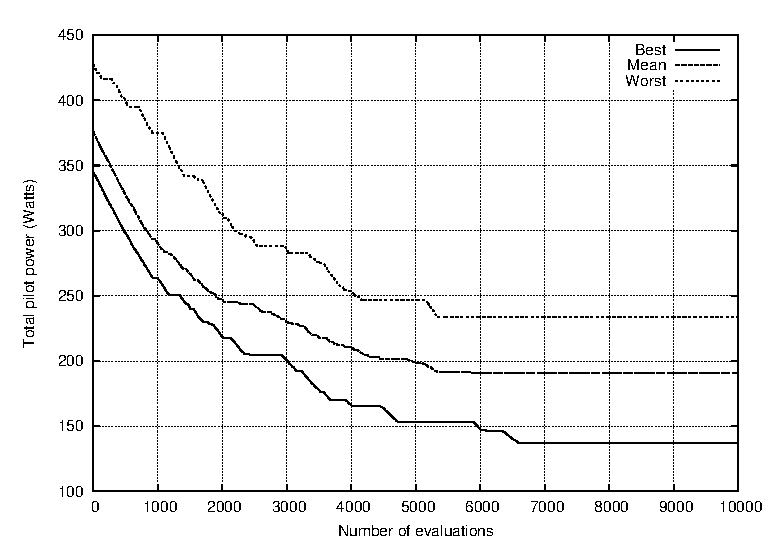
\includegraphics[width=0.7\textwidth]{06-experimental_evaluation-service_coverage/img/convergence_first}

\caption{Convergence profile of the parallel-agent approach for the test network
Net$_{1}$, deployed over an urban area.\emph{\label{fig:06-Convergence_Net1}}}
\end{figure}


\begin{figure}[h]
\centering

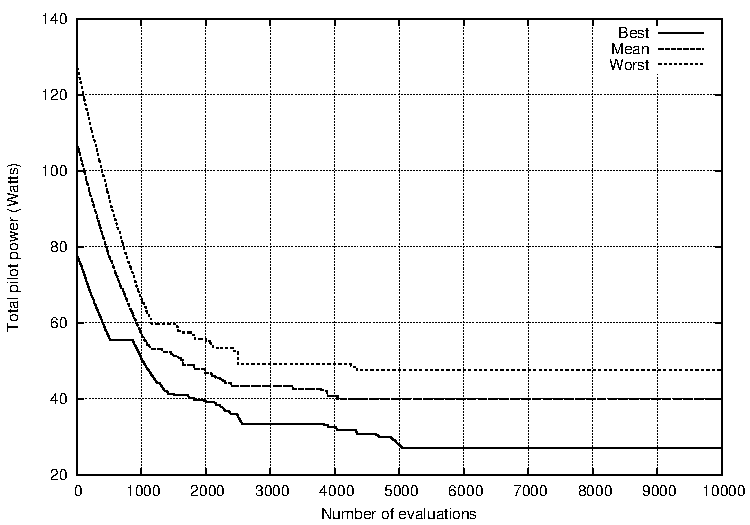
\includegraphics[width=0.7\textwidth]{06-experimental_evaluation-service_coverage/img/convergence_second}

\caption{Convergence profile of the parallel-agent approach for the test network
Net$_{2}$, deployed over a rural area.\emph{\label{fig:06-Convergence_Net2}}}
\end{figure}


\begin{figure}[h]
\centering

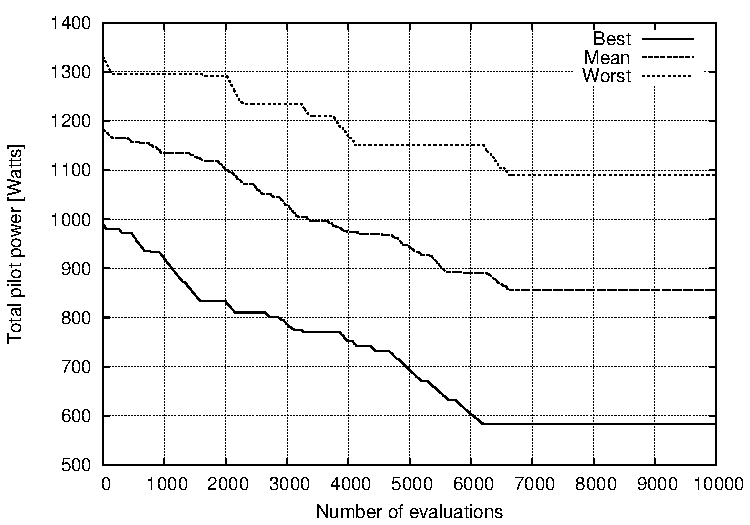
\includegraphics[width=0.7\textwidth]{06-experimental_evaluation-service_coverage/img/convergence_third}

\caption{Convergence profile of the parallel-agent approach for the test network
Net$_{3}$, deployed over a suburban area.\emph{\label{fig:06-Convergence_Net3}}}
\end{figure}


\bigskip{}


In the following, the speed-performance analysis of the experimental
simulations is presented. This analysis covers the running times during
the optimization of the first three test networks, i.e., Net$_{1}$,
Net$_{2}$ and Net$_{3}$. The running times were measured for each
implementation, and the average times, calculated after ten independent
runs, are given. The number of pilot-power changes per agent was limited
to 1,000, while all other algorithm parameters were kept at the same
values as in Section~\ref{sub:06-Algorithm_parameter_settings}.

Table~\ref{tab:06-Performance_analysis} lists the average wall-clock
times in seconds for the different implementations and test networks.
The implementations include: the CPU-MPI implementation that consists
of objective-function evaluation on CPU and parallel agents over MPI,
the GPU-MPI implementation that consists of objective-function evaluation
on GPU and parallel agents over MPI, and the GPU-GPU implementation
that consists of objective-function evaluation and parallel agents
on the same GPU. The CPU-MPI implementation is the basis for the speedup
calculation of the other two implementations.

The function evaluation on the GPU that communicates with the agents
over MPI provides the second measured setup. The evaluator implementation
takes advantage of shared memory for thread collaboration within a
thread block and texture memory for constant elements, as is it was
explained in Section~\ref{sub:04-GPU_worker_implementation}. Still,
the speedup is considerable but improvable, since numerous data transfers
between CPU and GPU are needed for the agents to access optimization-related
information. The last result set presents measurements for the complete
GPU implementation, including objective-function evaluation and agents
on the same device. The improved speedup delivered by this combination
highlights the impact that CPU-to-GPU memory transfers have on the
overall system performance. This fact is supported by the second and
third measured setups, the speedups of which exhibit, on average,
a four-fold improvement. It is also interesting to note how the speedup
gain increases with the problem-instance size. This fact confirms
that larger problem instances have a greater benefit from a parallel
implementation in terms of computational time.

\begin{table}
\caption{Wall-clock times (in seconds) and speedup factors for the different
implementations of the objective-function evaluation and the parallel
agents, as measured during the experimentation of the service-coverage
problem.\label{tab:06-Performance_analysis}}


\centering

\begin{tabular}{cccccccc}
\cmidrule{2-8} 
 & \multicolumn{1}{c}{CPU-MPI} &  & \multicolumn{2}{c}{GPU-MPI} &  & \multicolumn{2}{c}{GPU-GPU}\tabularnewline\addlinespace
\cmidrule{2-2} \cmidrule{4-5} \cmidrule{7-8} 
 & Avg. time {[}s{]} &  & Avg. time {[}s{]} & Speedup &  & Avg. time {[}s{]} & Speedup\tabularnewline\addlinespace
\cmidrule{1-2} \cmidrule{4-5} \cmidrule{7-8} 
Net$_{1}$ & 4,105 &  & 872 & 4.71 &  & 206 & 19.93\tabularnewline
Net$_{2}$ & 774 &  & 304 & 2.55 &  & 124 & 6.24\tabularnewline
Net$_{3}$ & 5,981 &  & 1,283 & 4.66 &  & 249 & 24.02\tabularnewline
\bottomrule
\end{tabular}
\end{table}



\section{Summary}

This chapter presented a novel optimization approach for solving the
well-known service-coverage problem in radio networks. The problem
addressed the full coverage of a geographical area using a minimum
amount of pilot power. The newly introduced parallel-agent approach
was successfully tested in six networks that represent real-world
scenarios. The experimental results show that the parallel-agent approach
is able to find better solutions than some heuristics, like the presented
attenuation-based approach. Moreover, the algorithm successfully tackled
larger networks, thus overcoming the obstacles of other state-of-the-art
optimization methods regarding problem-instance size~\cite{Siomina_Pilot.power.optimization:2004,Siomina:Minimum.pilot.power.for.service.coverage}.

Compared to a different optimization approach in the literature~\cite{Siomina:Minimum.pilot.power.for.service.coverage},
the solution-quality of the parallel-agent approach showed a quality
improvement. The proposed solutions, calculated for the same problem
instance as in~\cite{Siomina:Minimum.pilot.power.for.service.coverage},
were improved at the cost of a longer running time. It is worth mentioning
that it is feasible for the optimization algorithm to take a longer
time to reach the solution, since design problems, as the service-coverage
one, are usually solved offline. A comparison and analysis of the
performance of the radio-coverage prediction for real-world, radio-network
planning is later provided in Chapter~\ref{chap:08-Real-world_network_planning}.

Different implementations of the parallel-agent approach, combining
a serial version on CPU, parallel processes over MPI and GPU kernels,
were presented. In particular, GPU architectures enable the implementation
of parallel heuristics in a natural way while substantially improving
the computational-time performance. To the best of the author's knowledge,
the parallel-agent approach as presented in this chapter, has not
yet been described in the related literature.


\cleardoublepage{}


\chapter{The soft-handover balancing problem \label{chap:07-Experimental-evaluation-the-SHO-alignment-problem}}

% First paragraph has no indentation.

\noindent In Chapter~\ref{chap:06-Experimental-evaluation-the-service-coverage-problem},
an application exploiting the advantages of faster evaluation methods
has been presented. Solving the service-coverage problem for real-world
networks capitalizes on the ability to tackle bigger problem instances.
Because of their size, such problems were previously unsolvable in
a feasible amount of time. This improved performance also allows solving
optimization problems with a higher degree of complexity, usually
represented by the evaluation of multi-dimensional, non-convex objective
functions.

\noindent This chapter focuses on solving a new optimization problem
for 3G networks, that deals with downlink and uplink SHO areas (see
Section~\ref{sub:02-Handover-and-soft-handover}, Chapter~\ref{chap:02-Principles_of_mobile_radio_networks}).
By introducing a penalty-based objective function and some hard constraints,
the formal definition of the SHO-balancing problem in UMTS networks
is given. The state-of-the-art mathematical model used and the penalty
scores of the objective function are set according to the configuration
and layout of a real mobile network, deployed in Slovenia by Telekom
Slovenije, d.d. The balancing problem is then tackled by three optimization
algorithms, each of them belonging to a different category of metaheuristics.

To the best of the author's knowledge, there is no reference in the
literature of a simulation-based approach to find active downlink
and uplink SHO areas. Additionally, there are no formal optimization
methods known to the author that tackle the SHO balancing problem
as described here. The approach described in this chapter extends
the research work published by the author in \cite{Benedicic_Balancing_downlink_uplink_soft_handover_areas_in_UMTS_networks:2012}.

The remainder of this chapter is organized as follows. Section~\ref{sec:07-Motivation}
decribes the motivation behind the SHO-balancing problem, whereas
Section~\ref{sec:07-Related-work} gives an overview of other works
related to pilot-power and SHO optimization in UMTS. The static network
model is presented in Section~\ref{sec:07-Radio_network_model},
where all the elements of the mathematical model and the objective
function are defined. In Section~\ref{sec:07-Problem_definition},
the problem is formally defined, followed by a short description of
the optimization algorithms used in Section~\ref{sec:07-Optimization_algorithms}.
The simulations, including their environment and parameter setup,
are introduced in Section~\ref{sec:07-Simulations}, before their
result analysis in Section~\ref{sub:07-Results}.

\clearpage{}


\section{Motivation \label{sec:07-Motivation}}

\begin{figure}
\centering

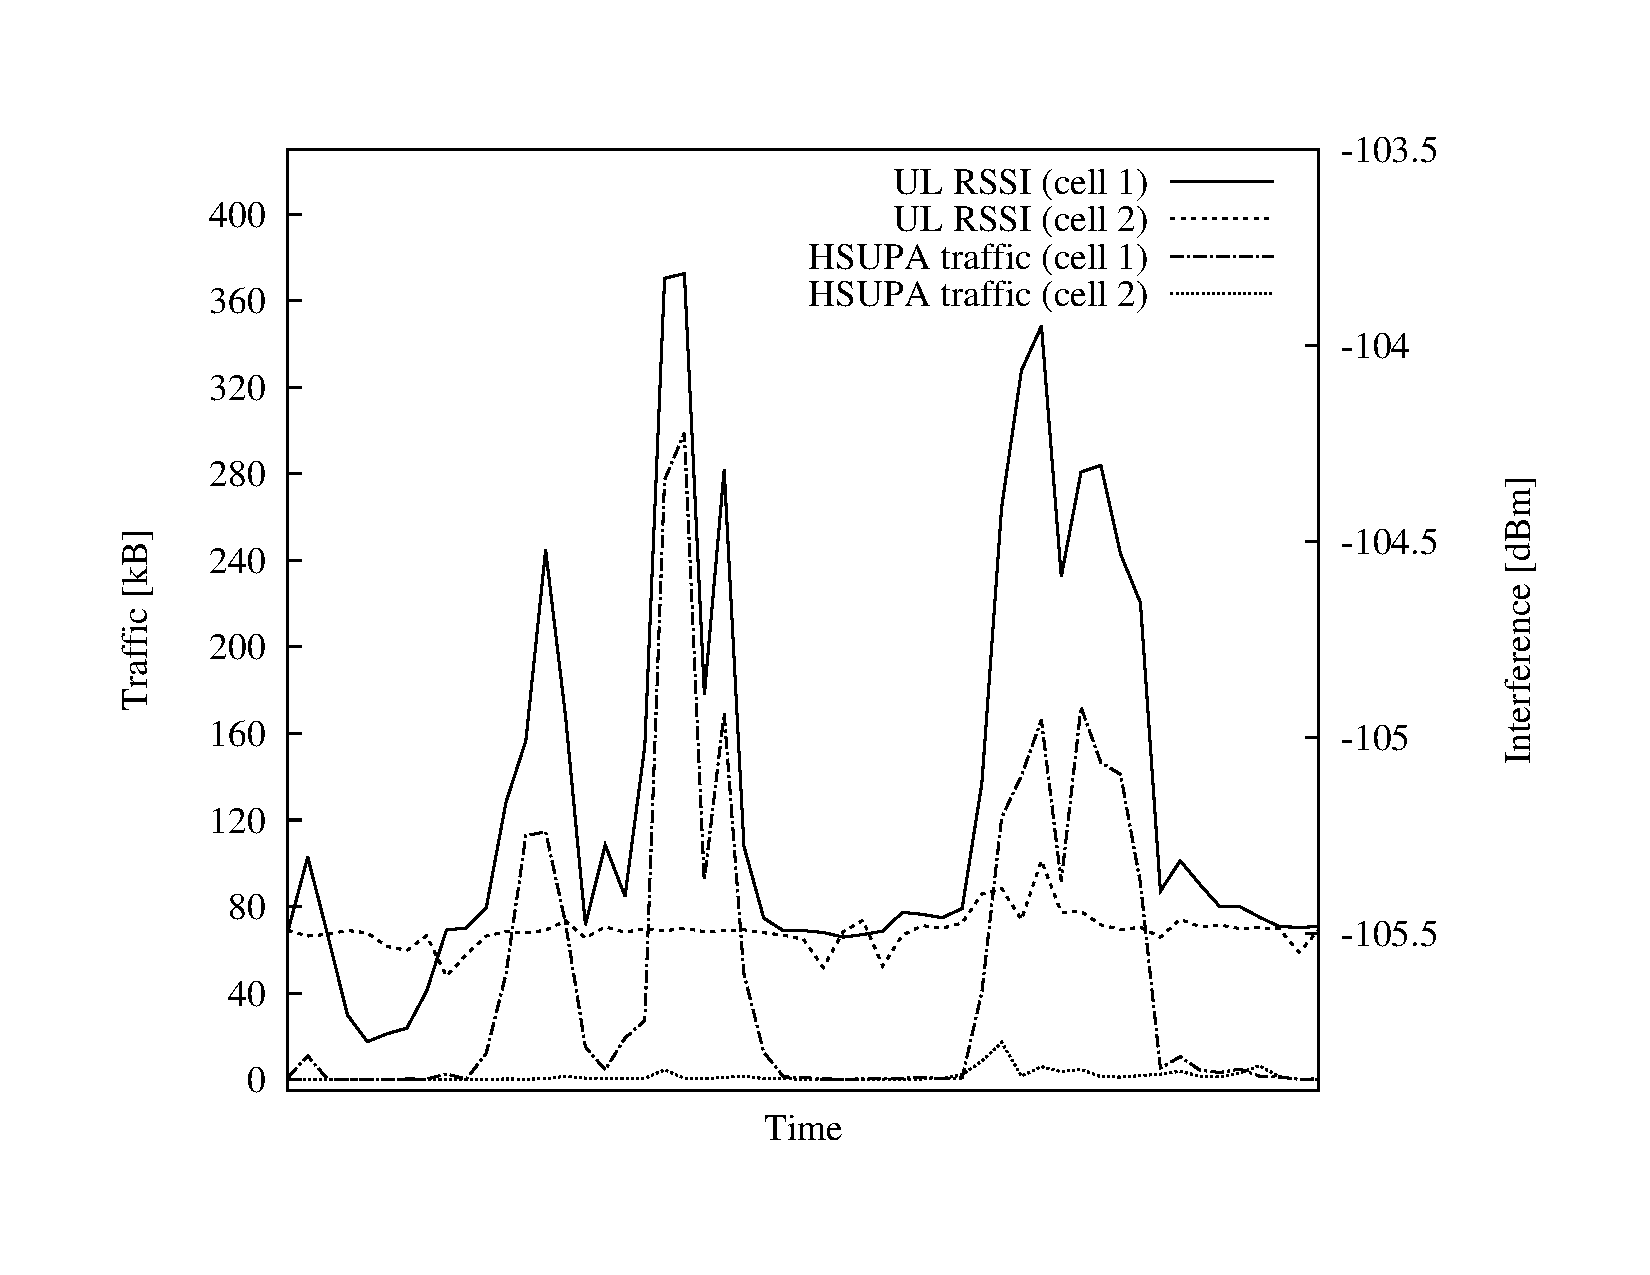
\includegraphics[width=0.9\textwidth]{07-experimental_evaluation-sho_balancing/img/network_normal}\\\vskip -0.3in(a)

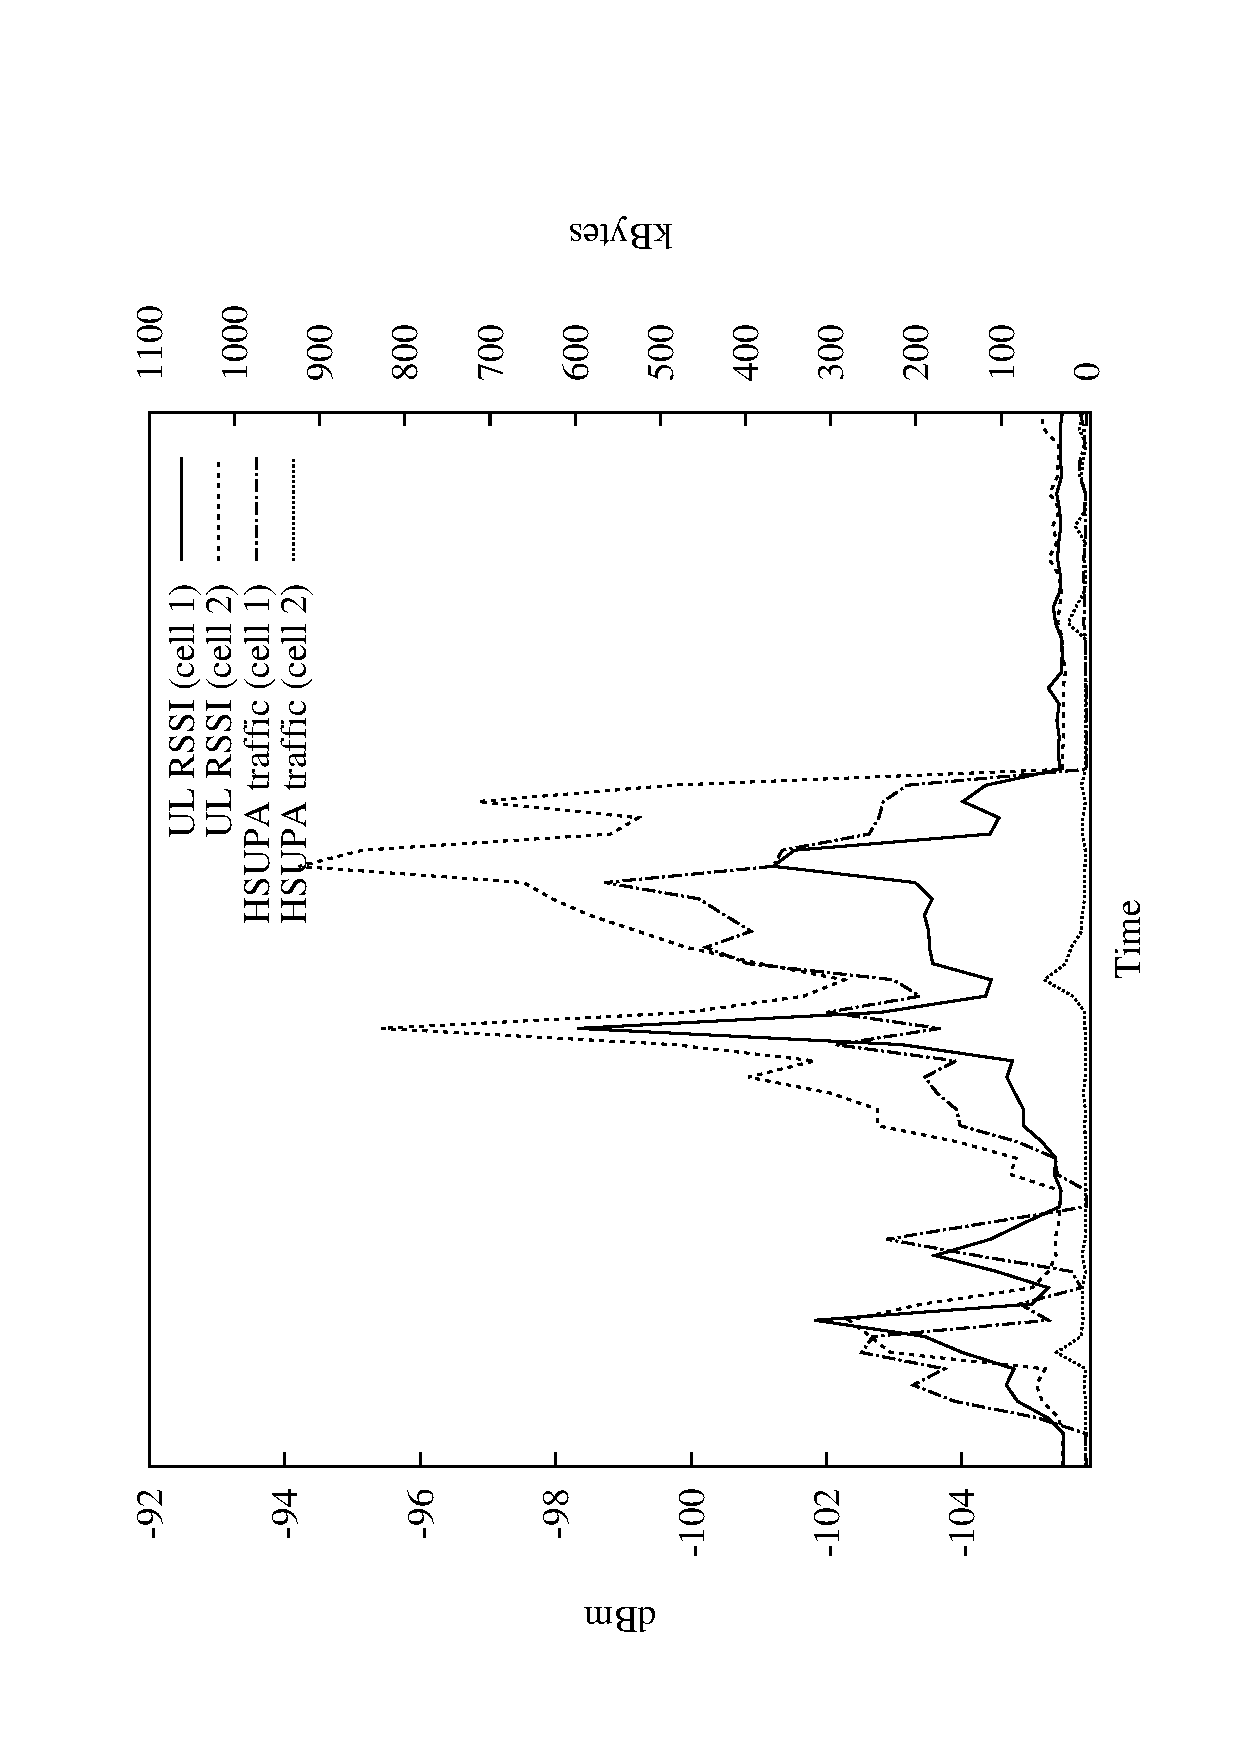
\includegraphics[width=0.9\textwidth]{07-experimental_evaluation-sho_balancing/img/network_problem}\\\vskip -0.3in(b)

\caption{HSUPA traffic and uplink interference with: (a) balanced downlink
and uplink SHO conditions, and (b) unbalanced downlink and uplink
SHO conditions.\label{fig:07-Problem_illustration}}
\end{figure}


Despite several built-in mechanisms, that allow a radio network to
overcome different problems due to the lack of SHO during a HSDPA
connection, some abnormal cases do arise, especially in those areas
where there is SHO capability in the uplink, but none in the downlink.
An example of such a case is depicted in Figure \ref{fig:07-Problem_illustration},
which shows the interference behavior during a HSPA connection in:
(a) normal SHO conditions, and (b) unbalanced SHO conditions. The
plotted data are actual radio network statistics, taken from the mobile
network deployed in Slovenia by Telekom Slovenije, d.d. The graph
on the left, (a), shows a normal HSUPA-enabled service situation,
in which the measured interference is proportional to the traffic
being served. Note how the noise rises with the increased traffic
on cell~1, while its neighbor (cell~2) has almost no interference
nor traffic. Moreover, the graph profile for both traffic and noise
of cell~1 are almost identical. The graph on the right, (b), depicts
a problematic situation, where the noise level does not only rise
on the cell serving the HSUPA services (cell~1), but also on the
neighboring one. Notice how the interference level rises on the cell
that has almost no traffic (cell~2). It is clear that the source
of this noise rise is generated by the active connection on cell~1,
which shows an increase in HSUPA traffic. However, the noise-level
profile on cell~2 does not follow its traffic, as it did in the normal
situation (a). This is due to cell~2 not being part of the active
set. Such situations appear when the UL coverage is larger than the
DL coverage. Interestingly enough, this seems to be an exceptional
case, as Holma and Toskala write in~\cite{holma2006hsdpa}, when
describing the SHO in chapter 5:

''... There is no obvious reason why the serving E-DCH cell would
not be the same as the serving HSDPA cell, and this is also required
to be the case in the specifications.''

Given the described context, the challenge is to achieve the correct
balance or distribution of downlink and uplink SHO areas within a
working UMTS network. Therefore, the network has to be fine-tuned
to improve the SHO-area balancing, thus to avoid the exceptional appearance
of problematic situations, as shown in Figure~\ref{fig:07-Problem_illustration}.
This clearly implies that the mobile network configuration should
not be excessively altered, since other aspects of the network are
working well before starting the optimization process. Hence, the
objective of the optimization problem is to find a pilot-power configuration
for all the cells in the target network, such that the balance of
downlink and uplink SHO areas is improved and other network aspects
are preserved. The optimization process takes into account different
kinds of hardware, e.g., amplifiers, cables, and antennas, adjusting
the pilot powers of the cells.

\bigskip{}


PRATO, as defined in Chapter~\ref{chap:04-Framework-design-and-implementation},
is used as the evaluation framework of the SHO-balancing problem.
A state-of-the-art mathematical model~\cite{nawrocki2006understanding}
describes the downlink and uplink SHO areas. By introducing a penalty-based
objective function and some hard constraints, a formal definition
of the SHO-balancing problem in UMTS networks is given. The mathematical
model and the penalty scores of the objective function are set according
to the configuration and layout of a real mobile network, deployed
in Slovenia by Telekom Slovenije, d.d. The SHO settings are also taken
from the actual network configuration, still they were adapted to
closely model interference and other dynamic aspects of the network.




\section{Related work \label{sec:07-Related-work}}

The SHO optimization has received quite some attention from the scientific
community during the past years. This mainly relates to the importance
it has within the deployed networks that provide high-speed services,
such as video telephony~\cite{chen2010_impact_of_soft_handover}
and data services by means of HSPA \cite{chen2011_coverage_planning_for_optimizing_HSDPA,chen2008cpich}.

Some authors tackled optimization problems at the planning stage of
the network~\cite{Eisenblatter_OptimizationMethodsForUMTSRadioNetworkPlanning,ghosh2011_optimising_CDMA_cell_planning},
considering, among other variables, BS locations and hardware. However,
most mobile operators are unable to apply such methods to a live network,
since the planning phase of the new installation has long been concluded.
Moreover, the great majority of the BSs has already been deployed
and their hardware also installed. Therefore, from the mobile operator's
point of view, mainly parameter and software optimization are the
only tools available, when it comes to QoS improvement (see Chapter~\ref{chap:02-Optimization_of_radio_networks})
and network troubleshooting in the short term.

Optimizing SHO by means of pilot-power adjustment is an established
way of enhancing network capacity, when high-speed services like HSDPA
and HSUPA coexist with legacy technologies~\cite{chen2008cpich}.
In the UMTS, the pilot power is typically between 5\% to 10\% of the
total downlink transmit power of the BS~\cite{RadioNetworkPlanningAndOptimisationForUMTS},
but there is no standardized method to fi{}nd a pilot-power setting.
A number of existing approaches to resolve this issue exist in the
related literature~\cite{WCDMAforUMTS_RadioAccessForThirdGenerationMobileCommunications,Siomina_PilotPowerManagementInWCDMANetworksCoverageControlWithRespectToTrafficDistribution,Ying_CPICHPowerSettingsInIrregularWCDMAMacroCellularNetworks},
being those based on optimization methods the most eff{}ective ones~\cite{Eisenblatter_OptimizationMethodsForUMTSRadioNetworkPlanning,GarciaLozano_CPICHPowerOptimisationByMeansOfSimulatedAnnealingInAnUTRAFDDEnvironment,RadioNetworkPlanningAndOptimisationForUMTS,UMTSRadioNetworkPlanning_OptimizationAndQoSManagementForPracticalEngineeringTasks,siomina2008minimum}.
Such a wide spectrum of available procedures is directly related to
the diverse criteria taken into account when assigning the pilot power
of a cell. The fundamental reason behind this fact is that the pilot
power is a common adjustment vairble of various optimization problems
in radio networks. This is especially true for UMTS networks, due
to their frequency-reuse factor of 1~\cite{WCDMAforUMTS_RadioAccessForThirdGenerationMobileCommunications}.


\section{Radio-network model \label{sec:07-Radio_network_model}}

This section extends the representation of the radio-network model,
previously introduced in Section~\ref{sec:06-Radio_network_model},
Chapter~\ref{chap:06-Experimental-evaluation-the-service-coverage-problem},
in order to include the SHO functionality. In this context, the mathematical
model links the SHO settings with the pilot-power level of each cell,
the best-server pattern, and the network coverage.

By introducing a change step of 0.01~dB and bounding the pilot power
of a cell $c$, $c\in C$, to $\pm2$~dB (relative to the pilot-power
setting the cell had before optimization), the number of elements
in the set $P_{c}$ is reduced. The purpose of this reduction is twofold.
First, since the optimization targets a live network, there is no
need for the algorithms to create complete new configurations, but
just to fine-tune existing ones. Second, the problem complexity is
lowered, because the size of the search space is smaller and discrete.


\subsection{Soft-handover areas \label{sub:07-SHO_areas}}

To obtain a realistic outline of the areas where an UE may potentially
maintain connections to more than one cell, a static version of the
active set, as defined in \cite{nawrocki2006understanding}, is used.
To this end, a SHO window, $\gamma^{\mathrm{sho}}$\nomenclature[S]{$\gamma^{\mathrm{sho}}$}{SHO window.},
and a \textit{\emph{maximum}} active-set size, $as^{\mathrm{max}}$\nomenclature[S]{$as^{\mathrm{max}}$}{Maximum number of neighbouring cells in the active set.},
are introduced. Both parameters are taken from the working configuration
of the real network. It follows that the cells to which an UE $m$,
$m\in M$, may maintain concurrent downlink connections are part of
the set:

\begin{eqnarray}
SHO_{m}^{\downarrow} & = & \left\{ c\vert L_{c^{*}m}^{\downarrow}p_{c^{*}}-L_{cm}^{\downarrow}p_{c}\le\gamma^{\mathrm{sho}}\right\} ,\label{eq:sho_dl}\\
\vert SHO_{m}^{\downarrow}\vert & \le & as^{\mathrm{max}},\nonumber 
\end{eqnarray}


\nomenclature[S]{$SHO_{m}^{\downarrow}$}{Cell set to which a mobile may maintain concurrent downlink connections, i.e. downlink SHO.}

\noindent where $L_{c^{*}m}^{\downarrow}$ is the downlink attenuation
factor of the best-serving cell, and $p_{c^{*}}$ is its pilot power.
Since the number of elements in $SHO_{m}^{\downarrow}$ is at most
$as^{\mathrm{max}}$, the weakest links are removed if there are several
present. This method is well suited for configurations with no hysteresis,
since dynamic effects are ignored in static models \cite{nawrocki2006understanding}. 

Additionally, in the uplink, the set of cells to which an UE can potentially
be in SHO is defined as:

\begin{equation}
SHO_{m}^{\uparrow}=\left\{ c\vert L_{mc}^{\uparrow}p_{m}^{\uparrow}\ge3.16227766\cdot10^{-12}mW\right\} ,
\end{equation}


\nomenclature[S]{$SHO_{m}^{\uparrow}$}{Cell set to which a mobile may maintain concurrent uplink connections, i.e. uplink SHO.}

\noindent where $L_{mc}^{\uparrow}$ is the uplink attenuation factor
from an UE $m$ to a cell $c$, and $p_{m}^{\uparrow}$\nomenclature[S]{$p_{m}^{\uparrow}$}{Uplink transmit power of mobile $m\in M$.}
is the uplink transmit power of $m$.

The static nature of the model intentionally neglects mobility and
dynamic interference by narrowing $\gamma^{\mathrm{sho}}$ down to
2~dB~\cite{nawrocki2006understanding}.


\section{Problem definition \label{sec:07-Problem_definition}}

Using the elements defined in Section~\ref{sec:07-Radio_network_model},
an objective function was formulated in cooperation with a team of
radio engineers of the Radio Network Department at Telekom Slovenije,
d.d. The objective function is constructed as a weighted sum, containing
different costs that penalize the occurrence of specific SHO conditions
in downlink and uplink, which may potentially cause the afore-mentioned
malfunctioning, introduced in Section \ref{sec:07-Motivation}.

A cost-based objective function is the most natural and straight-forward
way of defining the optimization objective. Besides it is easily extendable
to include other future situations, also defining the mutual importance
of the different phenomena taken into account at the optimization
phase.

Hence, the definition of the objective function for the SHO-balancing
problem is the minimization of the sum of penalty scores given as:

\begin{equation}
\min f_{\mathrm{sho}}=\sum_{c\in C}\sum_{m\in M}pf_{\mathrm{cov}}(1-cov_{cm})+pf_{\mathrm{sho}}^{\uparrow}sho_{cm}^{\uparrow}(1-sho_{cm}^{\downarrow})+pf_{\mathrm{sho}}^{\downarrow}sho_{cm}^{\downarrow}(1-sho_{cm}^{\uparrow}),\label{eq:07-objective_function}
\end{equation}


\nomenclature[S]{$f_{\mathrm{sho}}$}{Objective function of the SHO-balancing problem.}

\noindent where 

\begin{equation}
sho_{cm}^{\downarrow}=\begin{cases}
1 & c\in SHO_{m}^{\downarrow}\\
0 & otherwise
\end{cases},
\end{equation}


\begin{equation}
sho_{cm}^{\uparrow}=\begin{cases}
1 & c\in SHO_{m}^{\uparrow}\\
0 & otherwise
\end{cases},
\end{equation}


\noindent and
\begin{itemize}
\item $pf_{\mathrm{cov}}$ represents the penalty factor for uncovered areas,
\item $pf_{\mathrm{sho}}^{\uparrow}$ represents the penalty factor for
uplink SHO areas where SHO is not possible in the downlink, and
\item $pf_{\mathrm{sho}}^{\downarrow}$ represents the penalty factor for
downlink SHO areas where SHO is not possible in the uplink.
\end{itemize}
\bigskip{}


After extensive experimentation, and working in cooperation with the
radio engineers from the Radio Network Department at Telekom Slovenije,
d.d., the penalty factors from Equation~(\ref{eq:07-objective_function})
are set to the following values:
\begin{itemize}
\item $pf_{\mathrm{cov}}=15$,
\item $pf_{\mathrm{sho}}^{\uparrow}=13$, and
\item $pf_{\mathrm{sho}}^{\downarrow}=3$.
\end{itemize}
It is clear that the coverage is the most important quality aspect
from the network point of view (penalty factor $pf_{\mathrm{cov}}$).
Moreover, it imposes the biggest constraint to the optimization process,
since the balance between SHO areas should not sacrifice network coverage.
Another important characteristic that emerges from these values is
the preference for minimizing areas where SHO capability is available
in the uplink, but not in the downlink (penalty factor $pf_{\mathrm{sho}}^{\uparrow}$).
As it has been described in Section~\ref{sec:07-Motivation}, the
consequences of such SHO arrangement produce severe interference in
neighboring cells (Figure~\ref{fig:07-Problem_illustration}), which
may also result in service inaccessibility. The last factor $pf_{\mathrm{sho}}^{\downarrow}$
imposes a penalty value over areas where the SHO capability is available
in the downlink, but not in the uplink. Recall that when accessing
HSPA services, SHO is available only in the uplink. For this reason,
the link throughput may benefit from the SHO in the uplink if it is
available. The relative lower importance of the last penalty factor,
when compared to the other ones, is directly related to the consequences
of the unbalancing that such SHO areas may have on the network. In
this case, only the HSPA throughput is affected, while the service
accessibility should not be an issue, given there is enough uplink
coverage~\cite{holma2006hsdpa}.


\section{Optimization approaches \label{sec:07-Optimization_algorithms}}

The SHO-balancing problem has been tackled using three fundamentally
different optimization algorithms, namely:
\begin{itemize}
\item DE (see Section~\ref{sub:02-DE}, Chapter~\ref{chap:02-Optimization_models}),
from the family of evolutionary algorithms;
\item DASA (see Section~\ref{sub:02-DASA}, Chapter~\ref{chap:02-Optimization_models}),
from the family of swarm-intelligence algorithms; and
\item SA (see Section~\ref{sub:02-SA}, Chapter~\ref{chap:02-Optimization_models}),
from the group of classic metaheuristic algorithms, targeted at combinatorial
optimization problems.
\end{itemize}
Each of these algorithms shall minimize the objective function value
by adopting essentially disparate approaches, hence the diversity
of applying algorithms belonging to different families to solve the
same optimization problem. Therefore, the result analysis shall establish
which of the presented approaches is better suited for solving the
SHO-balancing problem.

The following sections describe how the SHO-balancing problem is represented
by the internal structure of each of the selected algorithms and their
controlling parameters.


\subsection{Differential evolution}

The DE algorithm features a parallel direct search method, which utilizes
a population of $D$-dimensional parameter vectors. The SHO-balancing
problem is expressed in each component of a vector $X$ of the population,
which represents the pilot power of a target cell, i.e.:

\begin{equation}
X_{aG}=\left\{ x_{1},x_{2},\ldots x_{c},\ldots,x_{D}\right\} ,\label{eq:07-DE_mapping}
\end{equation}
where $x_{c}\in P_{c}$ represents a candidate pilot-power setting
of cell $c$, and $G$ indicates the generation of an individual $a$
in the population. Since there are $|C|$ cells in a mobile network,
it follows that the population size, $D=|C|$.

From the different variants of DE, the most popular one is used here,
called \emph{DE/rand/1/bin}. The nomenclature used to name this variant
indicates the way the algorithm works:
\begin{itemize}
\item \emph{DE }denotes the differential evolution algorithm,
\item \emph{rand }indicates that the individuals selected to compute the
mutation values are randomly chosen,
\item 1\emph{ }specifies the number of pairs of selected solutions used
to calculate the crossover vector, and
\item \emph{bin }means that a binomial recombination operator is used.
\end{itemize}

\subsection{Differential ant-stigmergy algorithm}

The mapping between the balancing problem and DASA is similar to the
one for DE:

\begin{equation}
X_{a}=\left\{ x_{1},x_{2},\ldots x_{i},\ldots,x_{D}\right\} \label{eq:07-DASA_mapping}
\end{equation}


\noindent In this case, each ant, $a$, creates its own solution vector,
$X_{a}$, during the minimization process. At the end of every iteration,
and after all the ants have created solutions, they are evaluated
to establish if any of them is better than the best solution found
so far.


\subsection{Simulated annealing}

From the SA perspective, the system under optimization is in a given
\emph{state} at each time step during the process. The objective function
maps a system state to a value known as the \emph{energy} of the system
in that state. A \emph{move} in the search space represents a change
in the state of the system. After making a move, the system may exhibit
lower or higher energy, depending on the results of the objective
function.

Algorithm~\ref{alg:07-SA_move} shows the pseudo-code of a move in
the search space of possible pilot-power settings, resulting in a
new state of the system.

\begin{algorithm}
\centering

\caption{A move in the search space of SA for solving the SHO-balancing problem.\label{alg:07-SA_move}}


\begin{algorithmic}
\State $\mathbf{c'} \gets pick\_random\_cell(C)$
\Repeat
	\If{$ \mathrm{uniform}[0,1] < 0.5$}
		\State $p_{c'}^{\mathrm{new}} \gets p_{c'}+0.01$
	\Else
		\State $p_{c'}^{\mathrm{new}} \gets p_{c'}-0.01$
	\EndIf
\Until{$p_{c'}^{\mathrm{new}}\in P_{c'}$}
\State $p_{c'} \gets p_{c'}^{\mathrm{new}}$
\end{algorithmic}
\end{algorithm}


At the first step, a cell, $c'$, is randomly selected from the set
of all cells in the network, $C$. In step 2, a change of +0.01~dB
or -0.01~dB is applied with 50\% probability to $p_{c'}$. The pilot
power of cell $c'$ is expressed in dBm. The randomly generated pilot-power
setting, $p_{c'}^{\mathrm{new}}$, is checked for validity in step
3, i.e., it must be an element of the set $P_{c'}$. If $p_{c'}^{\mathrm{new}}$
is not a valid pilot power, step 2 is executed again, generating another
random pilot power. Finally, in step 4, the pilot power of cell $c$
is replaced by $p_{c'}^{\mathrm{new}}$.

It is important to note that, as long as $|P_{c'}|>1$, the pseudo-code
shown in Algorithm~\ref{alg:07-SA_move} shall never be trapped in
an endless loop. On the other hand, if $|P_{c'}|<2$, there are no
candidate pilot powers for cell $c'$, and thus there is no possibility
of optimization. Notice also that the acceptance of a move in the
search space is left to SA and its stochastic components.


\section{Simulations \label{sec:07-Simulations}}

The simulations were performed over the target geographical area,
for which DEM and clutter data were available. The mobile users were
assumed to be uniformly distributed. The SHO conditions were determined
by the relative received-signal quality from different cells, and
the SHO window, which triggers the addition of a cell to a user's
active set~\cite{WCDMAforUMTS_RadioAccessForThirdGenerationMobileCommunications}.


\subsection{Test network}

The test network used for the simulations, Net$_{7}$, is a subset
of the real UMTS network deployed in Slovenia by Telekom Slovenije,
d.d. It represents a network extending over a hilly terrain, combining
both rural and middle-dense suburban areas, which contains 25 cells
within an area of more than 150~km$^{2}$. Table~\ref{tab:07-Test_network_properties}
shows some characteristics of the test network used, and Figure~\ref{fig:07-Coverage_areas}
shows the area under radio coverage, $A_{\mathrm{covered}}$, within
$A_{\mathrm{total}}$.

\begin{table}[h]
\caption{Technical characteristics of Net$_{7}$, the test network used for
the SHO-balancing problem. \label{tab:07-Test_network_properties}}


\centering

\begin{tabular}{cc}
\hline 
Number of cells & $25$\tabularnewline
Coverage threshold (RSCP) & $-115$~dBm\tabularnewline
SHO window ($\gamma^{\mathrm{sho}}$) & $2$~dB\tabularnewline
User equipment ($p_{m}^{\uparrow}$) & $21$~dBm, power class 4\tabularnewline
Pixel resolution & $25$~m$^{2}$\tabularnewline
Population density & $398$/km$^{2}$\tabularnewline
\hline 
\end{tabular}
\end{table}


\begin{figure}
\centering

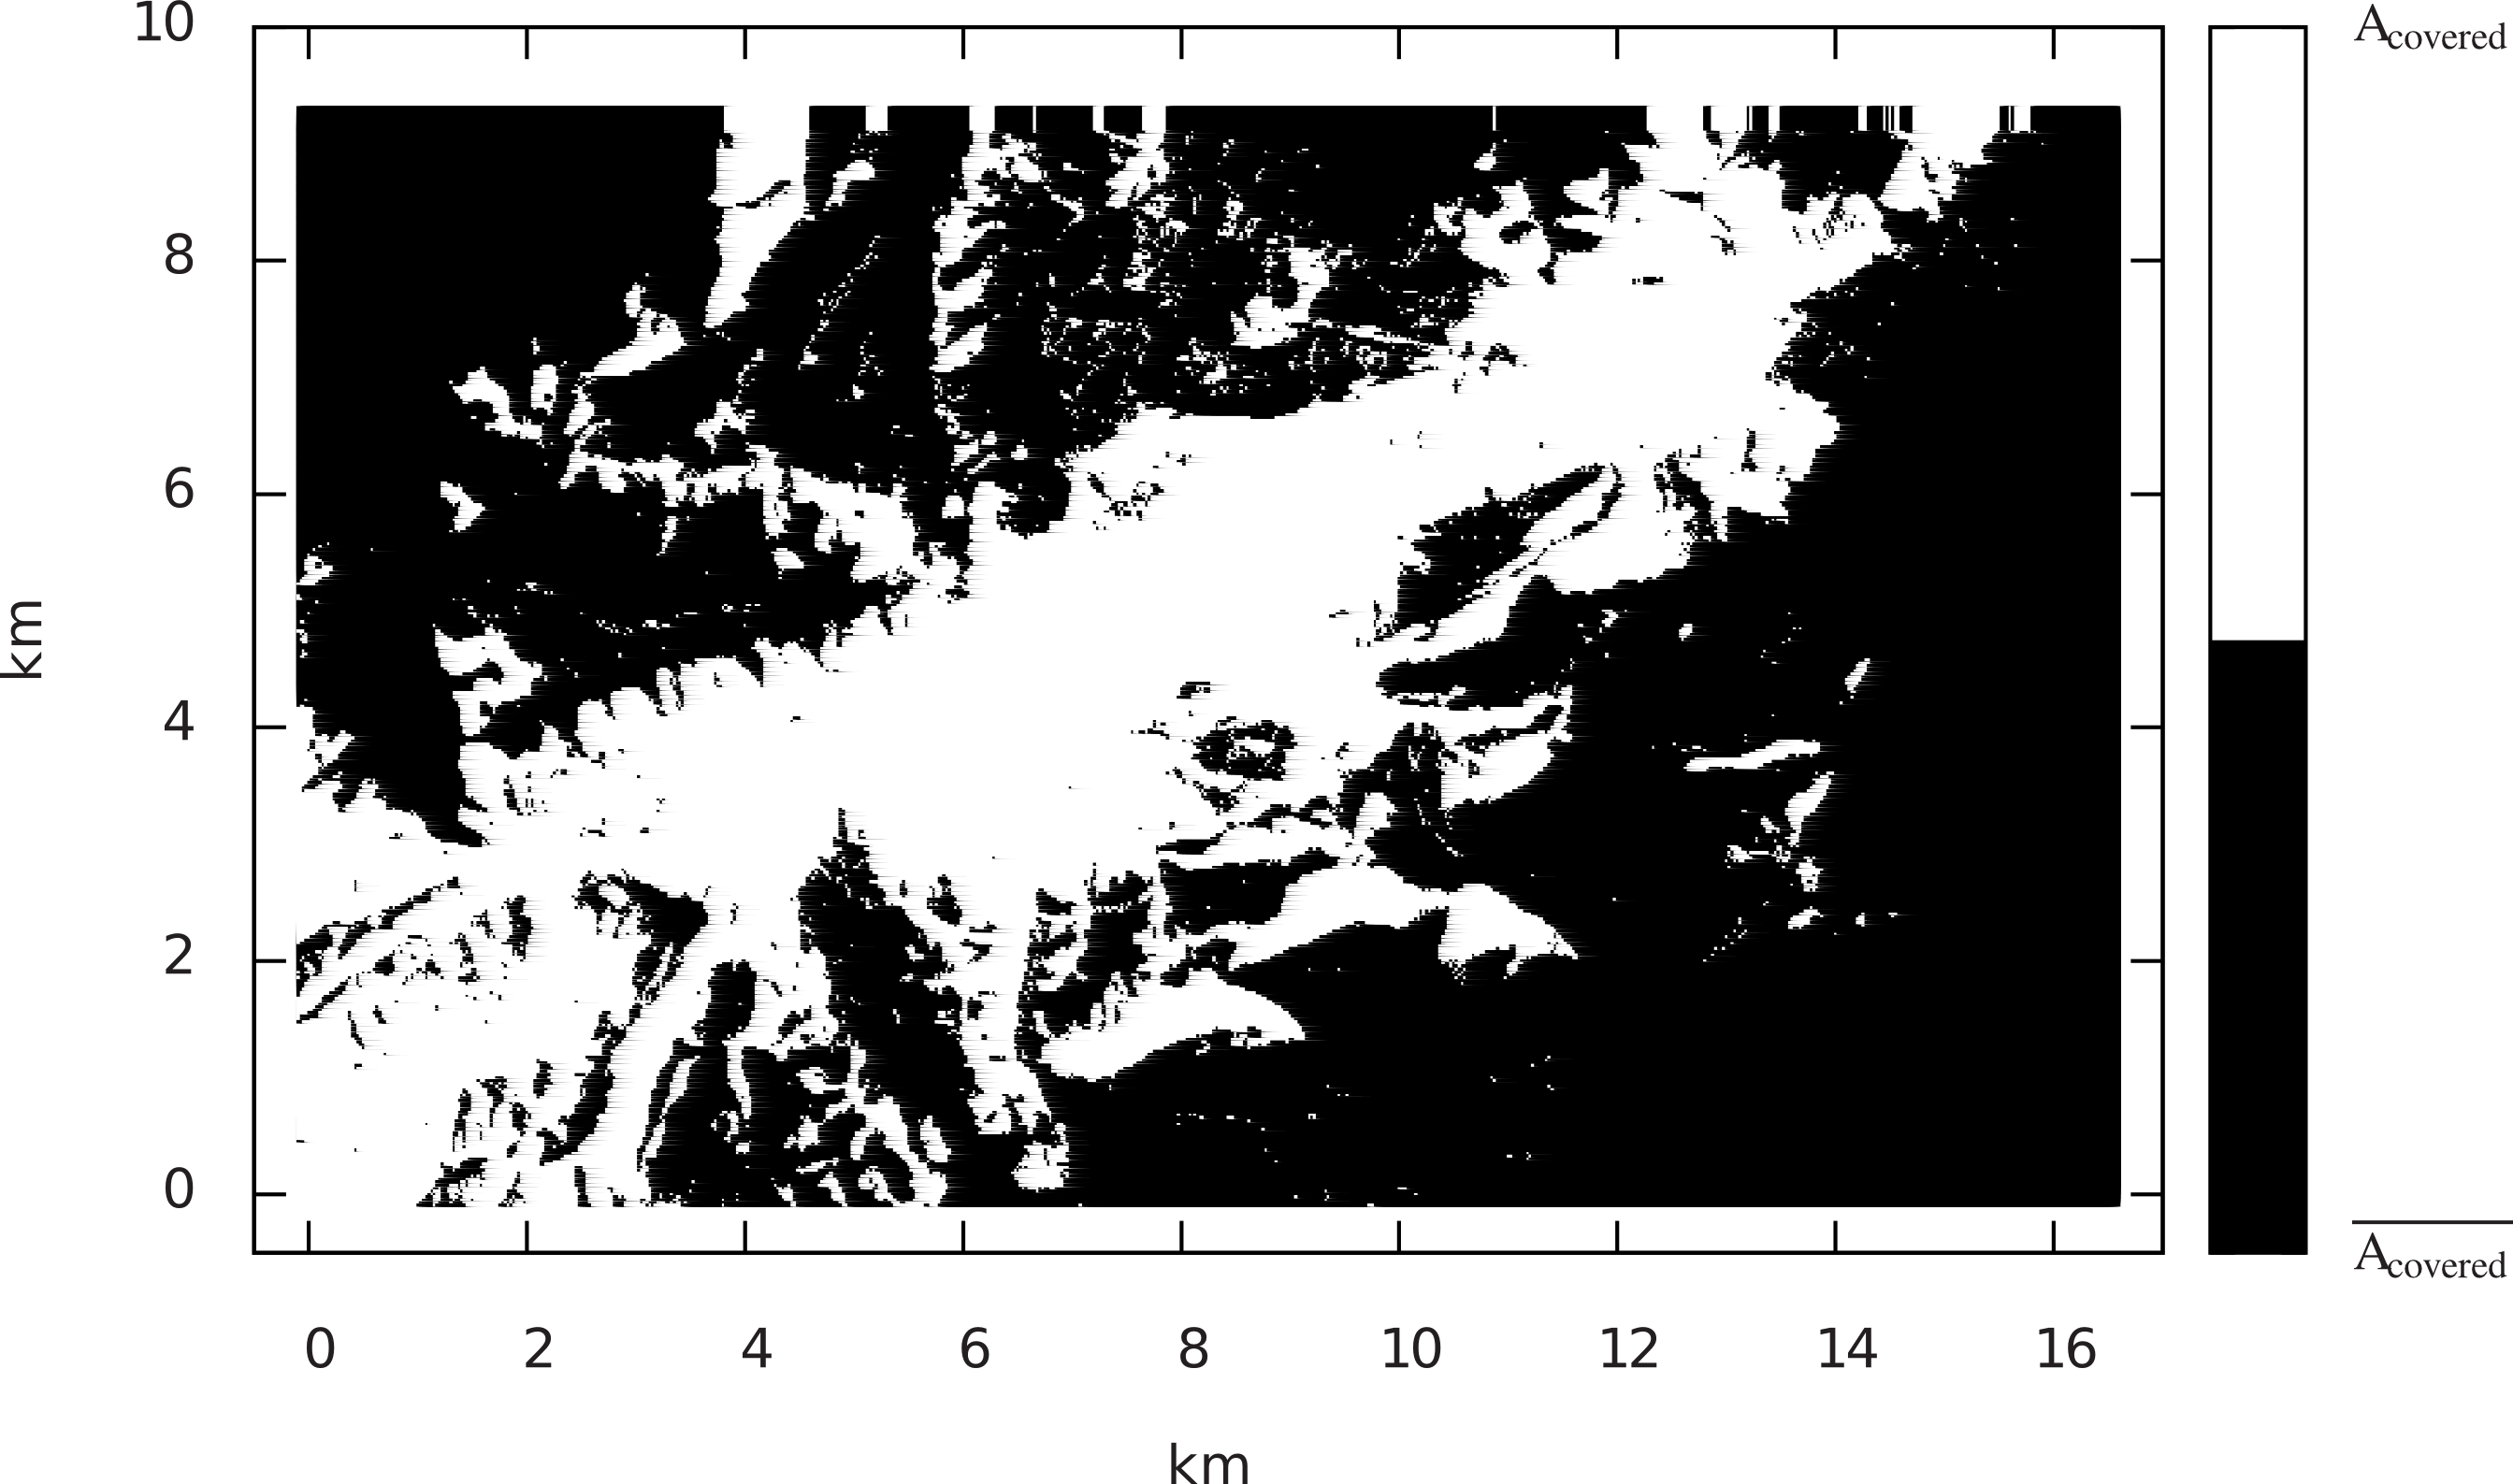
\includegraphics[width=1\textwidth]{07-experimental_evaluation-sho_balancing/img/coverage_area}

\caption{Area under radio coverage, $A_{\mathrm{covered}}$, and without radio
coverage, $\overline{A_{\mathrm{covered}}}$, within the complete
geographical area, $A_{\mathrm{total}}$, of test network Net$_{7}$.\label{fig:07-Coverage_areas}}
\end{figure}



\subsection{Algorithm parameters}

In this section, the algorithm-parameter setup used during the simulations
is given. In all three cases, the parameter names are given with their
respective values and descriptions.

The parameters controlling the behavior of the DE algorithm were set
as follows:
\begin{itemize}
\item $NP=100$, the population size;
\item $G_{max}=1000$, the maximum number of generations for the algorithm
to run;
\item $CR=0.8$, the crossover constant; and
\item $F=0.5$, the mutation-scaling factor.
\end{itemize}
As for DASA, the parameters were set to the following values:
\begin{itemize}
\item $m=10$, the number of ants;
\item $b=10,$ the discrete base;
\item $q=0.2$, the pheromone dispersion factor;
\item $s_{+}=0.01$, the global scale-increasing factor;
\item $s_{-}=0.01$, the global scale-decreasing factor; and 
\item $e=1.0^{-2}$, the maximum parameter precision.
\end{itemize}
There are only two parameters controlling SA, namely:
\begin{itemize}
\item $t_{initial}=125$, the initial temperature; and
\item $it=100,000$, the total number of iterations.
\end{itemize}
In this case, the exponential-lowering schema was chosen as the way
the temperature was lowered during the SA searches.


\subsection{Experimental environment}

All experiments were carried out on a 4-core Intel i7 2.67~GHz desktop
computer with 6~GB of RAM running a 64-bit Linux operating system.
The implementation languages used were C and Python, with the latter
mostly used as \textquoteleft{}glue\textquoteright{} to hold the different
implementation parts together, as well as for I/O operations. To lower
the time needed to run one optimization round, the entire objective-function
evaluation was implemented using OpenCL and executed on a nVidia GeForce
GTX 260. This individual change exhibited more than 15-fold, execution-time
speedup, when compared to the original CPU-only version.


\subsection{Results \label{sub:07-Results}}

In this section, the performance of the selected algorithms is presented.
The analysis includes aspects related to solution quality and convergence
speed. All experimental results were obtained after 30 independent
runs, each of them limited to a maximum of 100,000 evaluations. The
gathered results are shown in Table~\ref{tab:07-Algorithm_performance}.

\begin{table}
\centering

\caption{Solution-quality performance of the three algorithms, after 30 independent
runs\textit{\emph{.}}\textit{\label{tab:07-Algorithm_performance}}}


\begin{tabular}{ccccc}
\toprule 
 & Best & Worst & Mean & Std. deviation\tabularnewline\addlinespace
\midrule
DE & 2,286,292.00 & 2,286,541.00 & 2,286,517.09 & 62.06\tabularnewline
DASA & 2,286,446.00 & 2,286,633.00 & 2,286,592.00 & 26.19\tabularnewline
SA  & 2,293,350.00 & 2,295,570.00 & 2,294,626.50 & 663.75\tabularnewline
\bottomrule
\end{tabular}
\end{table}


It may be observed that DE reached the lowest objective-function value,
closely followed by DASA. Likewise, both algorithms arrived at very
similar results for the worst, mean and standard-deviation values.
SA, on the other hand, did not achieve comparable values, since its
results are behind those of DE and DASA. Notice that even the best
SA solution is no better than the worst solution of DASA. Moreover,
the standard deviation exhibited by SA is one order of magnitude bigger
than those of DASA and DE.

\begin{figure}
\centering

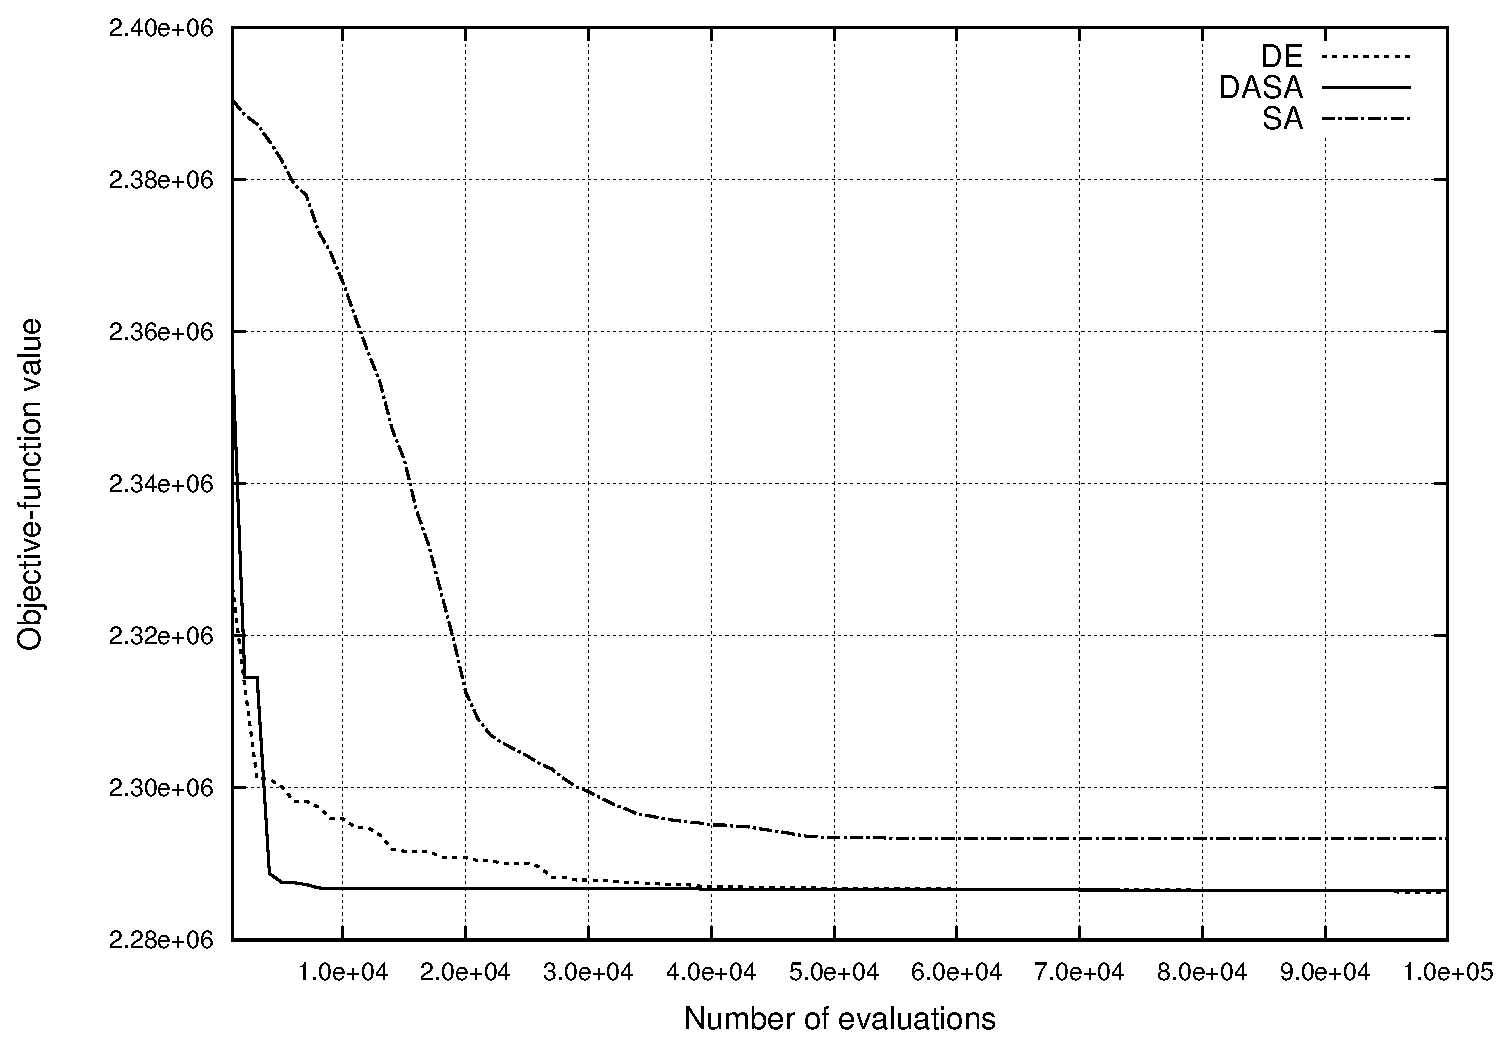
\includegraphics[width=0.9\textwidth]{07-experimental_evaluation-sho_balancing/img/algorithm_convergence}

\caption{Convergence analysis for each of the three algorithms, i.e., DE, DASA
and SA, showing the best results obtained for the SHO-balancing problem.\label{fig:07-Algorithm_convergence}}
\end{figure}


The convergence of the best-recorded run of each of the three algorithms
is shown in Figure~\ref{fig:07-Algorithm_convergence}. It is worth
mentioning that every optimization run starts from a different solution,
randomly constructed by picking a pilot-power setting, $p_{c}^{k}$,
from every $P_{c}$, $1\le k\le|P_{c}|$, $\forall c\in C$. Notice
how fast DASA converged to a good solution. After a number of evaluations
without improvement, DASA resets itself and continues searching from
a new random point within the search space \cite{korosec2010_DASA}.
DE also converged considerably fast, although not as fast as DASA
did. It this case, DE does not reset itself if the current solution
cannot be improved. Despite this, and based on the flat profile the
graph exhibits towards the end of the optimization run, it is clear
that 100,000 evaluations is an adequate stopping criterion for all
algorithms. The third algorithm, SA, slowly converged towards the
best solution found, even though it was not as good as the solutions
found by DE and DASA. 

The three convergence profiles shown in Figure~\ref{fig:07-Algorithm_convergence}
give a clearer notion about the way these algorithms explore the search
space of the SHO-balancing problem.

The simulation-running times have been intentionally omitted, since
the algorithm implementations are fundamentally different and therefore
not comparable with each other.


\subsubsection{Performance analysis}

\begin{table}
\centering

\caption{Improvement analysis of the best solution that each algorithm achieved
for the SHO-balancing problem.\textit{\label{tab:07-Optimization_result_analysis}}}


{\scriptsize{}}%
\begin{tabular}{ccccccc}
\toprule 
 & {\scriptsize{Uncovered}} & {\scriptsize{Covered, no SHO}} & {\scriptsize{SHO}} & {\scriptsize{no SHO$^{\downarrow}$, SHO$^{\uparrow}$}} & {\scriptsize{SHO$^{\downarrow}$, no SHO$^{\uparrow}$}} & {\scriptsize{Total}}\tabularnewline\addlinespace
\midrule
{\scriptsize{Before opt.}} & {\scriptsize{63.00 \%}} & {\scriptsize{15.11 \%}} & {\scriptsize{15.73 \%}} & {\scriptsize{1.80 \%}} & {\scriptsize{4.36 \%}} & {\scriptsize{100.00 \%}}\tabularnewline
\cmidrule{2-7} 
{\scriptsize{DE sol.}} & {\scriptsize{60.23 \%}} & {\scriptsize{16.13 \%}} & {\scriptsize{16.09 \%}} & {\scriptsize{1.47 \%}} & {\scriptsize{6.08 \%}} & {\scriptsize{100.00 \%}}\tabularnewline
{\scriptsize{DASA sol.}} & {\scriptsize{60.24 \%}} & {\scriptsize{16.16 \%}} & {\scriptsize{16.90 \%}} & {\scriptsize{1.46 \%}} & {\scriptsize{5.24 \%}} & {\scriptsize{100.00 \%}}\tabularnewline
{\scriptsize{SA sol.}} & {\scriptsize{60.42 \%}} & {\scriptsize{16.55 \%}} & {\scriptsize{15.97 \%}} & {\scriptsize{1.56 \%}} & {\scriptsize{5.50 \%}} & {\scriptsize{100.00 \%}}\tabularnewline
\cmidrule{2-7} 
{\scriptsize{DE impr.}} & {\scriptsize{+4.40 \%}} & {\scriptsize{+6.75 \%}} & {\scriptsize{+2.29 \%}} & {\scriptsize{+18.33 \%}} & {\scriptsize{-39.45 \%}} & {\scriptsize{---}}\tabularnewline
{\scriptsize{DASA impr.}} & {\scriptsize{+4.38 \%}} & {\scriptsize{+6.95 \%}} & {\scriptsize{+7.44 \%}} & {\scriptsize{+18.88 \%}} & {\scriptsize{-20.18 \%}} & {\scriptsize{---}}\tabularnewline
{\scriptsize{SA impr.}} & {\scriptsize{+4.09 \%}} & {\scriptsize{+9.53 \%}} & {\scriptsize{+1.52 \%}} & {\scriptsize{+13.33 \%}} & {\scriptsize{-26.15 \%}} & {\scriptsize{---}}\tabularnewline
\cmidrule{2-7} 
{\scriptsize{Avg. impr.}} & {\scriptsize{+4.29 \%}} & {\scriptsize{+7.74 \%}} & {\scriptsize{+3.75 \%}} & {\scriptsize{+16.85 \%}} & {\scriptsize{-28.59 \%}} & {\scriptsize{---}}\tabularnewline
\bottomrule
\end{tabular}
\end{table}


Table~\ref{tab:07-Optimization_result_analysis} presents the analysis
of the obtained results from the network point of view. After 30 independent
runs of each of the three algorithms, the best results obtained where
evaluated for the improvement and the decline of each of the measured
network-performance aspects. The results are shown in Table~\ref{tab:07-Optimization_result_analysis},
where '+' indicates improvement and '-' indicates a decline of a given
criteria. Overall, it may be observed that the measured criteria have
been significantly improved. The only exception is the measure for
downlink SHO, without SHO in the uplink (labeled as `SHO$^{\downarrow}$,
no SHO$^{\uparrow}$'), which shows an expected decline, since it
is the optimization aspect with the lowest penalty-factor value.

The coverage has been improved with an average of 4.29\%, whereas
the coverage area where there is no SHO capability, has been increased
7.74\% in average. Areas where SHO is available in both downlink and
uplink have also been improved, i.e., 3.75\% in average. This particular
improvement is interesting from the optimization point of view, because
it had no explicit penalty factor set. Therefore, this may be understood
as a consequence of the correct representation of the different network
aspects in the objective function.

\begin{figure}[H]
\centering

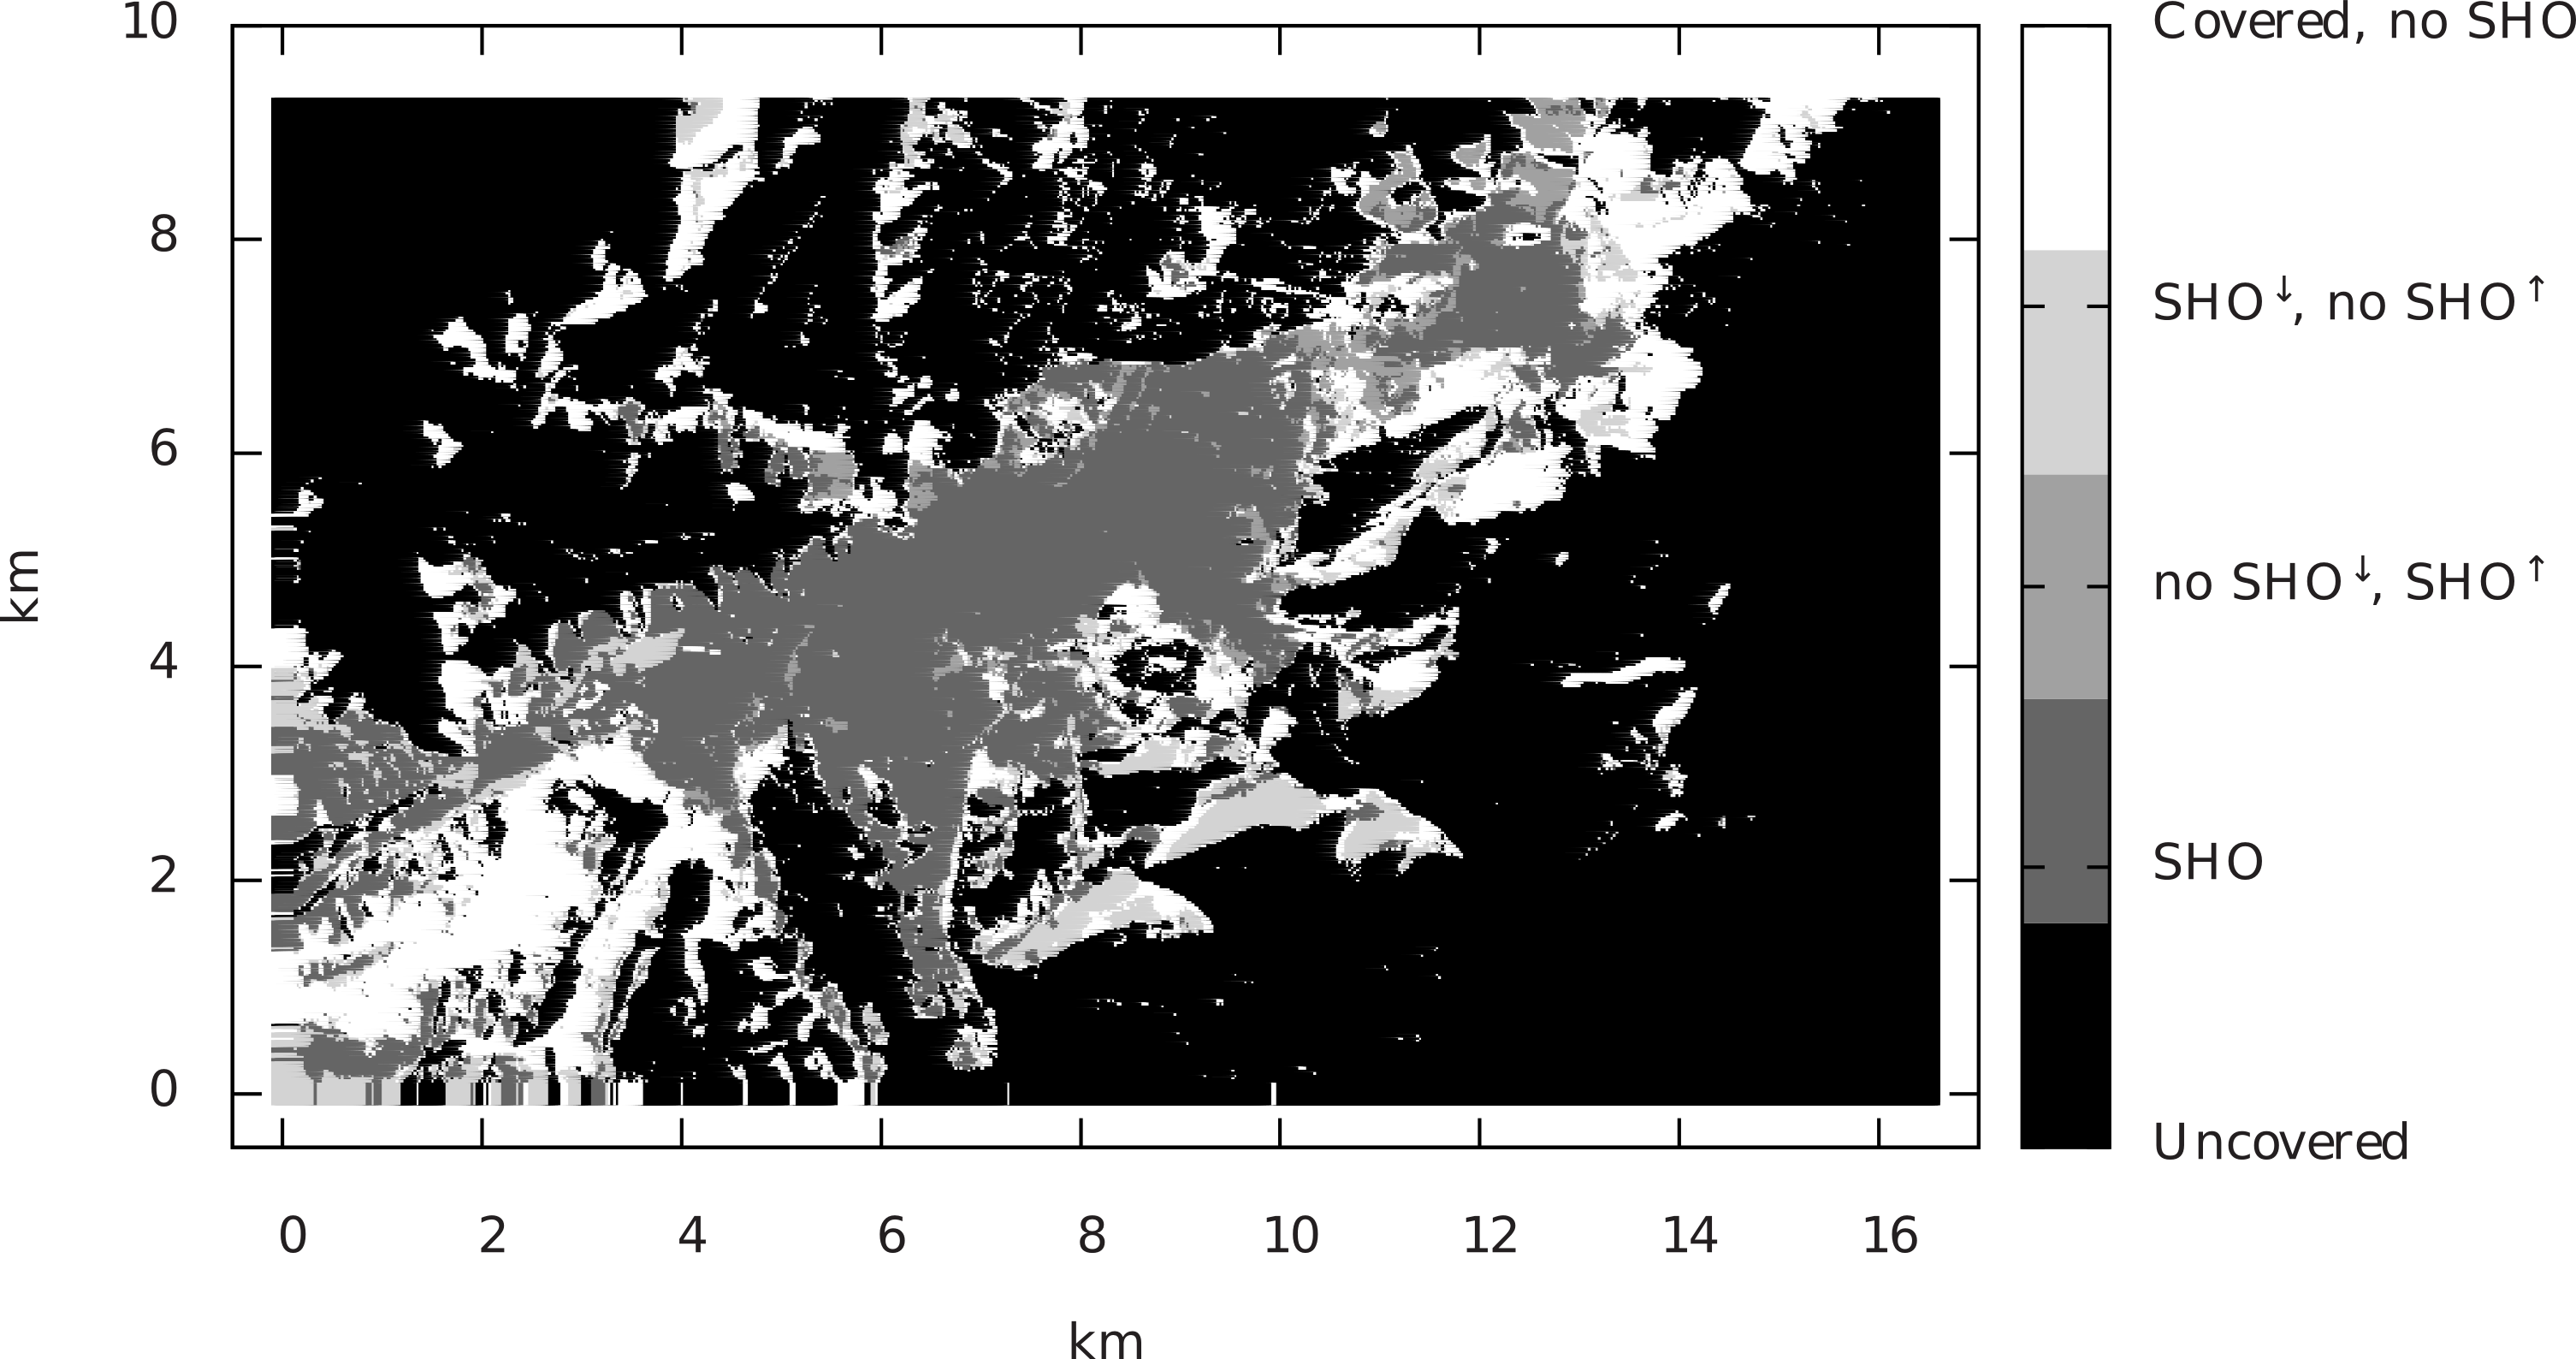
\includegraphics[width=1\textwidth]{07-experimental_evaluation-sho_balancing/img/sho_areas_initial}

\caption{Spatial distribution of the SHO areas before the optimization.\label{fig:07-SHO_areas_initial}}
\end{figure}


\begin{figure}[H]
\centering

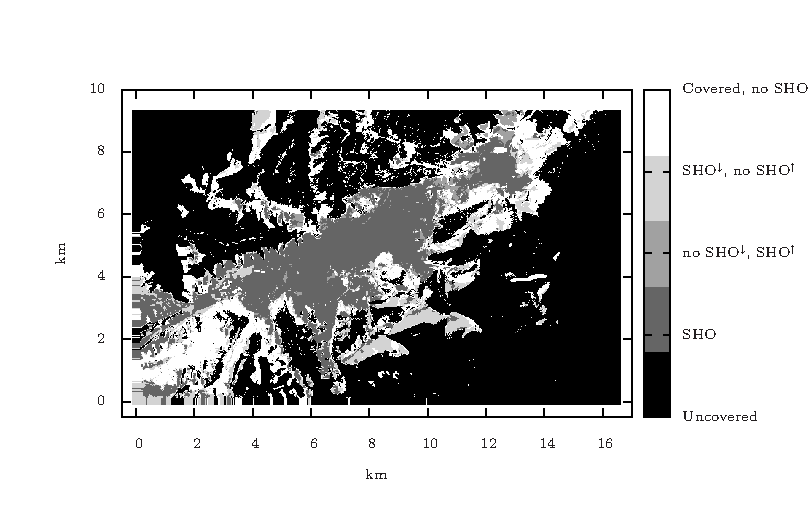
\includegraphics[width=1\textwidth]{07-experimental_evaluation-sho_balancing/img/sho_areas_final}

\caption{Spatial distribution of the SHO areas after the optimization.\label{fig:07-SHO_areas_final}}
\end{figure}


The second most important optimized aspect in the SHO-balancing problem
is the proportion of areas with uplink SHO and no SHO in the downlink
(labeled as `no SHO$^{\downarrow}$, SHO$^{\uparrow}$' in Table~\ref{tab:07-Optimization_result_analysis}).
This particular condition has been improved by almost 17\% in average,
greatly reducing the possibility of interference in neighboring cells
when serving HSPA traffic. The last measured aspect takes into account
areas with downlink SHO and no SHO in the uplink (labeled as `SHO$^{\downarrow}$,
no SHO$^{\uparrow}$' in Table~\ref{tab:07-Optimization_result_analysis}).
This condition, although it hasn't improved, does not expose the mobile
network to malfunctioning, only to reduced throughput within these
specific areas. However, the reduced throughput is relative, since
there are many cells capable of serving HSDPA data access, as the
downlink SHO condition confirms. For this reason, the serving cell
should not only deliver HSDPA, but also take care of the user signaling
and power control, received in the uplink. Clearly, this is only feasible
in areas where uplink coverage is guaranteed.

It is worth mentioning that the simulation results were obtained for
a real radio network with actual configuration data. Moreover, the
hard constraints imposed to the optimization process (the pilot power
limited to the $\pm$2~dB interval) ensure that the resulting configuration
may be immediately applied to a mobile network. This fact can be contrasted
with the spatial distribution of each of the optimized aspects, before
and after applying the optimization results, as it is shown in Figures~\ref{fig:07-SHO_areas_initial}
and~\ref{fig:07-SHO_areas_final}. The lack of any prominent visual
change in Figures~\ref{fig:07-SHO_areas_initial} and~\ref{fig:07-SHO_areas_final}
is a desired consequence of the fine-tuning procedure the network
has been exposed to. Still, the improvements are present precisely
over the areas that are most exposed to malfunctioning due to unbalanced
SHO, e.g., the cell-coverage borders.

\clearpage{}


\section{Summary \label{sec:07-Summary}}

This chapter formally introduced a new optimization problem for 3G
networks: the SHO-balancing problem. A characterization of the consequences
that unbalanced SHO areas have on the quality of HSPA services was
also given. Particularly, tackling the SHO-balancing problem was possible
due to the improved performance delivered by the evaluation framework
PRATO (see Chapter~\ref{chap:04-Framework-design-and-implementation}).

\noindent Using a extension of the radio-network model presented in
Section~\ref{sec:06-Radio_network_model}, Chapter~\ref{chap:06-Experimental-evaluation-the-service-coverage-problem},
the penalty scores of the objective function were set according to
the configuration and layout of a real mobile network, deployed in
Slovenia by Telekom Slovenije, d.d. 

The balancing problem has been tackled by three optimization algorithms,
namely DE, DASA and SA. All three algorithms were able to improve
the given network configuration, being DE the most successful one.
The presented results confirm that a great proportion of the SHO areas,
that were not balanced before the optimization, were corrected, therefore
significantly reducing the possibility of HSPA-service failures. Additionally,
radio coverage was improved, while all other essential network services
were not altered.

One of the key advantages of the presented method is that it targets
the optimization of a deployed network, for which the focus is to
fine-tune the existing configuration instead of creating complete
new solutions. Furthermore, a deployed network has a great number
of hard-constraints that should be taken into account at the optimization
stage. Yet, the presented approach is simple and versatile enough
to be used in practically any working UMTS network. Moreover, the
introduced model is applicable for mobile networks in heterogeneous
environments, because it imposes no restrictions regarding cell layout
or radio-propagation characteristics, which are completely adaptable
through PRATO.

It is important to note that some methods proposed in this chapter
have been particularly designed for problems that emerge during the
planning of 3G radio networks. Despite this, they may be adapted to
other standards, e.g., 2G and 4G, without lose of generality.


\cleardoublepage{}


\chapter{Framework parameter tuning \label{chap:Framework-parameter-tuning}}

% First paragraph has no indentation.

\noindent This chapter \ref{chap:Framework-parameter-tuning} deals
with the automatic tuning of parameters of the mathematical models,
used for radio propagation predictions. Namely, based on field measurements,
the configurable parameters of the mathematical models used by the
framework may be automatically tuned to minize the deviation from
the prediction to the actual state of the network.


\section{Introduction???}

Even after almost 10 years after the launch of the first commercial
UMTS network, service coverage planning remains a key problem that
all mobile operators have to deal with. Its intricacy arises from
the wide range of different combinations of hardware, configuration
parameters and their evaluation-time complexity. 

Although different mathematical models have been proposed for radio
propragation modelling, none of them excels in a network-wide scenario.
A combination of different models and parameters is generally needed
in order to calculate radio-propagation predictions within a bearable
error range. Of course, the number of possible combinations of models
and parameters grows exponentially if we also take into account various
environmental characteristics, such as population density, terrain
relief, land use, and a continously growing number of network cells,
that are indeed compulsory for keeping the error low.

Some of them are more suitable for free space propagation. Others
are better for urban environments, a third groups is even better only
at suburban or rural enviroments. Specifically, when talking about
radio propagation models, threre are manly three clearly distinguishable
groups, namely: statistical models, deterministic models, and combinatorial
models.

Statistical models ... ???

Deterministic ???

Combinatorial ???

Despite an interesting pallete of options of commercial tools, available
for radio propagation modelling, the common thread among all of the
them is the restricted nature of its usage and the lack of adaptation
with cumbersume user interfaces.

In this work, we present a self-adaptive radio propagation tool. The
tool can fine-tune itself before-hand with field measurements in order
to maximize the precision of the radio propagation prediction in the
target area.




\section{Related work???}

In \cite{Ozimek_Open.source.radio.coverage.prediction:2010}, Hrovat
et al. developed a radio planning tool for the GRASS GIS system. Their
work was based on well-known radio propagation models (e.g. Okumura-Hata
and COST 231), and a reverse-engineered one, based on a commercial
tool by Ericsson. The results reported show that the open source radio
planning tool shields comparable results to those of the commercial
tools. Moreover, both tools have similar stddev from field measurements.


\section{Problem description}

Our main objective is improve the quality performance of a given mathematical
model, used for radio-propagation calculations, by fine-tuning its
configurable parameters as per-cell basis. In order to do this, we
will combine field measurements in a feedback loop with an optimization
algorithm over the parameters of the mathematical model.

The idea is to automatically adapt the parameters of the mathematical
model for each of the cells targeted by the optimization. That is,
starting from an a-priori best-known set of parameters, manually calculated
by the radio engineers at Telekom Slovenije, d.d., the algorithm should
optimize the model parameters so that an error measurement of the
radio-propagation prediction to a given set of field measurements
is minimized.

By fine-tuning the model parameters per cell, we achieve region independence
since the field measurements are used as reference. Moreover, we aim
at lowering the error of the model that is tuned for different types
of regions, e.g. urban, suburban and rural. The use of an automated
system, backed by a database, effectively facilitates the daily tasks
of calculating radio-propagation predictions, since the optimized
parameters for a specific cell are directly read from a database.
Therefore, it is feasible for the radio engineer to manage many independent
sets of optimized parameters for numerous cells. Moreover, the user
would decide whether to re-run the parameter optimization, or just
read the already optimized parameters directly from the database.
Additionally, the level of accuracy for the radio-propagation prediction
may be limited, by either setting an optimization-time limit or an
minimum error limit, during which the system fine-tunes the parameters
of the mathematical model.

???

Indeed, based on experimental results showed in \cite{Ozimek_Open.source.radio.coverage.prediction:2010},
we are already confident that well-known models, like Okumura-Hata
and COST 231, provide good results in a feasible amount of time. This
means that with no ``evolved'' mathematical models whatsoever, the
results should be satisfactory for the average case, having the extra
value of the calculation speed gained on GPUs. Moreover, the good
results showed by these well-known models provide a favorable starting
point for the evolution of potential better models.

???


\section{Problem elements}

In this section we introduce all the elements taking part of the self-adaptive
radio propagation tool.


\subsection{Ericsson 9999 model \label{sub:Ericsson-9999-model}}

This radio-propagation model was introduced by Ericsson in 2006, as
an extension of the well-known Hata model {[}ref!Comparison\_2\_11{]},
designed for frequencies up to 2000~MHz. The suitability of this
model comes from the fact that it contains a number of adjustable
parameters, which adapt the model according to a given scenario. Equation
(\ref{eq:ericsson9999}) describes the path loss as evaluated by this
model.

\begin{multline}
pl(d,\beta)=a_{0}+a_{1}\log(d)+a_{2}\log(H_{A})+\\
a_{3}\log(d)\log(H_{A})-3.2\left[\log(11.75\cdot H_{R})\right]^{2}+\\
44.49\log(F)-4.78\left[\log(F)\right]^{2},\label{eq:ericsson9999}
\end{multline}


where $\beta=(a_{0},a_{1},a_{2},a_{3})$ is the vector containing
the tuning parameters of the model, $d$ is the distance (in kilometers)
from the transmitter to the topography point, $H_{A}$ is the effective
antenna height (in meters) of the transmitter, $H_{R}$ is the antenna
height (in meters) of the receiver, and $F$ is the frequency, expressed
in MHz.


\subsection{Differential ant-stigmergy algorithm}

As the optimization algorithm we have chosen the differential ant-stigmergy
algorithm (DASA).

Based on the metaheuristic Ant-Colony Optimization (ACO) \cite{dorigo2006ant_colony_optimization},
the DASA \cite{korosec2010_DASA} provides a framework to successfully
cope with high-dimensional numerical optimization problems. It creates
a fine-grained discrete form of the search space, representing it
as a graph. This graph is then used as the walking paths for the ants,
which iteratively improve the temporary best solution.

The mapping between the balancing problem and DASA is similar to the
one depicted in Equation (\ref{eq:DASA}):

\begin{equation}
X_{a}=\left\{ x_{1},x_{2},\ldots x_{i},\ldots,x_{D}\right\} \label{eq:DASA}
\end{equation}


In this case, each ant, $a$, creates its own solution vector, $X_{a}$,
during the minimization process. At the end of every iteration, and
after all the ants have created solutions, they are evaluated to establish
if any of them is better than the best solution found so far.

There are six parameters that control the way DASA explores the search
space: the number of ants, the discrete base, the pheromone dispersion
factor, the global scale-increasing factor, the global scale-decreasing
factor, and the maximum parameter precision.

For a more in-depth explanation about these parameters and the DASA
algorithm itself, we refer the reader to \cite{korosec2010_DASA}.


\subsection{Field measurements}

The field measurements were taken using a small truck equipped with
the spectrum analyzer Rohde \& Schwarz {[}ref!{]}. The spectrum analyzer
was connected to an external omni antenna mounted on the roof of the
truck, at roughfly 2~meters above the ground, taking measurements
at a rate of ??? per second, with the symbol rate set to ???~Mhz.
To accurately establish the measurement location points, a GPS unit
was used. The measurement locations covered all the streets within
the target area, with over ??? field-measurement points taken at more
than ??? locations. 

To minimize the impact of different driving speed, traffic lights
and other traffic condictions arising during the measurement round,
all field measurements were post-processed so that a single value,
the median, is calculated for each of the measured locations. The
resulting received signal power was used to estimate the path-loss
prediction corresponding to each of the measurements.


\subsection{Optimization objective}

The optimization objective consists of adjusting the parameters of
the Ericsson 9999 model, i.e. $a_{0},a_{1},a_{2},a_{3}$ in Equation
(\ref{eq:ericsson9999}), to best fit a given field-measurement set.
Our data set consists of $N$ data pairs, $(pl_{i},m_{i})$, $i=1,\ldots,N$,
where $N$ is the number of field measurements of the current cell,
$pl(d_{i},\beta)$ represents the path-loss value at measurement point
$i$, as defined in Equation (\ref{eq:ericsson9999}), and $m_{i}$
is the field measurement at the point $i$. By applying the least
squares method {[}ref!{]}, our goal is to minimize the sum, $S^{*}$,
of squared residuals, i.e.

\begin{equation}
S^{*}=\min\sum_{i=1}^{N}r_{i}^{2},\label{eq:cost_function}
\end{equation}


where a residual is defined as the difference between a field measurement
and a path-loss value predicted by the model, i.e.

\begin{equation}
r_{i}=m_{i}-\left[cell\, power-pl(d_{i},\beta)\right].\label{eq:residual}
\end{equation}



\section{Implementation}

As the implementation platform for connecting the different system
components together, we have chosen the open source Geographic Resources
Analysis Support System (GRASS). This Geographic Information System
(GIS) software is used for geospatial data management and analysis,
spatial modeling, and visualization {[}ref!grass{]}. Being an open
system, GRASS provided us with a great deal of essential built-in
functionality, such as functions for displaying results of geographical
maps, importing diffetrent raster and vector formats, database connections
for external attributes, geographical coordinates convertion, etc.
For additional information about the GRASS, we refer the reader to
the numerous guides and tutorials available online.

One of the main reasons for choosing GRASS as our implementation platform
resides in its open nature. This fact helped us not only to achieve
operating-system independence, but most importantly to implement our
system as native GRASS modules. We achieved this by taking advantage
of the very-well documented GRASS Application Programing Interface
(API), which is available for languages such as C and Python. Therefore,
following the modular composition of GRASS itself, we have implemented
a separate GRASS module for each independent component of our system,
namely:
\begin{itemize}
\item the evaluation component, which consists of the modules $r.eric9999$,
$r.sector$ and $db.measurement$; and
\item the optimization component, which consists of a single module called
$dasa$.
\end{itemize}
Figure \ref{fig:system_architecture} depicts the different system
components and the data flow among them.

\begin{figure}
\centering

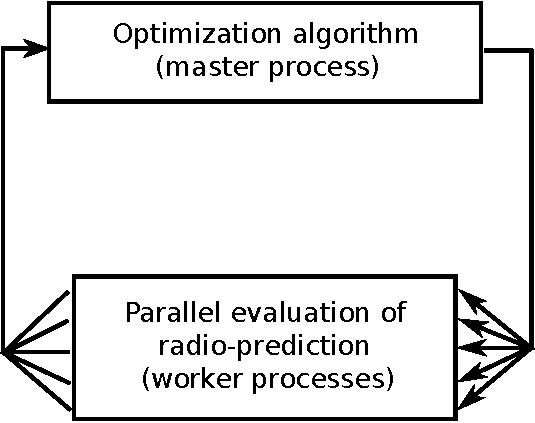
\includegraphics[width=1\columnwidth]{05-framework_parameter_tuning/img/architecture}

\caption{\textit{System architecture and data flow.\label{fig:system_architecture}}}
\end{figure}



\subsection{Evaluation component}

This section describes the different modules that contained in the
evaluation component of the system. Their connections and data flow
is depicted in Figure \ref{fig:evaluation_component}. This particular
component follows a similar internal organization as the radio planning
tool developed by Hrovat et al. \cite{Ozimek_Open.source.radio.coverage.prediction:2010}.

\begin{figure}
\centering


\includegraphics[width=1\columnwidth]{05-framework_parameter_tuning/img/evaluation_component}

\caption{\textit{Evaluation component structure and data flow.\label{fig:evaluation_component}}}
\end{figure}



\subsubsection{Path-loss model}

The module $r.eric9999$ implements the Ericsson 9999 path-loss model,
which was previously introduced in Section \ref{sub:Ericsson-9999-model}.


\subsubsection{Antenna diagram influence}

The module $r.sector$\emph{ }considers the antenna radiation diagram
of the current cell and its influence over the path-loss calculation
of the isotropic source for a specific region. The module uses the
raster map containing the path-loss data for the isotropic source
(i.e. the output of module \emph{$r.eric9999$}), and the radiation
diagram of the antenna, including beam direction, electrical and mechanical
tilt, and antenna gain, as the input data for calculating the actual
path-loss for the currently analyzed cell. The output of this module
is saved in a raster map for further processing. Figures \ref{fig:r_sector_example}
shows an example of applying the $r.sector$ module to output, generated
by the $r.eric9999$ module.

\begin{figure}
\centering


\includegraphics[width=1\textwidth]{05-framework_parameter_tuning/img/pathloss_matrices}

\caption{\textit{Example run of the $r.sector$ module.\label{fig:r_sector_example}}}
\end{figure}



\subsubsection{Received signal strength}

The output of the module $r.sector$ is used as input for calculating
the coverage prediction of the cell being analyzed. Each point within
the raster contains the received signal streght or RSCP {[}ref!{]},
resulting from the combination of the path-loss and the cell transmit
power. The output of module in a raster map for further processing.


\subsubsection{Least squares}

Once the coverage prediction has been calculated and saved, this module
continues the evaluation sequence by comparing each measurement of
the current cell within the area, retrieved from the database with
the module $db.measurement$, with the predicted received signal strength
jus calculated. Consequently, the objective function defined in Equation
(\ref{eq:cost_function}) is applied for each field measurement $i$
to calculate the cost of the current solution $\beta=(a_{0},a_{1},a_{2},a_{3})$.


\subsection{Optimization component}

Because of the metaheuristic nature of the DASA algorithm, it does
not need any problem-specific knowledge to be a good optimization
tool. On the other hand, there are some parameters that influence
the way DASA explores the search space. After some experimental simulations,
we have set the configuration parameters to the following values:
\begin{itemize}
\item $m=10$, the number of ants;
\item $b=10,$ the discrete base;
\item $q=0.2$, the pheromone dispersion factor;
\item $s_{+}=0.01$, the global scale-increasing factor;
\item $s_{-}=0.01$, the global scale-decreasing factor; and 
\item $e=1.0^{-2}$, the maximum parameter precision.
\end{itemize}

\section{Simulations???}


\subsection{Test networks}

All the test networks, $Net_{1}$, $Net_{2}$ and $Net_{3}$ are subsets
of a real UMTS network deployed by Mobitel Telecommunication Services,
Inc. in Slovenia. The path-loss predictions are calculated using the
COST231 model \cite{Cichon_Propagation.prediction.models:1995}, using
a digital evaluation model of 100 $m^{2}$ resolution as input data
and a receiver height of $1.5\, m$ above ground. The requirements
for $SIR$ coverage were provided by experts of the Radio Network
Department at Mobitel Telecommunication Services, Inc.

$Net_{1}$ is deployed over a densely populated urban area. For this
reason, the $SIR$ coverage threshold is a lower, since network capacity
is the dominating factor, whereas coverage is flexible because of
a higher cell density, i.e. more base stations per surface unit. $Net_{2}$
represents a network deployed over a dominant rural area, meaning
that network capacity may be reduced at the cost of better coverage,
since each cell must cover a greater area. The last network, $Net_{3}$,
represents a suburban area with a highly-dense populated, but relatively
small, downtown center, where a compromise between network capacity
and coverage has to be achieved.

Based on the data available, we have produced network configurations
based on the attenuation-based approach. These configurations represent
what could be an initial network setup by common planning standards
\cite{Holma_WCDMA.for.UMTS:2005}. Moreover, such configurations are
also very straightforward to calculate by a network planner. Table
\ref{tab:network-statistics-1} shows some statistics of the test
networks used. The parameter values used during experimentation are
shown in Table \ref{tab:network-parameters-1}.

\begin{table}
\caption{\textit{Network statistics.\label{tab:network-statistics-1}}}


\centering

\begin{tabular}{ccc}
\toprule 
 & Cells $[m]$ & Area $[km^{2}]$\tabularnewline\addlinespace
\midrule
$Net_{1}$ & 77 & 100\tabularnewline
$Net_{2}$ & 23 & 306.25\tabularnewline
$Net_{3}$ & 129 & 405\tabularnewline
\bottomrule
\end{tabular}
\end{table}


\begin{table}
\caption{\textit{Network parameters.\label{tab:network-parameters-1}}}


\centering

\begin{tabular}{clll}
\hline 
Parameter & $Net_{1}$ & $Net_{2}$ & $Net_{3}$\tabularnewline
\hline 
$p_{c}^{T}$ & 15.00 W & 19.95 W & 15.00 W\tabularnewline
$\tau_{0}$ & 1.55$\cdot10^{-14}$ W & 1.55$\cdot10^{-14}$ W & 1.55$\cdot10^{-14}$ W\tabularnewline
$\gamma_{c}$ & 0.01 & 0.02 & 0.015\tabularnewline
\hline 
\end{tabular}
\end{table}



\subsection{Algorithm parameter settings \label{sub:Algorithm-parameter-settings-1}}

After short experimentation, we determined the parameter settings
for the optimization algorithm. There was no fine tuning of parameters
for each problem instance. Nevertheless, we gained valuable information
regarding the agent's behavior that we used to set the following parameter
values:
\begin{itemize}
\item $increase\, rate$ was set to 0.2 dB;
\item $decrease\, rate$ was set to -0.1 dB;
\item $number\, of\, agents$ was set to 16; and
\item 10,000 $changes\, per\, agent$ were allowed.
\end{itemize}

\subsection{Experimental environment}

All experiments were done on a 4-core, hyper-threading, Intel i7 2.67
GHz desktop computer with 6 GB of RAM running a 64-bit Linux operating
system. The GPU hardware was ATI HD5570, with 1 GB DDR3 RAM. The implementation
language used was C, with OpenCL and OpenMPI extensions.


\subsection{Optimization results}

The results achieved by our optimization approach improved the objective
significantly, as it is shown in Table \ref{tab:optimization-results-2}.
Results show that we reduced pilot power usage in all networks and
kept the service area under full coverage. Moreover, we may see the
solution for $Net_{1}$ improved the attenuation-based setting by
more than 300\%. For $Net_{2}$, the improvement observed is around
232\%, with an improvement of more than 170\% for $Net_{3}$. These
means that network capacity has been significantly increased in all
three problem instances. Therefore, a greater number of users should
be able to access services provided by the mobile network, since coverage
is assured. Moreover, an increased speed in data services should be
observed \cite{Holma_WCDMA.for.UMTS:2005}.

\begin{table}
\caption{\textit{Optimization results.\label{tab:optimization-results-2}}}


\centering

\begin{tabular}{cccccc}
\toprule 
 & \multicolumn{2}{c}{Attenuation-based} &  & \multicolumn{2}{c}{Parallel agents}\tabularnewline\addlinespace
\cmidrule{2-3} \cmidrule{5-6} 
 & Total power {[}W{]} & Average cell power {[}W{]} &  & Total power {[}W{]} & Average cell power {[}W{]}\tabularnewline\addlinespace
\cmidrule{1-3} \cmidrule{5-6} 
$Net_{1}$ & 419.292 & 5.445 &  & 137.064 & 1.780\tabularnewline
$Net_{2}$ & 78.297 & 3.404 &  & 33.344 & 1.450\tabularnewline
$Net_{3}$ & 1,014.113 & 7.861 &  & 582.954 & 4.519\tabularnewline
\bottomrule
\end{tabular}
\end{table}


After collecting data from ten independent runs, we generated convergence
graphs, shown in Figures ???. The graphs contain feasible solutions
only, i.e. solutions that meet the full-coverage constraint. Unfeasible
solutions were marked with a value of inferior quality than the worst
solution found by the algorithm in all ten runs. In case of $Net_{1}$,
the value was set to 428, for $Net_{2}$ the value was set to 129
and for $Net_{3}$ the value was set to 1,435. 

The analysis of convergence graphs of $Net_{1}$ and $Net_{2}$ shows
that the algorithm quickly converges at the beginning, followed by
a steady improvement of intermediate solutions. In $Net_{1}$ we notice
additional improvement of the solutions found even at towards the
end. This fact suggests that longer runs would potentially find even
better solutions in this case. For the instance $Net_{3}$, we observe
a slower initial convergence, with steady improvement of intermediate
solutions and no significant solution enhancement towards the end.
This fact, together with the aforementioned results, suggest that
this problem instance presents a more difficult optimization case
than $Net_{1}$ and $Net_{2}$. Further investigation would be needed
to determine the source of this behavior. Nevertheless, the improvement
observed is, in average, around 100\%.


\section{Conclusion???}

In this paper, we have addressed the problem of providing full coverage
to a service area of a UMTS network by using a minimum amount of pilot
power. We have put emphasis on the confluence of a real-world problem,
with live data from a deployed mobile network, with state-of-the-art
parallel GPU hardware and implementations that, to the best of our
knowledge, has never been dealt-with before.

We have presented a parallel-agent approach, which is aimed at giving
good solutions to big problem instances in an acceptable amount of
time. The experimental results show that our approach is able to find
competitive solutions, when compared to other common radio-planning
methods \cite{Holma_WCDMA.for.UMTS:2005}. The presented results also
demonstrate that our algorithm is able to find high quality solutions
even for large networks, that contain many cells over a large service
area. This fact indicates that our approach could be successfully
applied to bigger problem instances.

GPU architectures not only allow implementation of parallel heuristics
in a natural way, they also substantially improve the performance
of the optimization process. We reported and validated the great performance
gain by experimentation on problem instances of different sizes.

After successfully implementing the objective-function evaluation
on GPU, we realized that the efficiency of this approach was limited
by the CPU-to-GPU data transfers. Nevertheless, even with such implementation,
we have already obtained substantial speed-up.

To deal with the CPU-to-GPU data transfer issue, we implemented a
fully-enabled GPU optimization system that achieved impressive speed-up.
Still, we had to consider different data representation schemes for
the problem elements, so to avoid memory limitations on the GPU device.
Comparison of our experimental results with other algorithms dealing
with the same and similar problems would be useful. However, this
task is not straightforward, since the results of several works (e.g.
\cite{Gerdenitsch_PhD:2004,Turke_Advanced.site.configuration.techniques:2005})
depend on black-box evaluations, making experimental association very
difficult, if possible at all. 

All in all, we consider that the present work provides a robust foundation
for future work on grid-based metaheuristics with expensive objective-function
evaluation.

In future work, we will consider further analysis of our parallel-agent
approach, including experimentation with different parameters, in
order to gain better understanding of the dynamics leading the metaheuristic
during the search process. Multi-GPU environments present an interesting
possibility, where evaluator(s) and worker agents are run on separate
GPU devices.


\cleardoublepage{}


\chapter{Performance assessment within real network-planning scenarios}

% First paragraph has no indentation.

\noindent About the framework compiting with industrial tools in terms
of quality and speed performance.


\cleardoublepage{}


\chapter{Conclusion and further work \label{chap:Conclusion}}

Fast and accurate performance evaluation is of essential importance
for the planning and optimization of mobile radio networks. In this
thesis, several high-performance and novel methods for the analysis
and optimization of radio networks were developed and discussed. Some
of them even outperform state-of-the-art methods, to which they were
compared, in terms of result accuracy and instance-size complexity.

The snapshot analysis is best suited for the detailed performance
evaluation of radio networks. The performance of a snapshot method
is mainly influenced by two factors. First, the performance of the
method for modeling a single snapshot and, second, the quality level
of the estimate applied for obtaining the interest figures from the
individual snapshot results. Both topics were comprehensively addressed
in this thesis.

While providing detailed and accurate results for various applications
in network planning, the snapshot analysis is too time-consuming to
be applied in radio-network optimization, where typically a large
number of different configurations need to be compared in a shorter
time-frame. To this end, a parallel framework for radio-network planning
was presented in this thesis. The framework is very flexible in terms
of air-interface modeling, e.g., different QoS schemes, and is of
significantly higher computational-time performance compared with
any currently available solution known to the author. Moreover, it
incorporates multi-GPU support and the corresponding parallel-programming
techniques that are required to exploit the computational power of
such hardware. The performance gain results mainly due to the combination
of a novel parallel-programming approach and some state-of-the-art
methods. The achieved performance improvement excels in radio-network
optimization environments. Further research in this field will include
abstracting the introduced MWD principle into a multi-purpose parallel
framework such as Charm++~\cite{Kale-The_Charm_Approach:2013}, which
provides a functionality for overlapping execution and communication,
as well as fault tolerance.

When applying automatic network optimization, a fast and accurate
performance analysis is of crucial importance. However, an overview
of the related literature shown that this fact seems to have been
only partially taken into consideration in the design of several optimization
methods for radio networks. A common approach is to apply a detailed
and too time-consuming method for evaluating different candidate solutions,
resulting in an unacceptable computational-time complexity for medium
to large-sized problem instances. The opposite approach, which is
even less satisfactory, is to build fast but inaccurate models, the
results of which do not sufficiently correlate with reality. To this
end, the quality and speed performance of the presented framework
was empirically verified with an industrial software tool for radio-network
planning. The results clearly show a very good agreement in terms
of accuracy of the radio-propagation predictions, compared to those
obtained with the commercial tool. Additionally, the results demonstrated
the performance advantage of the framework compared to the computational
time of the enterprise software. It is important to note that these
results also apply for an application in everyday network planning.
However, to ultimate validate the complete array of radio-planning
activities the framework can handle requires some further research,
which has already started.

Increasing the performance of the simulations involved during the
objective-function evaluation is only the first step towards a practical
running-time reduction for radio-network optimization. In this sense,
the performance of the novel agent-based algorithm presented in this
thesis was tested while solving the service-coverage problem in radio
networks. The results show significant gains with respect to the size
of problem instances, as well as regarding its speed performance and
solution quality, even outperforming a state-of-the-art method, to
which it was compared. Further research will include experimentation
with different parameters and optimization problems, in order to gain
better understanding of the dynamics that guide the algorithm through
the search space of the problem.

The new optimization problem for 3G radio networks indentified in
this thesis deals with SHO balancing of downlink and uplink areas.
The problem was tacled by three different metaheuristic algorithms,
the solutions of which show a substantial improvement of downlink
and uplink balance. A challenge for future work is to evaluate this
optimization problem in a dynamic context. This requires using a full-stack
simulation tool that includes dynamic effects, such as fast power
control.

The clutter-loss optimization method developed in this thesis makes
use of the tools discussed above, providing a faster, more accurate
and simpler method that replaces a manual approach. It applies a metaheuristic
algorithm which has been tailored for the special requirements of
the automatic clutter-loss optimization. The presented results make
the benefits of an automated-optimization approach evident. Furthermore,
in the context of other radio-coverage planning activities carried
out at the Radio Network department of Telekom Slovenije, d.d., supplementary
testing of the framework as a coverage-planning tool is currently
being conducted.

PRATO, the radio-planning framework presented is this thesis, is free
and open-source software. For this reason, it can be readily modified
and extended to support, for example, other propagation models and
post-processing algorithms. This characteristic provides it with a
clear advantage when compared to commercial and closed-source tools.
The source code is available for download from the author's home page,
http://csd.ijs.si/benedicic/.

The constantly improving performance of computer hardware might allow
an even more detailed analysis of networks in the near future. In
this sense, a major challenge, that will require further research,
is to extend the presented models and algorithms, e.g., by incorporating
user mobility and traffic dynamics. This is especially important due
to different existing and emerging mobile technologies. Indeed, the
co-existence of multiple technologies will motivate an increasing
interest about the combined analysis and optimization of different
technologies and their mutual dependency.


\section{Scientific contributions}

The work in this thesis has led to the following original contributions
to science:
\begin{enumerate}
\item Design and development of an unified framework for radio-network planning
and optimization, incorporating the second and third items, as well
as experimentation on real-world radio networks. The experimentation
includes a comparison with a commercial tool that is currently being
used for real radio-network planning. Moreover, the parallel implementation
of the framework exploits the computing resources of computer clusters
and GPUs.
\item Proposal of a new approach for parallel programming that combines
a classic master-worker method with an external database. The proposed
approach improves the scalability of the classic master-worker paradigm
by preventing the master process to become the bottleneck of a parallel
system.
\item Quality improvement of radio-propagation predictions by applying metaheuristic-optimization
techniques that improve the quality of results. This technique enables
the adaptation of radio-propagation models to the local environment
over which a radio network is deployed, as well as the automatic optimization
of signal losses due to clutter.
\item A new algorithm, based on autonomous agents, to tackle the service-coverage
problem in radio networks. The algorithm deals with problem instances
that are out-of-reach of other compared state-of-the-art techniques
used as reference. It also reaches good quality of solutions if compared
to classic network-planning techniques. The proposed approach is especially
suitable for optimizing large radio networks.
\item Identification and formalization of a new optimization problem in
3G radio networks that deals with SHO alignment of downlink and uplink
areas. By solving this problem, network malfunctioning is avoided
in areas where there is SHO capability in the uplink, but none in
the downlink. So far, this problem has not been formalized nor tackled
by means of automatic optimization.\end{enumerate}



\cleardoublepage{}

\bibliographystyle{plain}
\bibliography{01-introduction/01-introduction,02-background_and_motivation/02-background_and_motivation,04-framework_design_and_implementation/04-framework_design_and_implementation,06-experimental_evaluation-service_coverage/06-service_coverage_problem,07-experimental_evaluation-sho_balancing/07-soft_handover_alignment,05-framework_parameter_tuning/05-framework_parameter_tuning}


\cleardoublepage{}


\chapter{Acknowledgments}

% First paragraph has no indentation.

\noindent The authors would like to especially thank the radio engineers
at Telekom Slovenije, d.d., for cooperating and sharing their professional
expertise throughout the creation of this work. This project was co-financed
by the European Union, through the European Social Fund.

The contents presented in Chapter \ref{chap:Framework-design-and-implementation}
are the results of joint research work, conducted with the Nagasaki
Advanced Computer Center (NACC) of the Nagasaki University. In this
context, T. Hamada, head of NACC, acknowledges support from the Japan
Society for the Promotion of Science (JSPS) through its Funding Program
for World-leading Innovative R\&D on Science and Technology (First
Program).

\end{document}
